\chapter{Optimierung einzelner Parameter}
\label{chap:parameteruntersuchung}

Grundlegend kann die Parameteruntersuchung wie eine Art Entscheidungsbaum aufgefasst werden. Dabei führt jede Entscheidung im Baum zu einer neuen Untersuchung und zu neuen Erkenntnissen. Im Verlaufe dieser Untersuchung werden somit Konzepte, Flugzustände, Komponenten und Konfigurationen ausgewählt und intensiver betrachtet. Den Beginn zeichnet die grundlegende Frage aus, welches Fluggerätekonzept, i.e. Flächenflugzeug oder Multicopter, sich für einen effizienten Aufstieg in die untere Stratosphäre als optimaler erweist. \\
In der folgenden Parameteruntersuchung sei nochmal auf den Aufbau der Leistungsberechnung verwiesen, der dem eines realen Systems in umgekehrter Weise gegenübersteht (Kap. \ref{sec:flugleistungsberechnung}).

\section{Multicopter im Vergleich zu einem Flächenflugzeug}
\label{sec:multicopter_vs_flaechenflugzeug}
Jedes Luftfahrzeugkonzept entzieht sich einem direkten Vergleich mit einem Luftfahrzeug einer anderen Art. So weist jedes Fluggerät in seiner Gattung spezifische Vorteile auf wie der Start auf der Stelle und das Hovern in der Luft für Multicopter oder der Gleitflug für Flächenflugzeuge. Die optimale Auslegung beider führt zu unterschiedlichen Designs was die Propeller, die Motorleistung und -gewicht, Größe, Gesamtgewicht etc. betrifft. Aus diesem Grund müssen Kriterien für eine Vergleichbarkeit vorgeschrieben werden. Hierfür wird das Design des Multicopters auf das aus \cite{Anderson.2018} festgelegt, welches genauer in Kapitel \ref{sec:komponenten} beschrieben ist. Da die Flugleistungen von \cite{Anderson.2018} bekannt sind und der Quadrocopter durchaus schon im Rahmen der Anforderungen für diese Mission als optimiert betrachtet werden kann, bedarf es lediglich einer Untersuchung des Flächenflugzeuges. Dazu wird das Flächenflugzeug auf Parameter fixiert, mit denen es bereits sehr hoch aufsteigen kann. Zur Untersuchung und Vergleichbarkeit werden beide Gesamtmassen gleichgesetzt \ensuremath{m_{ges,Quadrocopter} = m_{ges,Flächenflugzeug}}. Dabei setzt sich die Masse der Flächenflugzeugbatterie   
\begin{equation}
	m_{Bat,Fl} = m_{Bat,Quad} + (m_{Mot,Quad}\cdot n_{Prop,Quad} - m_{Mot,Fl}\cdot n_{Prop,Fl}) - (1-f_P)\cdot m_{Quad}  
\end{equation}
in Bezug auf bereits gewählte Massen und auf den Quadrocopter zusammen. Der Faktor \ensuremath{f_P} kann als Penalty-Faktor verstanden werden. Dieser verringert zusätzlich die Batteriemasse, wenn das Strukturgewicht des Flächenflugzeugs das des Quadrocopters überschreitet
\begin{equation}
	f_P = \frac{m_{Flugzeug}}{m_{Quad}} \eqend{.}
	\label{eq:penalty}
\end{equation} 
Für erste Untersuchungen wird der Penalty-Faktor auf 1 gesetzt. Dies entspricht einer optimistischen Einschätzung. Im Anschluss werden die Parameter in näherer Umgebung der ersten festgesetzten Werte variiert. Dadurch kann der Einfluss auf das Leistungsverhalten und die Richtung der Optimierung bestimmt werden. Diese erste, einfache Untersuchung ist nur eine sehr oberflächliche, weil jeder Parameter nur einzeln untersucht wird. Jegliche Kombinationen von Einflüssen wie der Einfluss des Masse auf die Steiggeschwindigkeit oder vergleichbare Beziehungen werden vernachlässigt. Im Hinblick auf diese erste, kleine Optimierung ist der Kostenfaktor die maximal erreichbare Höhe beider Fluggeräte. Je nachdem welches der beiden Fluggeräte effektiver und effizienter eine maximale Flughöhe erreicht, wird es weiter untersucht und anschließend optimiert.  

In der Tab. \ref{tab:referenzkonfiguration} sind wichtige Parameter der Ausgangskonstellation für das Flächenflugzeuges aufgelistet. Die Werte wurden in ersten Untersuchungen festgelegt. 
\todo[inline]{wie genau wurden die ersten Werte bestimmt?}
\begin{center}
	\captionof{table}{wichtige Parameter der Flächenflugzeug-Referenzkonfiguration}
	\begin{tabular}{l l l} \hline
		Parameter & Variablenname & verwendete Größe \\ \hline
		Leermasse des Flächenflugzeug \ensuremath{m_{Flugzeug}}& \texttt{m\_Flugzeug} & \SI{0,354}{kg} \\ 
		Batteriemasse \ensuremath{m_{Bat}} & \texttt{m\_Bat} & \SI{0,56}{kg} \\
		Motormasse \ensuremath{m_{Mot}}& \texttt{m\_Mot} & \SI{106}{g} \\
		Geschwindigkeitskonstante \ensuremath{K_V} & \texttt{K\_V} & \SI{1390}{RPM/V} \\
		maximaler Dauerstrom \ensuremath{I_{max}} & \texttt{I\_max} & \SI{35}{A} \\
		Propeller & \texttt{prop\_name} & 9x7 \\
		Anzahl Propeller \ensuremath{n_{Prop}} & \texttt{n\_prop} & \SI{1}{} \\
		Auslegungsgleitzahl \ensuremath{E^{\star}} & \texttt{E\_stern} & \SI{4}{} \\
		Auslegungsgeschwindigkeit \ensuremath{V^{\star}} & \texttt{V\_stern} & \SI{100}{km/h} \\
		Gleitzahl \ensuremath{E} & \texttt{E} & \SI{4}{} \\ 
		Anzahl der Batteriezellen \ensuremath{N_{Bat,cell}} & \texttt{N\_bat\_cell} & 6 \\	
		Penalty-Faktor \ensuremath{f_P}	& \texttt{f\_P}	& 1 \\ \hline
	\end{tabular}	
	\label{tab:referenzkonfiguration}
\end{center}
Diese Konfiguration ist die Grundlage aller Untersuchungen, die das Flächenflugzeug betreffen.



\begin{figure}[H]
%\centering
	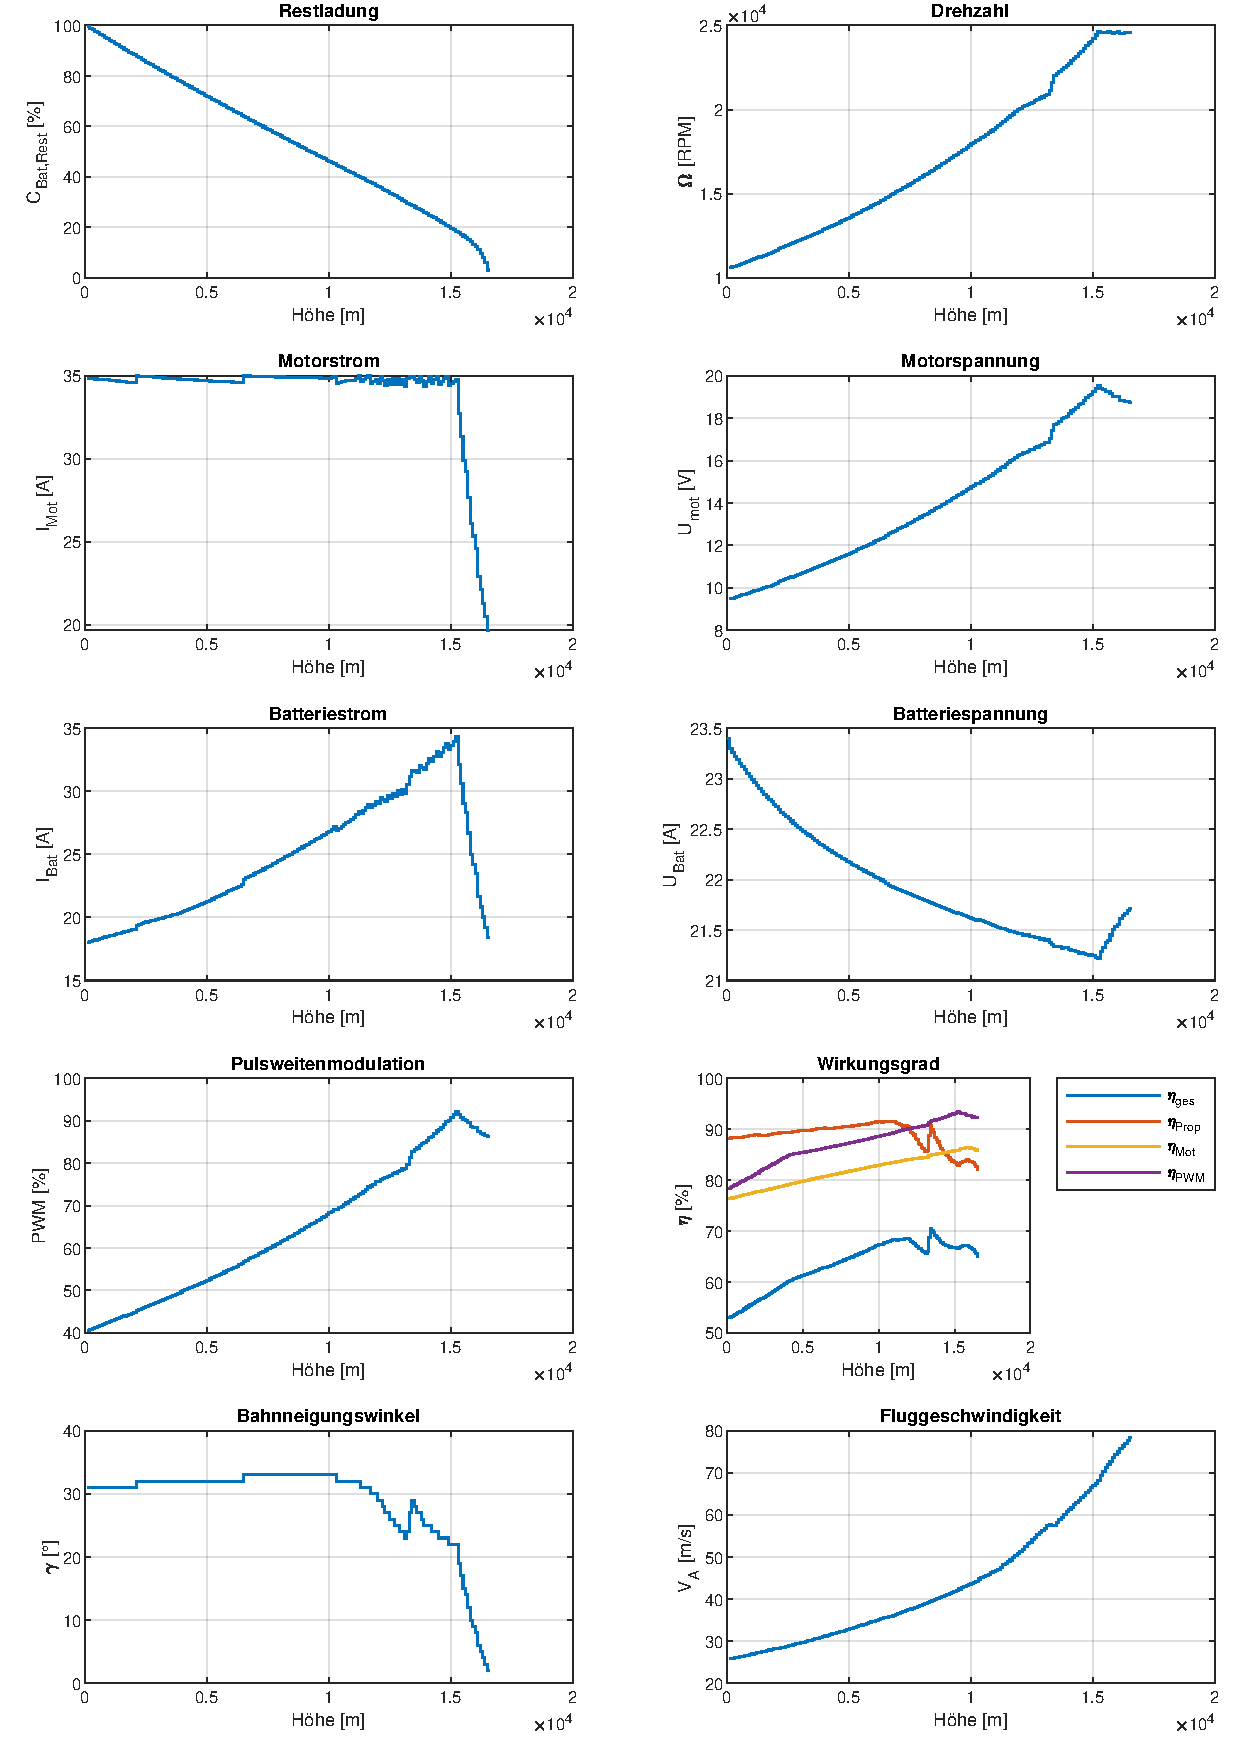
\includegraphics[scale=0.7]{Diagramme/Ausgangskonstellation.pdf}
	\caption{Verlauf der Leistungsparameter über der Höhe für die Flächenflugzeug-Referenzkonfiguration (Tab. \ref{tab:referenzkonfiguration})}
	\label{abb:referenzkonfiguration}
\end{figure}
Die in Tab. \ref{tab:referenzkonfiguration} beschriebene Referenzkonfiguration erreicht bereits eine Flughöhe von \SI{16500}{m}. Der limitierende Parameter für den Aufstieg in noch größere Höhen ist in diesem Fall nicht die Motorleistung, sondern die maximale Propellerdrehzahl (Vgl. Abb. \ref{abb:referenzkonfiguration}). Eine Erhöhung der Drehzahl ist in diesem Fall durch zwei Einflussfaktoren nicht möglich. Zum einen ist die maximale Propellerdrehzahl auf \SI{25000}{RPM} durch das Ende des Kennfeldes begrenzt. Dies ist mit hoher Wahrscheinlichkeit auf die Festigkeit des Propellers zurückzuführen. Bis zu dieser Drehzahl ist ein uneingeschränkter Betrieb des Propellers möglich, ohne das ein strukturelles Versagen des Propellers zu befürchten ist. Ab einer höheren Drehzahl kann ein sicherer Betrieb nicht mehr gewährleistet werden. Der zweite Einflussfaktor ist die Blattspitzengeschwindigkeit \ensuremath{Ma_{tip}}. Diese erreicht ab \SI{15000}{m} Höhe \ensuremath{Ma_{tip} = 1}. Damit kommt es zu Machzahleffekten und einer relativen Überschallanströmung an der Propellerspitze. Die dadurch verursachten zusätzlichen Verluste (z.B. Stoßverluste), Stömungsablösungen, Verminderungen in der Schuberzeugung usw. können nicht in dem einfachen Luftmodell berücksichtigt werden, das dem in Kap. \ref{chap:Programmbeschreibung} erläuterten Programm zur Flugleistungsberechnung zugrunde gelegt wurde. An dieser Stelle können transsonische Effekte, die bereits bei einer relativen Anströmung an der Propellerspitze von \ensuremath{Ma < 1} auftreten können, nicht ausgeschlossen werden. Es gibt zwei Möglichkeiten, die Limitierung der Flughöhe durch die Propellerdrehzahl zu vermeiden. Zum einen kann ein Propeller mit größerer Steigung gewählt werden. Mit der größeren Steigung ist es möglich denselben Schub bei verringerter Drehzahl zu erzeugen. Die andere Möglichkeit umfasst eine Vergrößerung des Propellerdurchmessers.
\todo[inline]{Quelle van der Wall}
 Mit diesem steigt die Effizienz  und führt zu demselben Effekt wie oben beschrieben.  \\
Die Limitierung der Flughöhe durch die maximale Propellerdrehzahl stellt eine Dienstgipfelhöhe dar. Diese limitiert den Steigflug bereits zu Beginn des Starts auf \SI{16500}{m}. Eine Erhöhung der Motorleistung, der Batteriezellenanzahl oder beispielsweise der Kapazität würde keine weiteren Verbesserungen der Flugleistungen erbringen, da die Begrenzung durch die Propellerdrehzahl für jeden Flug dieselbe ist. Generell ist eine Erhöhung des Leistungsüberschuss (\ensuremath{=} Erhöhung der Leistung) damit nicht zielführend. Ein Steigflug ohne Dienstgipfelhöhe zeichnet sich durch die Limitierung der Flughöhe durch die Restladung aus. Hierbei sinkt diese linear ab bis \SI{0}{\%} Restladung erreicht sind. \\
Das Erreichen der Dienstgipfelhöhe zeichnet sich durch eine Verschlechterung Flugleistungen aus. Die Restkapazität nimmt mit der Höhe linear ab. Ab der Höhe von \SI{15000}{m} wird die maximale Propellerdrehzahl erreicht, sodass sich die Abnahme der Restkapazität erhöht. \\
Der Steiflug bis \SI{15000}{m} ist durch den Betrieb bei maximalem Dauerstrom (\ensuremath{I_{max} = \SI{35}{A}}) gekennzeichnet. Dadurch stellt sich ein optimaler Bahnneigungswinkel von \SI{31}{^\circ} bis \SI{33}{^\circ} ein. Dieser Winkel kann bis zu einer Höhe von \SI{10000}{m} gehalten werden, bevor er zunächst langsam absinkt und ab \SI{15000}{m} steil gegen \SI{0}{^\circ} strebt. Die Fluggeschwindigkeit steigt mit dem Steigwinkel leicht progressiv mit dem Produkt aus \ensuremath{\sqrt{\rho^\star/\rho}} an (Vgl. Gleichung \ref{eq:geschw_flaechenflugzeug}). \\
Zu Beginn des Steigfluges wären größere Steigwinkel effizienter, allerdings werden diese durch den maximalen Motorstrom \ensuremath{I_{max}} begrenzt. Ohne diesen würde der Bahnneigungswinkel beinahe linear absinken. Daraus kann geschlossen werden, dass ein Flug mit maximalem Motorstrom im unteren Höhenbereich am effizientesten ist. Der sägezahnartige Verlauf des Motorstroms hängt mit der gewählten Diskretisierung und dadurch rückwirkend mit der Genauigkeit zusammen. Eine genauere Untersuchung der in den Diagrammen dargestellten Punkte und deren Umgebung würde zu einem glatten Verlauf des Motorstroms bei \ensuremath{I_{max}} führen. Ebenso würden sich die Verläufe aller anderen Leistungsparameter über der Höhe glätten. Gleichzeitig zum konstanten Motorstrom wächst die Motorspannung linear an, bis diese ab \SI{9800}{m} das Niveau der Batteriespannung erreicht. \\
Auch die Propellerdrehzahl weist eine leicht progressive Zunahme auf. Mit der Höhe sinkt die Dichte entsprechend nach Gleichung \ref{eq:rho_0_11} und \ref{eq:dichte_strato}. Zur Erzeugung des gleichen Schubs muss mit der abnehmenden Dichte die Drehzahl steigen, um den Massenstrom durch die Propellerebene und letztendlich den Schub konstant zu halten (Vgl. Gleichung \ref{eq:propellerschub}). Bei konstantem Motorstrom und steigender Propellerdrehzahl nimmt entsprechend auch die Motorspannung zu (Vgl. Gleichung \ref{eq:motorspannung}). \\
Der Verlauf des Batteriestroms steht in direktem Zusammenhang mit dem Motorstrom und der Motorspannung. Dies wird aus Gleichung \ref{eq:batteriestrom} ersichtlich. Bei einem konstantem Motorstrom ist  \ensuremath{I_{Bat}} nur von \ensuremath{U_{Mot}} abhängig. Daher der gleiche Verlauf wie bei \ensuremath{U_{Mot}}. Ab dem Erreichen der maximalen Propellerdrehzahl nimmt \ensuremath{U_{Mot}} wieder leicht ab und \ensuremath{I_{Bat}} hängt nur noch von \ensuremath{I_{Mot}} ab. Der Verlauf der Drehzahl ist ausschlaggebend für die Motorspannung. Die Batteriespannung bricht durch die Belastung von anfänglichen \SI{23,4}{V} auf \SI{21,2}{V} ein. 
Die PWM steigt mit dem Verlauf der Motorspannung sowie der Batteriespannung an. Ab \SI{15000}{m} erreicht sie ihr Maximum bei \SI{91,5}{\%}. Dies verdeutlicht noch einmal, dass für die Referenzkonfiguration die Motorleistung nicht die den die Höhe limitierenden Leistungsparameter darstellt. \\
Ist die maximale Propellerdrehzahl ab \SI{15000}{m} erreicht, fällt der Motorstrom rapide mit der konstanten Drehzahl ab. Da die Drehzahl konstant bleibt bis zum TOC, nimmt das Propellerdrehmoment und damit auch der Motorstrom mit zunehmender Höhe und abnehmender Dichte ab (Vgl. \ref{eq:motorstrom}). Mit sinkendem Motorstrom sinkt auch die Motorspannung  (Vgl. Gleichung \ref{eq:motorspannung}) und schließlich die PWM (Vgl. Gleichung \ref{eq:pwm}). Dieser Effekt wird noch durch den Anstieg der Batteriespannung auf \SI{21.7}{V} verstärkt. Der sinkende Propellerschub bei konstanter Drehzahl hat außerdem ein Sinken des Bahnneigungswinkels \ensuremath{\gamma} zur Folge. Der sinkende Schub reicht für größere Bahnneigungswinkel nicht mehr aus. Mit diesem Streben der Restladung und des Bahnneigungswinkel gegen null ist die Dienstgipfelhöhe erreicht, ab der kein weiter Steigflug mehr möglich ist. Jedoch würde auch ohne diese Begrenzung der TOC nur ein paar hundert Meter höher liegen, wenn die Restladungskurve linear extrapoliert würde. \\
Der kurze Sprung im Bahnneigungswinkel, der sich durch alle anderen Diagramme fortpflanzt, kann auf eine Inkonsistenz im Kennfeld oder Berechnungsfehler zurückverfolgt werden.\\
Der Gesamtwirkungsgrad gliedert sich wie in Kap. \ref{subsec:eta_ges} dargelegt in den Propeller-, den Motor- und den Motorreglerwirkungsgrad. Daher folgt er zeitgleich den anderen Wirkungsgraden. Der Propellerwirkungsgrad steigt mit der Höhe an. Ausschlaggebend hierfür ist die steigende Geschwindigkeit und die Drehzahl (Vgl. Gleichung \ref{eq:eta_prop}). Während der Bahnneigungswinkel ab \SI{10000}{m} abfällt, steigt die Bahngeschwindigkeit und der Propellerwirkungsgrad. Über Gleichung \ref{eq:geschw_flaechenflugzeug} nimmt mit steigendem Bahnneigungswinkel die Fluggeschwindigkeit ab. Da dieser jedoch nun absinkt, nimmt damit im Umkehrschluss die Fluggeschwindigkeit zu. \\
Da die Motorspannung bereits ihr Maximum erreicht hat, kann die Propellerdrehzahl nur noch leicht mit der abnehmenden Dichte und somit geringer werdenden Widerstandskräften ansteigen (Vgl. Gleichung \ref{eq:motorspannung}). Dabei nimmt auch das Propellerdrehmoment ab (Ergebnis aus Gleichung \ref{eq:motorstrom}). Bei einer gleichermaßen steigenden Fluggeschwindigkeit, steigt die Strahlleistung des Propellers (Vgl. Gleichung \ref{eq:strahlleistung}). Als Konsequenz steigt der Propellerwirkungsgrad.
Dies gilt auch für den Motorwirkungsgrad. Dieser steigt mit einer anwachsenden Propellerdrehzahl und -drehmoment (Vgl. Gleichung \ref{eq:eta_mot}). Außerdem nehmen die durch den Innenwiderstand und den Leerlaufstrom verursachten Verluste anteilig am Motorstrom und der -spannung ab (Vgl. Gleichung \ref{eq:motorstrom} und \ref{eq:motorspannung}), die mit zunehmender Höhe auch zunehmen. Der Grund hierfür liegt in der Annahme, dass diese beiden Motorkenngrößen für jeden Motorzustand als konstant angesehen werden. Der Wirkungsgrad des ESC steigt simultan mit der Höhe und der PWM. Mit steigender PWM nehmen auch die Verluste innerhalb des Motorreglers ab (Vgl. Gleichung \ref{eq:eta_pwm}). Deutlich zu erkennen ist eine leichte Abnahme aller Wirkungsgrade ab \SI{15000}{m}. Der Propellerwirkungsgrad nimmt dabei deutlich schneller ab. Die Begründung kann in dem abnehmenden Schub und die mit konstanter Drehzahl abnehmende induzierte Geschwindigkeit gefunden werden. Dies ist ein Indiz für den Beginn eines ineffizienteren Flugzustandes.



\section{Einflussfaktoren auf das Flächenflugzeug}
Die zu variierenden Parameter des Flächenflugzeugs sind diejenigen Leistungsparameter, die das Fluggerät qualifizieren. Das sind die Motor-Propeller-Kombination, die Propelleranzahl, die Gleitzahl, die Auslegungsgeschwindigkeit und der Penalty-Faktor.

\subsection{Motor-Propeller Kombination}
\label{subsec:mot_prop_kombi}
Die Motor-Propeller-Kombination beeinflusst entscheidend das Leistungsverhalten von elektrisch, propellergetriebenen Fluggeräten. Mit dem in Tab. \ref{tab:referenzkonfiguration} aufgeführten Motor mit einem Gewicht von \SI{106}{g} und einem \ensuremath{K_V}-Wert von \SI{1390}{RPM/V} sind bereits sehr hohe Flughöhen erreichbar. Bei Verwendung des gleichen Propellers, einem 9x7 Propeller, und einer Variation des Motors mit einem anderen \ensuremath{K_V}-Wert, zeigen die Motoren mit einem größeren \ensuremath{K_V}-Wert ein höhere Dienstgipfelhöhe (Vgl. Abb. \ref{abb:flaechenflzg_mot_prop}). Alle Motoren bis auf den mit einem \ensuremath{K_V}-Wert von \SI{2850}{RPM/V} erreichen eine entsprechende Dienstgipfelhöhe.\\
Bei Betrachtung der Restladung kann die Effizienz der Motoren am besten beurteilt werden. Hier verzeichnet der Motor mit einem \ensuremath{K_V}-Wert von \SI{2850}{RPM/V} die schlechtesten Flugleistungen, da die Restladung am stärksten abnimmt und schon bei \SI{10000}{m} \SI{0}{\%} erreicht. Bei den Motoren mit einem \ensuremath{K_V} von \SI{1390}{RPM/V} und \SI{1640}{RPM/V} sind die unterschiede marginal. Die Dienstgipfelhöhe ist in etwa dieselbe bei ca. \SI{16500}{m} Höhe. Der \SI{1390}{} \ensuremath{K_V} Motor weist bei genauerer Betrachtung jedoch leicht verbesserte Effizienz auf, da die Restladung in jedem Höhenschritt höher ist. \\
Deutlich geringere Dienstgipfelhöhen als die beiden zuvor erwähnten Motoren haben die Motoren mit einem \ensuremath{K_V}-Wert von \SI{840}{RPM/V} und \SI{1035}{RPM/V}. Allerdings ist die Effizienz in jedem Höhenlevel gegenüber allen anderen Motoren höher. Der Verlauf der beiden Restladungskurven ist bis \SI{10000}{m} identisch bevor der Motor mit dem geringeren \ensuremath{K_V} bei \SI{12000}{m} und der mit der mit dem höheren bei \SI{15000}{m} seine Dienstgipfelhöhe erreicht. 
An dieser Stelle sei nochmal auf den Begriff der Dienstgipfelhöhe hingewiesen. Diese zeichnet sich durch eine Limitierung des TOC durch die fehlende Antriebsleistung zum Aufstieg in noch größere Flughöhen aus. Kennzeichnend für diesen Flugzustand ist das vollständige Aufbrauchen des Leistungsüberschuss. Trotzdem gilt für alle der Flug mit maximalen Motorstrom bei einem noch vorhandenen Leistungsüberschuss am effizientesten.
Die Motoren mit einem \ensuremath{K_V} von \SI{1390}{RPM/V} und \SI{1640}{K_V} weisen das gleiche Flugverhalten auf, das in Abschn. \ref{sec:multicopter_vs_flaechenflugzeug} beschrieben wird.
Mit dem \ensuremath{K_V}-Wert steigt ebenso die Dienstgipfelhöhe (Vgl. Abb. \ref{abb:flaechenflzg_mot_prop}). Den größten Einfluss auf die Flugleistung hat der \ensuremath{K_V}-Wert auf die Motorspannung. Hier gilt, dass bei einer annähernd gleichen Drehzahl die Motorspannung mit dem \ensuremath{K_V}-Wert sinkt. Der Grund dafür liegt in der Definition dieses Motorkennwertes.\\

\begin{figure}[htb!]
\centering
	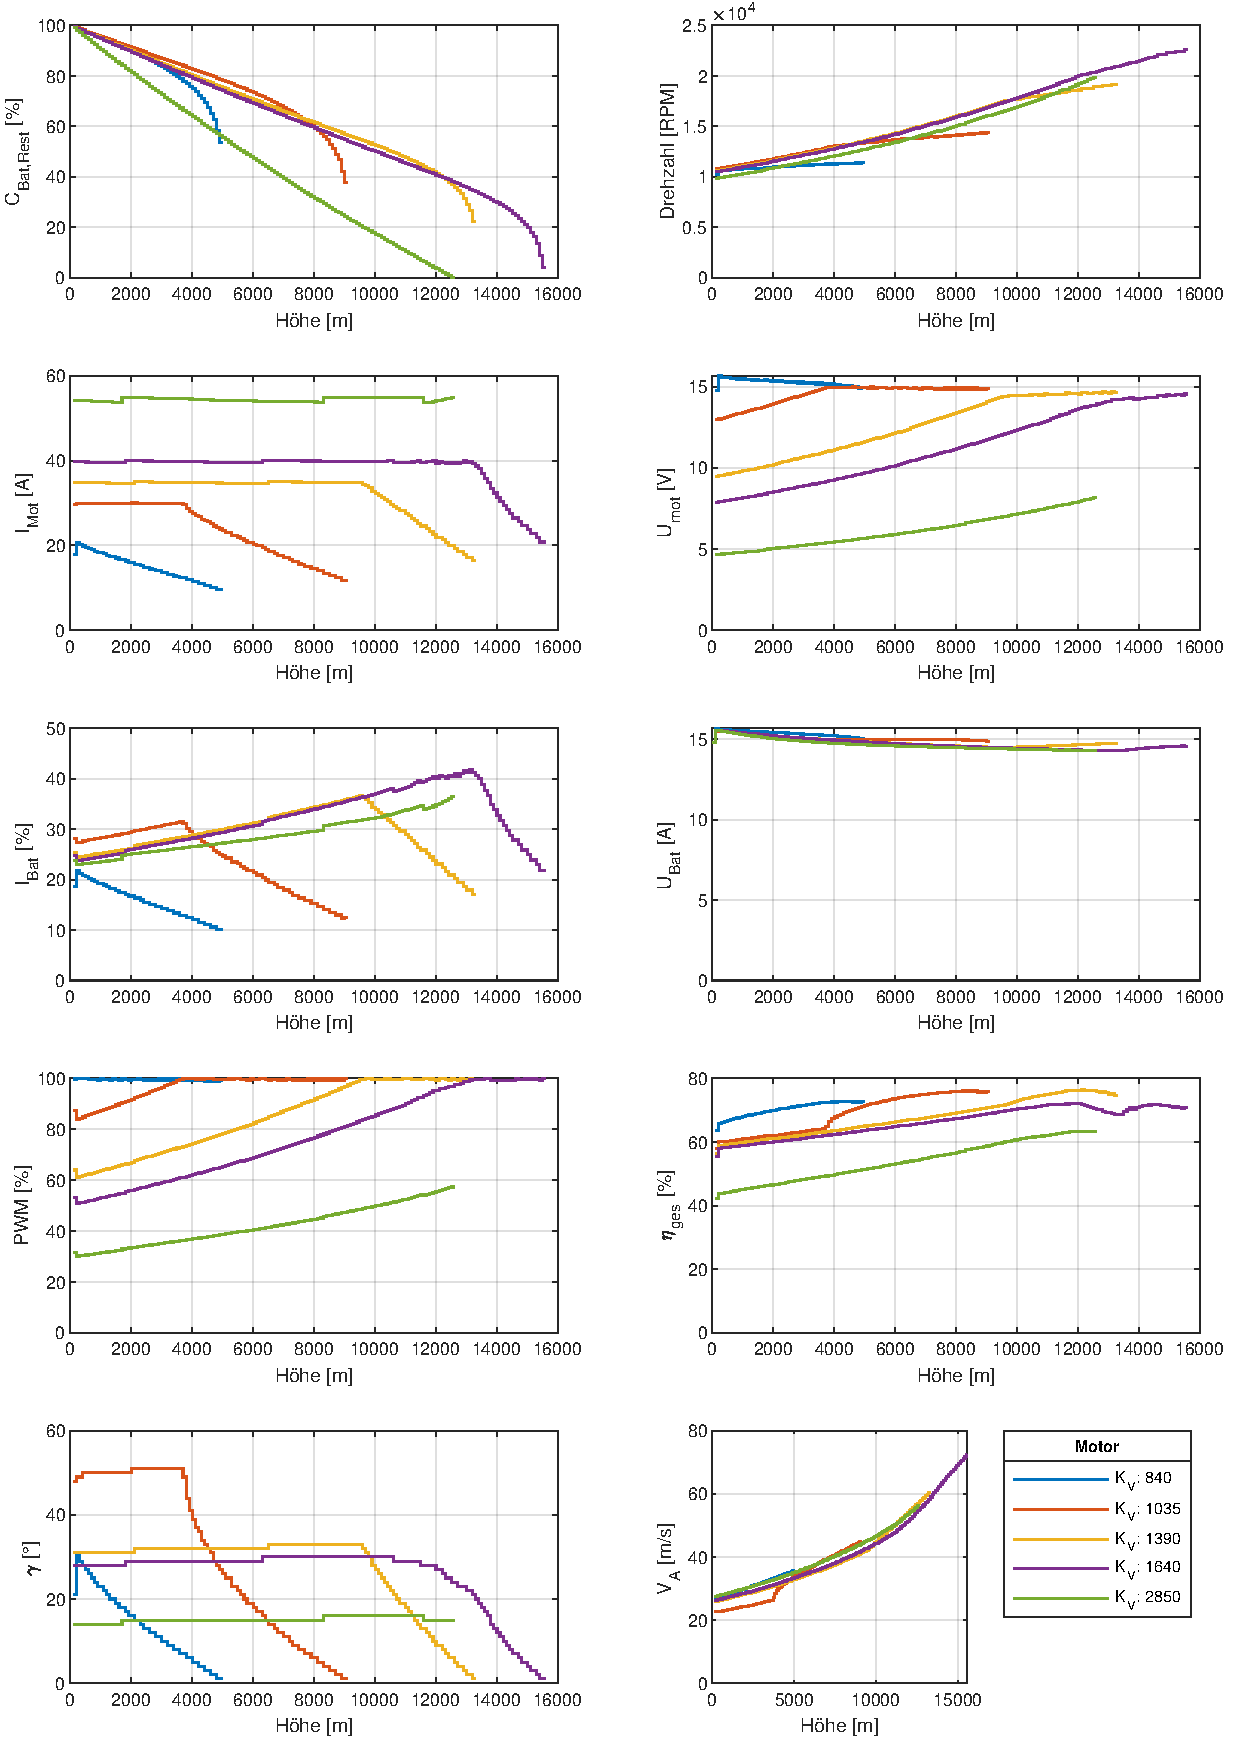
\includegraphics[scale=0.7]{Diagramme/Flaechenflzg_Mot_Prop.pdf}
	\caption{Einfluss der Motor-Propeller-Kombination auf die Flugleistungen der Flächenflugzeug-Referenzkonfiguration (Tab. \ref{tab:referenzkonfiguration})}
	\label{abb:flaechenflzg_mot_prop}
\end{figure}

Der \ensuremath{K_V}-Wert ist ein Kennwert für die Anzahl der Umdrehungen pro Minute pro Volt im Leerlauf. Ein hoher \ensuremath{K_V}-Wert bedeutet nun im Umkehrschluss, dass bei einer hohen Drehzahl die Spannung geringer ist als für einen Motor mit einem vergleichsweise niedrigem \ensuremath{K_V}-Wert. Die Drehzahl ist in diesem Fall für fast alle Motoren identisch bzw. die Unterschiede minimal. Gleichzeitig sinkt allerdings das Verhältnis von Drehmoment pro Ampere, das der \ensuremath{K_M}-Wert ausdrückt  \cite[S.35 und S.42-43]{Buchi.2013}. Es gilt die Beziehung
\begin{equation}
	K_M = 1/K_V\cdot 30/\pi \eqend{.}
\end{equation}
Ein Motor mit hohem \ensuremath{K_V}-Wert muss daher einen hohen Dauermotorstrom besitzen, um gute Flugleistungen zu erzielen (Vgl. Abb. \ref{abb:flaechenflzg_mot_prop}). Durch diese Abhängigkeit wird auch die PWM beeinflusst. Der Motor mit einem \ensuremath{K_V} von \SI{840}{RPM/V} erreicht durch seine hohe Motorspannung deutlich schneller das Niveau der Batteriespannung und hat somit seinen Leistungsüberschuss aufgebraucht. Somit wird auch frühzeitiger das Absinken des Bahnneigungswinkels eingeleitet. Für Motoren mit einem niedrigeren \ensuremath{K_V}-Wert bedeutet dies auch gleichzeitig das Ende des Steigfluges. Wieder anders ist dieser Zusammenhang für Motoren mit einem hohen \ensuremath{K_V}-Wert. Hier wird \SI{100}{\%} PWM erst bei deutlich größeren Höhen erreicht oder gar nicht, weshalb folglich der optimale Bahnneigungswinkel erst später nicht mehr gehalten werden kann und danach sinkt. Bei \ensuremath{\gamma = \SI{0}{^\circ}} ist der Steigflug beendet. Hierbei steigt zudem der optimale Bahnneigungswinkel mit dem \ensuremath{K_V}-Wert. Da die Geschwindigkeit mit einem höheren Bahnneigungswinkel sinkt (Vgl. Gleichung \ref{eq:geschw_flaechenflugzeug}), sinkt auch die benötigte Leistung, die hauptsächlich für die Motoren mit geringem \ensuremath{K_V} begrenzend ist. Dabei nimmt die Restladung für kleinere \ensuremath{K_V}-Werte nicht so schnell ab wie dies für große der Fall ist. Dies kann auf den höheren Gesamtwirkungsgrad und im Detail auf den höheren Motorreglerwirkungsgrad zurückgeführt werden. Durch die deutlich höhere Pulsweitenmodulation ist der Wirkungsgrad des Motorreglers entsprechend höher (Vgl. Gleichung \ref{eq:eta_pwm}). Außerdem sind die Verluste durch Temperatur  sowie Innenwiderstand oder Leerlaufstrom für einen Motoren mit niedrigem \ensuremath{K_V}-Wert geringer. Der letzte starke Anstieg des Gesamtwirkungsgrades für \SI{840}{RPM/V} und \SI{1035}{RPM/V} liegt am Propellerwirkungsgrad. Durch den starken und schnellen Abfall des Bahnneigungswinkels steigt entsprechend die Fluggeschwindigkeit \ensuremath{V_A} signifikant an (Vgl. Gleichung \ref{eq:geschw_flaechenflugzeug}). Als Konsequenz auf den starken Anstieg der Fluggeschwindigkeit steigt auch der Propellerwirkungsgrad (Vgl. Gleichung \ref{eq:eta_prop}). \\
Zusammengefasst besitzen Motoren mit einem niedrigen \ensuremath{K_V}-Wert eine erhöhte Effizienz im Betrieb, die sich gegenüber mit einem höheren \ensuremath{K_V} vor allem in der Abnahme der Restladung widerspiegelt. Allerdings ist die Leistung unzureichend für den in dieser Arbeit geforderten Aufstieg. Dies macht sich vor allem im Leistungsüberschuss bemerkbar. Ein zu hoher \ensuremath{K_V}-Wert des Motors bedeutet auf der anderen Seite jedoch wieder zu hohe Verluste und somit erneut eine nicht optimale Konfiguration des Flächenflugzeugs. Folglich liegt das Optimum in der Mitte der beiden Grenzen. Es ist also ein Motor mit einem hohen \ensuremath{K_V}-Wert zu wählen, der aber auch geringe interne Verluste und Verluste im Motorregler aufweist. Dies wird gut durch den hier verwendeten Motor mit 1390 \ensuremath{K_V} repräsentiert. \\
%Hier sei auch nochmal auf den Sprung im Verlauf der Leistungsgrößen für die Motoren mit 1390 und 1640 \ensuremath{K_V} hingewiesen. Da dieser bei beiden an der gleichen Stelle auftritt und die Drehzahlverläufe komplett identisch sind, kann dieser auf eine Inkonsistenz im Propellerkennfeld zurückgeführt werden.



\subsection{Anzahl der Motoren und Propeller}
\label{subsec:anz_mot_flaechenflzg}
Während die Leistung der Motoren mit gleichem Gewicht schon einen großen Einfluss auf den optimalen Steigwinkel hat, ändert sich dies bedeutend mit der Anzahl der Motoren (Vgl. Abb. \ref{abb:flaechenflzg_n_prop}). Schon mit einer Steigerung der Motorenanzahl auf 2 verändert sich der optimale Steigwinkel zu \SI{90}{^\circ}. Die dazu zugehörige Steiggeschwindigkeit liegt hierbei beim Maximum der Iterationsweite von der Steiggeschwindigkeit (siehe Abschn. \ref{subsubsec:schub_flaechenflzg}).
Auch hier kann die Effektivität und Effizienz einer Propelleranzahlerhöhung wieder an dem Diagramm der Restladung festgemacht werden. Je mehr Propeller verwendet werden, desto schneller sinkt die Restladung auf \SI{0}{\%}. Dies ist für alle Konfigurationen bis auf die Referenzkonfiguration der Fall, die ihre Dienstgipfelhöhe erreicht. Mit Ausnahme für zwei Propeller sinkt mit steigender Anzahl der Propeller auch die maximal erreichbare Höhe. Der Schub ist für alle Konfigurationen ähnlich, jedoch wird dieser bei einer Propelleranzahl von mehr als eins auf die Propeller aufgeteilt. Damit sinkt die erforderliche Leistung pro Motor. Dies macht sich in einer Verringerung der Drehzahl bemerkbar, die in einer Verringerung des Motorstroms (siehe Gleichung \ref{eq:motorstrom}) und der Motorspannung (Vgl. Abb. \ref{eq:motorspannung}) mündet. Diese erhöhen in Summe allerdings auch den Batteriestrom (Vgl. Gleichung \ref{eq:batteriestrom}) und führen zu einem stärkeren Einbruch der Batteriespannung. Rückwirkend durch die geringe Motorspannung fällt auch die PWM äußerst niedrig aus (Vgl. Gleichung \ref{eq:pwm}), was den ESC-Wirkungsgrad \ensuremath{\eta_{PWM}} durch größere Verluste verschlechtert (Vgl. Gleichung \ref{eq:eta_pwm}). Der geringe Schub pro Propeller in Kombination mit der geringen Drehzahl vermindern den Propellerwirkungsgrad \ensuremath{\eta_{Prop}} (Vgl. Gleichung \ref{eq:eta_prop}), der zusammen mit dem ESC-Wirkungsgrad den Gesamtwirkungsgrad \ensuremath{\eta_{ges}} verringert.\\
Alle Flächenflugzeugkonfigurationen mit \ensuremath{n_{Prop}} größer eins haben gemeinsam, dass bis ca. \SI{9000}{m} Höhe ein Steigflug mit \SI{90}{^\circ} den effizientesten Steiglfug bestimmt. 
Dies ist solange der optimale Betriebspunkt bis der Steigwinkel von \SI{55}{^\circ} ab ca. \SI{8500}{m} energieeffizienter ist. Ein vergleichbares Flugverhalten ist bei einer Erhöhung der Anzahl auf 4 zu beobachten. Dies repräsentiert das Verhalten eines VTOL-Flugzeuges, dass mit \ensuremath{\gamma = 90^\circ} vertikal startet und ab \SI{9000}{m} Höhe in die Transition auf einen Bahnneigungswinkel von \SI{55}{^\circ} übergeht. 
Bemerkenswerter Weise sind die Kurven der Restladung von einem und zwei Propellern deckungsgleich, obwohl alle übrigen Leistungsparameter signifikant unterschiedliche Werte aufzeigen durch die veränderte Propelleranzahl und das durch den zusätzlichen Motor erhöhte Gewicht des Flächenflugzeugs. Dies bedeutet, dass der Vorteil der Schubhalbierung und der vertikale Steigflug gerade den Nachteil des zusätzlichen Motorgewichts kompensiert. Der zweite Übergang in den vertikalen Steigflug ab \SI{16500}{m} stellt einen ineffizienten Flugzustand dar, was vor allem durch den Verlauf der Restladung und des Gesamtwirkungsgrades reflektiert wird. Ein Grund für den Übergang liegt in dem verringerten Widerstand im vertikalen Steigflug. Dieser entspricht nur noch dem Nullwiderstand (vgl. Gleichung \eqref{eq:widerstand_vertikalflug}). Für einen Steigflug mit einem Bahnneigungswinkel \ensuremath{\gamma} von weniger als \SI{90}{^\circ} wächst der Widerstand quadratisch mit der progressiv ansteigenden Geschwindigkeit (vgl. Gleichung \eqref{eq:geschwindigkeit_skalierung}).\\
Insgesamt verringert eine Erhöhung der Motor- und Propelleranzahl um zwei den TOC um ca. \SI{7500}{m}. Die optimale Propelleranzahl ist in diesem Fall zwei, weil mit dieser Anzahl die Dienstgipfelhöhe in weitere Höhen verschoben wird.
(Der kurze Sprung bei \ensuremath{n_{Prop} = 6} wird in der Untersuchung vernachlässigt).

\begin{figure}[H]
\centering
	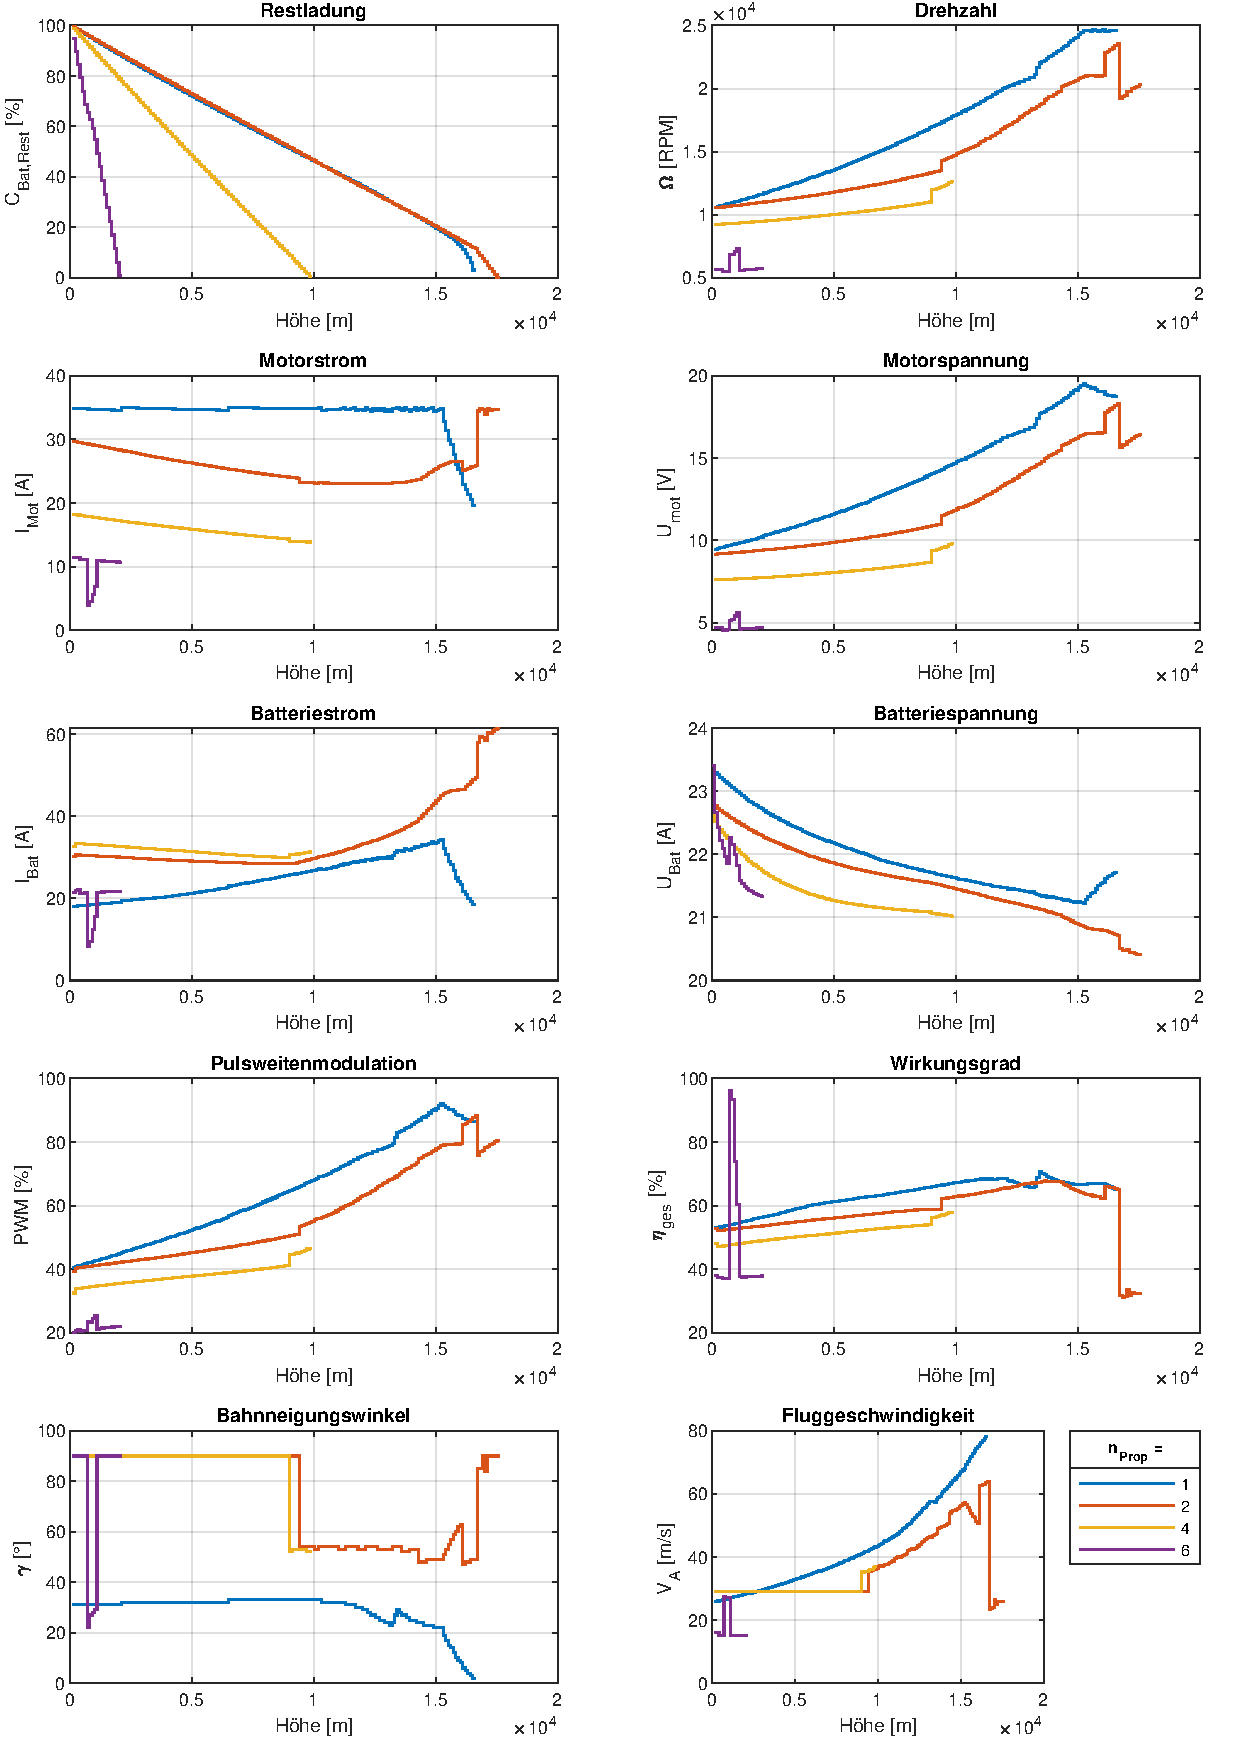
\includegraphics[scale=0.7]{Diagramme/Flaechenflzg_n_prop.pdf}
	\caption{Einfluss der Propelleranzahl auf die Flugleistungen der Flächenflugzeug-Referenzkonfiguration (Tab. \ref{tab:referenzkonfiguration})}
	\label{abb:flaechenflzg_n_prop}
\end{figure}


\subsection{Gleitzahl}
\label{subsec:gleitzahl}
Der Einfluss der Gleitzahl äußert sich hauptsächlich in Effizienz des Flächenflugzeugkonfiguration, die wiederum durch die Abnahme der Restladung ausgedrückt wird (vgl. Abb. \ref{abb:gleitzahl})
Alle Verläufe erreichen die Dienstgipfelhöhe, die durch die maximale Propellerdrehzahl \ensuremath{\Omega_{Prop}} limitiert wird. Ohne diese limitierende Höhe könnte das Flächenflugzeug bei linearer Extrapolation der Restladungskurve sogar mit einer Gleitzahl von 50 eine Höhe von ca. \SI{25000}{m} erreichen. 
Mit einer Verringerung der Gleitzahl geht auch eine Verringerung der maximalen Höhe mit einher und umgekehrt. Eine entsprechend hohe Gleitzahl bedeutet gleichzeitig auch eine hohe aerodynamische Güte (Vgl. \cite[S.34]{Scheiderer.2008}). Dazu sinkt der Widerstand im Vergleich zum Auftrieb, sodass für ein Flächenflugzeug mit einer höheren Gleitzahl (Vgl. Gleichung \ref{eq:gleitzahl}) für den gleichen Auftrieb weniger Leistung zur Kompensation des Widerstandes aufgebracht werden muss. Als Konsequenz dessen steht mehr Leistung für das Steigen zur Verfügung. Mit der Gleitzahl steigt ebenso der optimale Bahnneigungswinkel. Als Grund dafür kann wieder die verringerte Widerstandsleistung angeführt werden. Zusätzlich sinkt die Zeit zum Überwinden einer Höhendifferenz mit einem steileren Winkel. Einen Änderung der Gleitzahl hat nur einen Einfluss auf die Restladung, die Batteriespannung und den Bahnneigungswinkel. Eine geringe Gleitzahl bedeutet einen stärkeren Einbruch der Batteriespannung, da wiederum für den gleichen Auftrieb mehr Widerstand kompensiert werden muss. \\
Auffällig ist noch die Flugleistungsverbesserung mit der Gleitzahl. Diese macht sich im Verlauf der Restladung deutlich bemerkbar. Eine Verbesserung der Gleitleistung von \ensuremath{E = 4} auf \ensuremath{E = 6} bedeutet auf einer Höhe von \SI{15000}{m} bereits \SI{10}{\%} mehr Restladung und einen \SI{7}{^\circ} höheren Bahnneigungswinkel. Eine erneute Erhöhung der Gleitzahl auf 10 steigert die Restladung auf dieser Höhe über dem  Meereslevel nur noch um \SI{5}{\%} und eine Erhöhung des Bahnneigungswinkel \SI{5}{^\circ}. Dieser Trend der abnehmenden Flugleistungsoptimierung bei einer gleichzeitigen Verdoppelung der Gleitleistung setzt sich fort (siehe \ref{abb:gleitzahl}).
Das einfache Flächenflugzeugmodell berücksichtigt nicht, dass eine Gleitzahlerhöhung auch mit einer deutlichen Erhöhung der Strukturmasse einhergeht, weil die Flugzeugzelle, die Flügelform, das Flügelprofil usw. an die neuen Bedingungen angepasst und verstärkt werden müssen. Dieser Zusammenhang wird beim Vergleich der Gleitleistung eines Segelflugzeugs mit dessen Spannweite deutlich. \\
Dementsprechend ist eine Erhöhung des Penalty-Faktors zwingend erforderlich. Unter Berücksichtigung dieser Zusammenhänge gilt es einerseits die Gleitleistung des Flächenflugzeugs für eine Verbesserung der Flugleistungen zu steigern, dies auf der anderen Seite mit der zusätzlichen Masse der Flugzeugstruktur und dem tatsächlichen Gewinn an Flugleistungen abzuwägen. Es ist zu mutmaßen, dass eine Gleitzahl zwischen 6 und 10 die besten Ergebnisse erzielt.

\begin{figure}[H]
\centering
	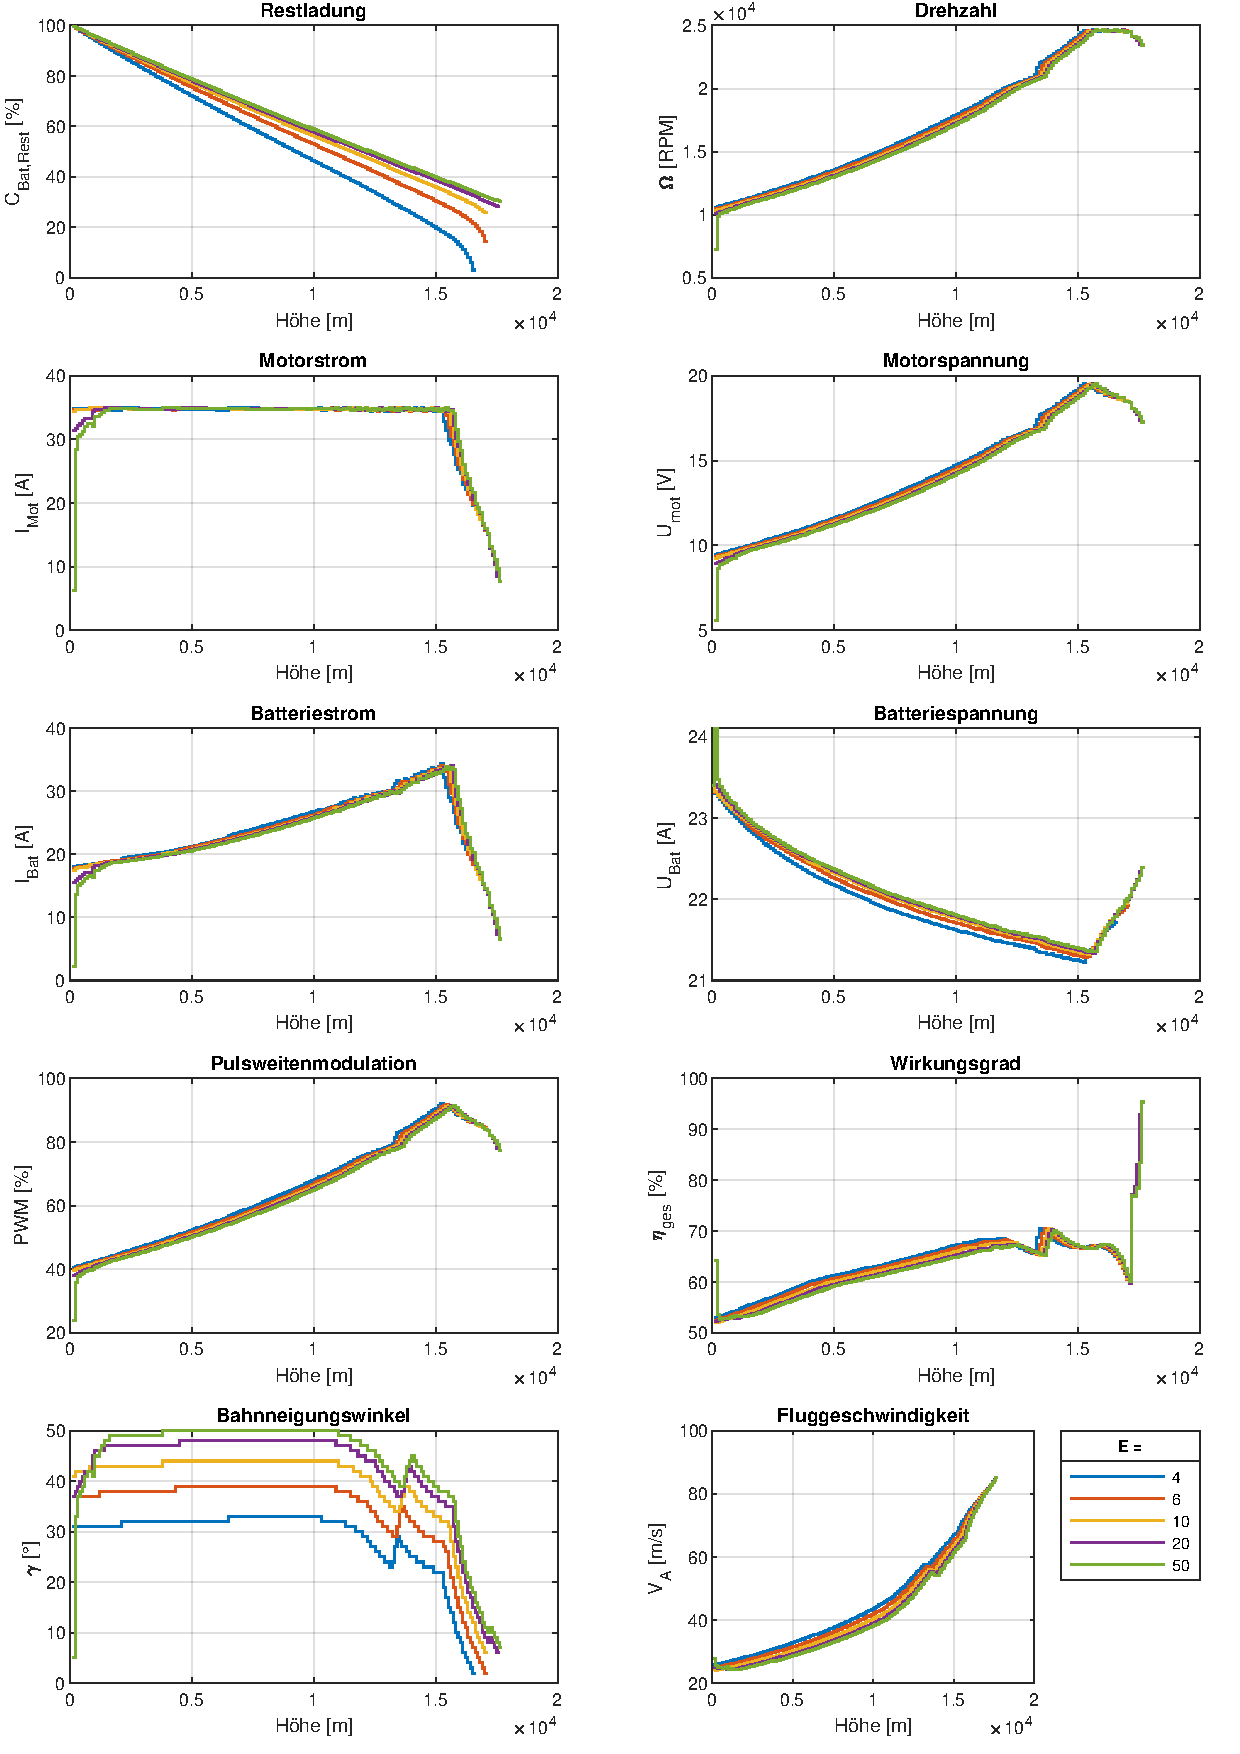
\includegraphics[scale=0.7]{Diagramme/Flaechenflzg_E.pdf}
	\caption{Einfluss der Gleitzahl auf die Flugleistungen der Flächenflugzeug-Referenzkonfiguration (Tab. \ref{tab:referenzkonfiguration})}
	\label{abb:gleitzahl}
\end{figure}


\subsection{Auslegungsgeschwindigkeit}
\label{subsec:vstern}
Die Auslegungsgeschwindigkeit ruft ähnlich zu der Motor-Propeller-Kombination (vgl. Abb. \ref{abb:flaechenflzg_mot_prop}) oder Propelleranzahl (vgl. Abb. \ref{abb:flaechenflzg_n_prop}) Einflüsse auf das Leistungsverhalten des Flächenflugzeugs hervor. Da für den Steigflug ein Flug mit konstantem Auftriebsbeiwert vorausgesetzt wird, erhöht sich aufgrund dessen die Fluggeschwindigkeit mit der Höhe und größerem Bahnneigungswinkel (Vgl. Gleichung \ref{eq:geschw_flaechenflugzeug}).
Ist die Auslegungsgeschwindigkeit gering, so wächst sie absolut gesehen mit der Höhe nicht so stark wie bei hohen Auslegungsgeschwindigkeiten (Vgl. Verlauf der Fluggeschwindigkeit über der Höhe in Abb. \ref{abb:vstern}). 
Bis zu einem \ensuremath{V^\star} von \SI{75}{km/h} ist die Batterierestladung der limitierende Faktor für die Flughöhe. Ab einer Auslegungsgeschwindigkeit von \SI{100}{km/h}, die auch diejenige der Referenzkonfiguration ist, wird wieder die Dienstgipfelhöhe durch \ensuremath{Ma_{tip} = 1} an der Propellerblattspitze erreicht. Bis zu einer Höhe von \SI{13000}{m} sind auch die Verläufe der Restladung von \ensuremath{V^\star} mit \SI{100}{km/h} und \SI{125}{km/h} identisch. Für alle Auslegungsgeschwindigkeiten ist das Flugverhalten gleich dem aus Abschn. \ref{sec:multicopter_vs_flaechenflugzeug}. Es wird wieder solange mit maximalen Motorstrom geflogen, bis entweder die Restkapazität \SI{0}{\%} erreicht oder die Dienstgipfelhöhe durch einen anderen limitierenden Leistungsparameter, in diesem Fall wieder die Propellerdrehzahl, erreicht ist. Durch die höhere Auslegungsgeschwindigkeit und demzufolge auch die höhere Fluggeschwindigkeit (vgl. Gleichung \ref{eq:geschw_flaechenflugzeug}) kommt es zu einer höheren Propelleranströmgeschwindigkeit. Um trotzdem den gleichen Schub zu erzeugen ist eine höhere Drehzahl notwendig. Mit dem schneller drehenden Propeller steigt auch die Motorspannung (vgl. Gleichung \eqref{eq:motorspannung}), der Batteriestrom und über die Motorspannung auch die PWM. Die gesteigerte Propelleranströmgeschwindigkeit verbessert den Propellerwirkungsgrad und als Konsequenz daraus den Gesamtwirkungsgrad. Daher ist der Gesamtwirkungsgrad für größere Auslegungsgeschwindigkeiten besser. Dies kann auch auf den verbesserten Motorreglerwirkungsgrad bei einer höheren PWM zurückgeführt werden (vgl. Gleichung \ref{eq:eta_pwm}). Es kann schließlich noch festgehalten werden, dass mit steigender Auslegungsgeschwindigkeit der Bahnneigungswinkel \ensuremath{\gamma} abnimmt, da die Zeit zum Überwinden eines Höhenschritts bei einer höheren Geschwindigkeit und geringerem Bahnneigungswinkel sich kaum ändert. \\
Aufgrund dieser Tatsachen ist das Flächenflugzeug auf einigermaßen hohe Fluggeschwindigkeiten von rund \SI{100}{km/h} auszulegen, um zum einen den Leistungsüberschuss der Motoren ausreichend hoch zu halten und zum anderen die Zeit zum Aufstieg nicht zu vergrößern. Weiterhin wird die Auslegungsgeschwindigkeit durch die Wahl des Propellers beeinflusst. Bei gleichem Durchmesser steigt die optimale Auslegungsgeschwindigkeit mit der Propellersteigung.

%Eine geringer gewählte Auslegungsgeschwindigkeit im Horizontalflug bedeutet daher auch, dass länger mit maximalen Motorstrom geflogen werden kann, bevor die Motorspannung die Batteriespannung erreicht und somit das Absinken des Steigwinkels einleitet (vgl. Abb. \ref{abb:vstern}).
%Da mit der Auslegungsgeschwindigkeit auch die Geschwindigkeit mit der Höhe steigt, sind für hohe Geschwindigkeiten Propeller mit hohem Pitch vom Vorteil.
%Ein Optimum zeichnet sich bei \SI{75}{km/h} aus. Es kann festgehalten werden, dass mit der Auslegungsgeschwindigkeit der Bahnneigungswinkel abnimmt, da die Steigzeit bei einer höheren Geschwindigkeit und geringerem Bahnneigungswinkel sich kaum ändert. Außerdem wird schneller \SI{100}{\%} PWM erreicht und damit gleichzeitig die Motorspannung begrenzt und der Flug mit maximalen Motorstrom beendet. Außerdem nimmt mit der Motorspannung der Zuwachs der Propellerdrehzahl ab. Weiterhin ist ein Zuwachs des Gesamtwirkungsgrades sowie der Bahngeschwindigkeit zu verzeichnen. Bei hohen Geschwindigkeiten begrenzt der mögliche Steigwinkel \ensuremath{\gamma} den Steigflug im Gegensatz zu der Begrenzung durch die Restladung bei niedrigen Auslegungsgeshwindigkeiten. Das schnelle Absinken von \ensuremath{\gamma} am Ende des Steigfluges durch aufgebrauchten Leistungsüberschuss bedeutet für alle Auslegungen einen ineffizienten Flugzustand, da damit die Flugzeit für eine Höhenschritt ansteigt und folglich auch eine deutlich höhere Energieentnahme der Batterie mit sich zieht.

\begin{figure}[H]
\centering
	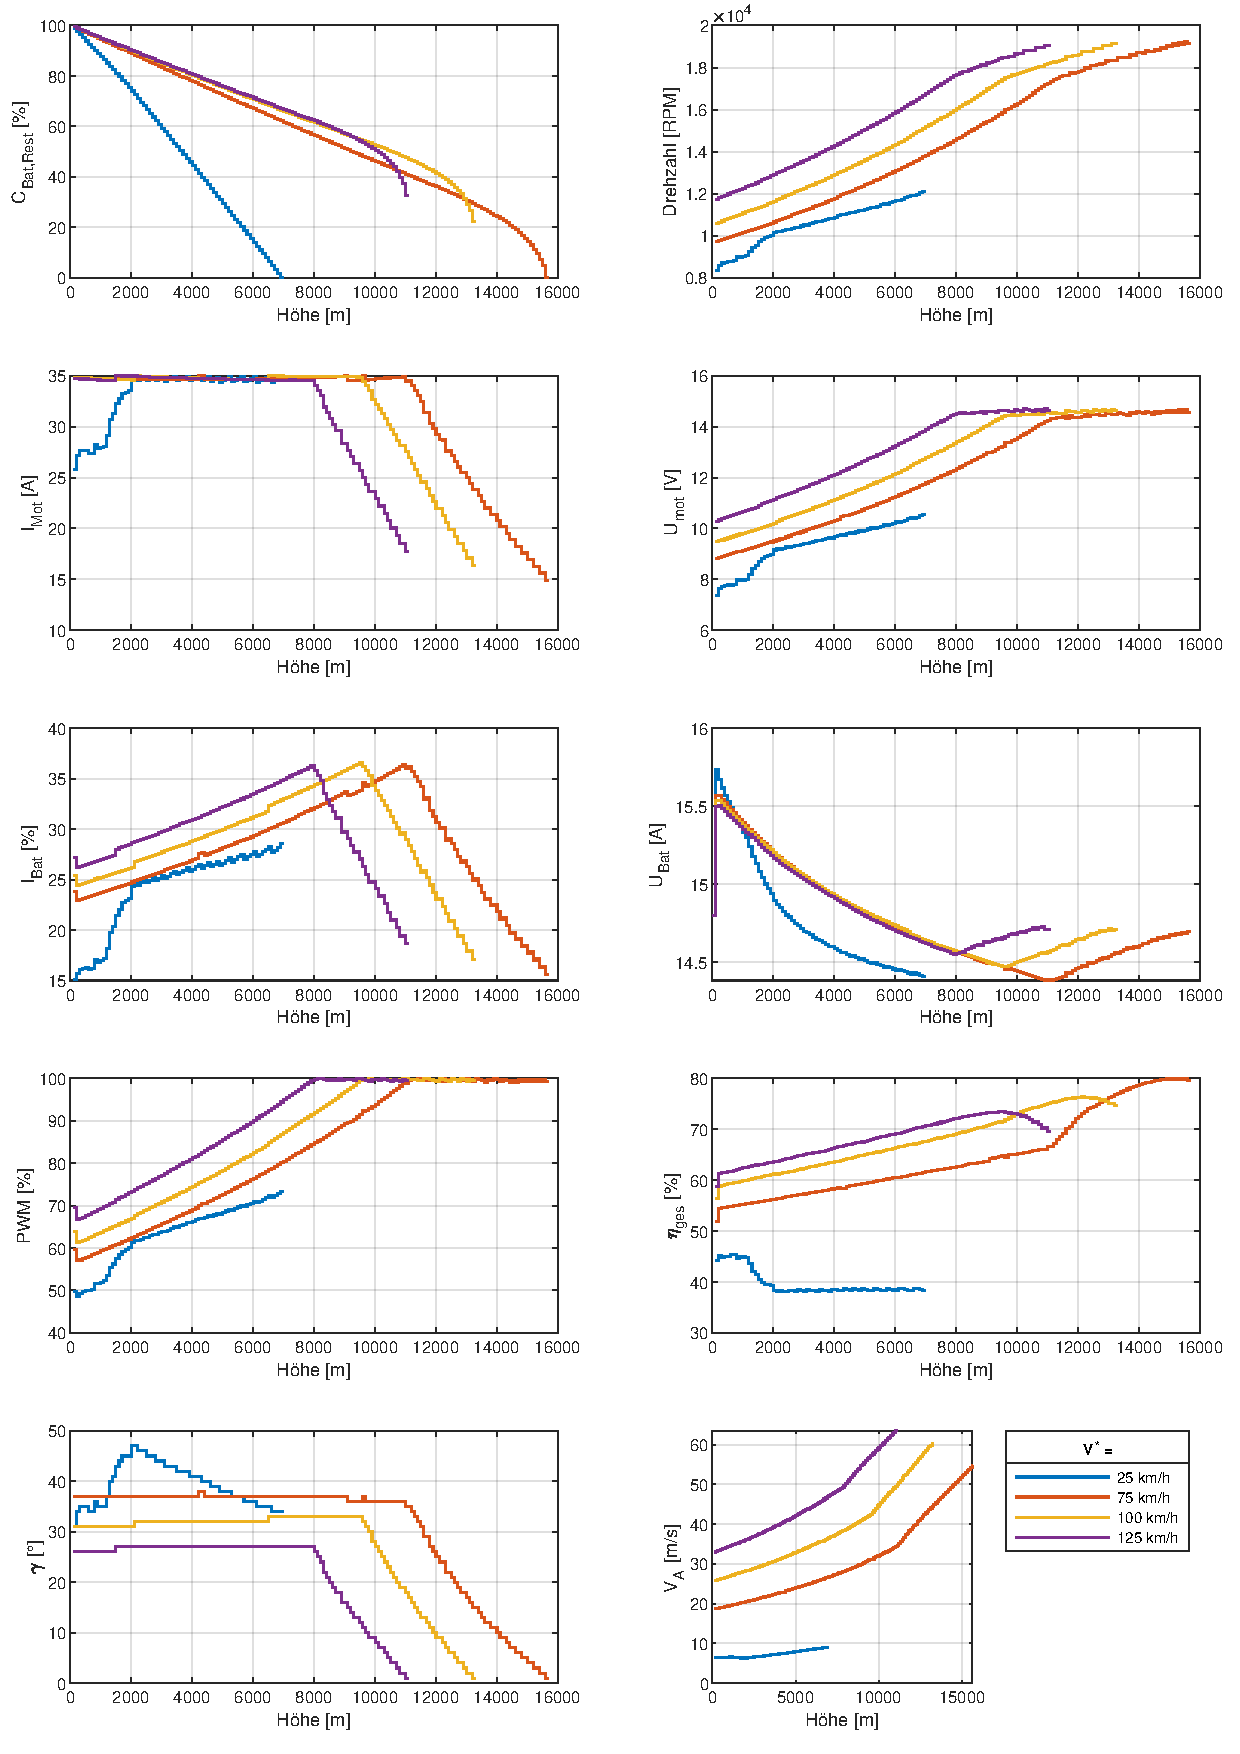
\includegraphics[scale=0.7]{Diagramme/Flaechenflzg_Vstern.pdf}
	\caption{Einfluss der Auslegungsgeschwindigkeit auf die Flugleistungen der Flächenflugzeug-Referenzkonfiguration (Tab. \ref{tab:referenzkonfiguration})}
	\label{abb:vstern}
\end{figure}



\subsection{Penalty-Faktor}
\label{subsec:f_p}
Beim Vergleich von einem Flächenflugzeug mit einem Multicopter muss bei gleichem Gesamtgewicht die unterschiedliche Verteilung der Gewichtskomponenten berücksichtigt werden. Für ein Flugzeug ist das Strukturgewicht von Flügeln und Rumpf sowie den Steuerungselementen bedeutend größer als das von einem Multicopter. Ein Penaltyfaktor von 1 entspricht daher wie oben beschrieben einer optimistischen Einschätzung, wenn beide Strukturgewichte bei einem gleichen Gesamtgewicht äquivalent sind. Um realistischere Ergebnisse für ein Flächenflugzeug zu erreichen, wird der Penaltyfaktor schrittweise erhöht. Dabei verringert sich auch die maximal erreichbare Höhe.
Der Einfluss des Penalty-Faktors konzentriert sich auf die Restladung und die Batteriespannung (vgl. Abb. \ref{abb:fp}). Dies hängt damit zusammen, dass ein Penalty-Faktor größer als 1 die zur Verfügung stehende Batteriemasse (vgl. Gleichung \ref{eq:penalty}) und folglich die Batteriekapazität (vgl. Gleichung \ref{eq:batteriekapazitaet}) reduziert. Die Referenzkonfiguration mit \ensuremath{f_P = 1} ist die einzige Konfiguration, die bis zur Dienstgipfelhöhe aufsteigt. Bei allen anderen nimmt die Restladung vorher \SI{0}{\%} an. Die Gesamtmasse ist unabhängig vom Penalty-Faktor identisch für jede Konfiguration, weshalb auch der Schub der gleiche ist und alle übrigen Verläufe der Leistungsparameter identisch sind. 
Aufgrund der Tatsache, dass die Batteriekapazität mit der Batteriemasse abnimmt, der Batteriestrom jedoch gleich bleibt, wird die Entladerate bezogen auf die Kapazität größer (vgl. Gleichung \ref{eq:c_rate}). Dies ist der Grund für den zunehmenden Spannungsabfall der Batterie bei einem höheren Penalty-Faktor.\\
Insbesondere in Bezug auf Abschn. \ref{subsec:gleitzahl} ist der Penalty-Faktor von Bedeutung. Einer Anpassung der Flächenflugzeugzelle in Richtung einer Flugleistungsverbesserung sind Grenzen gesetzt. 


\begin{figure}[H]
\centering
	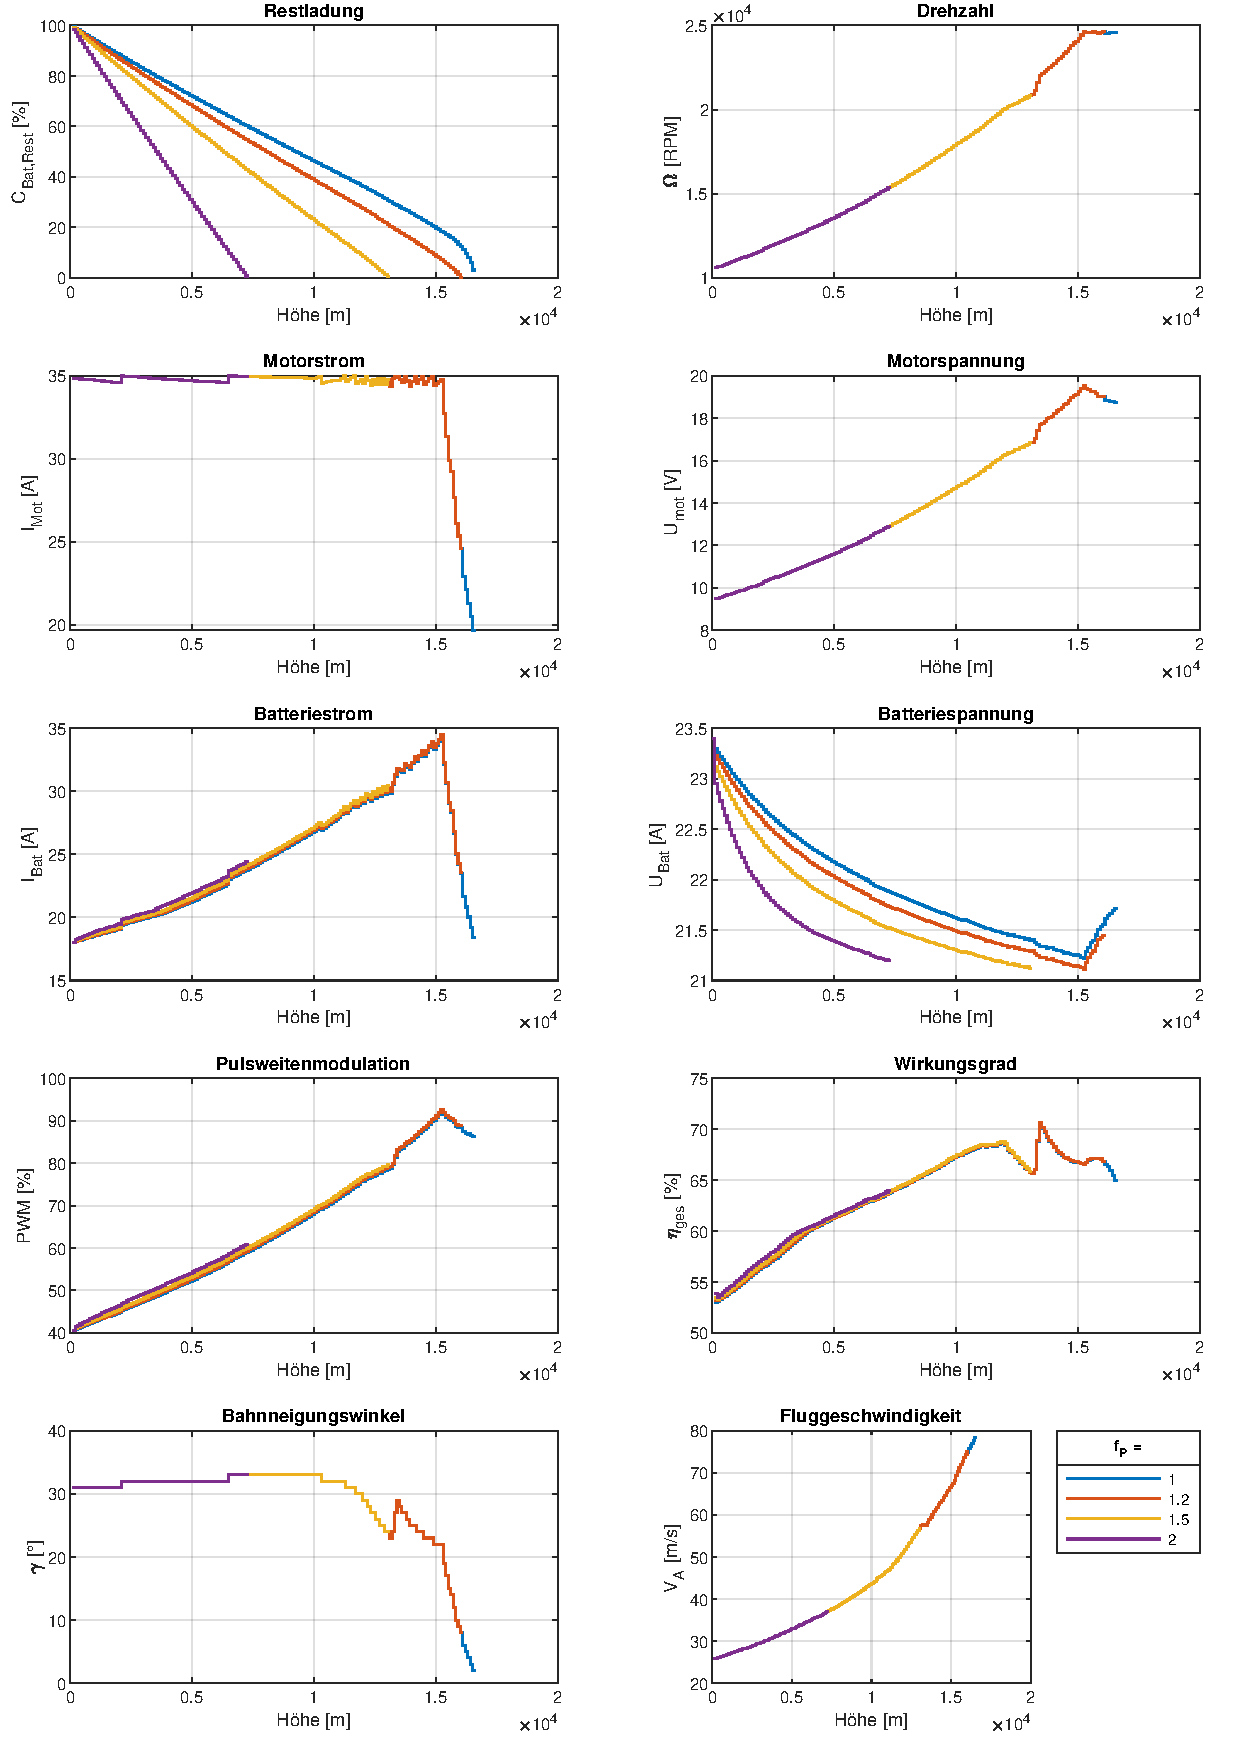
\includegraphics[scale=0.7]{Diagramme/Flaechenflzg_fp.pdf}
	\caption{Einfluss des Penalty-Faktors auf die Flugleistungen der Flächenflugzeug-Referenzkonfiguration (Tab. \ref{tab:referenzkonfiguration})}
	\label{abb:fp}
\end{figure}

\subsection{Zusammenfassung}
Aus den Ergebnissen wird ersichtlich, dass es viele Einflussfaktoren auf die Flugleistungen eines Flächenflugzeug für einen Steigflug auf \SI{10}{km} oder sogar \SI{15}{km} Höhe gibt. Zuerst sollte ein Motor mit einem vergleichsweise hohem \ensuremath{K_V}-Wert in seiner Gewichtsklasse gewählt werden, wobei der Propeller an den Motor anzupassen ist (vgl. Abschn. \ref{subsec:mot_prop_kombi}). Zur Vermeidung transsonischer Effekte sollte der Propellerdurchmesser entsprechend groß gewählt werden, was auch für die Steigung gilt. Die optimale Anzahl der Propeller liegt bei einem oder zwei. Je nach der Propelleranzahl variiert der effizienteste Bahnneigungswinkel, sodass bei einer Propelleranzahl von mindestens zwei das Flächenflugzeug als VTOL-Fluggerät am effizientesten fliegt (vgl. Abschn. \ref{subsec:anz_mot_flaechenflzg}). Weiterhin ist die Gleitleistung so groß wie möglich zu halten (vgl. Abschn. \ref{subsec:gleitzahl}). Hierbei sind einer solchen Erhöhung durch den Penalty-Faktor Grenzen gesetzt (vgl. Gleichung \ref{subsec:f_p}). Die Auslegungsgeschwindigkeit ist an den Propeller anzupassen und so hoch wie möglich zu wählen, um einen Kompromiss aus verbesserter Steiggeschwindigkeit und verringerter Schuberzeugung durch den Propeller zu finden (vgl. Abschn. \ref{subsec:vstern}). In diesem Rahmen ist die Referenzkonstruktion bereits sehr gut ausgelegt.\\


\section{Ergebnisse des Vergleichs} 
Im direkten Vergleich weist das Flächenflugzeug eine größere maximale Flughöhe (vgl. z.B. Abb. \ref{abb:referenzkonfiguration}) auf als der Quadrocopter aus \cite{Anderson.2018}. Besonders mit hohen Gleitzahlen (vgl. Abschn. \ref{subsec:gleitzahl}), mehreren Motoren (vgl. Abschn. \ref{subsec:anz_mot_flaechenflzg}) und einer guten Kombination aus Motor und Propeller (vgl. Abschn. \ref{subsec:mot_prop_kombi}) wird dieser Vorteil ersichtlich. Jedoch vernachlässigt das einfache Modell des Flächenflugzeugs zusätzliche Widerstände. Die Vorteile eines Flächenflugzeuges zeigen sich auch nur bei einem Penalty-Faktor nahe eins. Dies muss als unrealistisch angesehen werden. Besonders im Bezug auf eine hohe Gleitzahl geht diese Anforderung mit einer hohen Flügelstreckung und damit mit einem hohen Strukturgewicht einher. Somit ist es zwingend notwendig den Penalty-Faktor zu erhöhen. Werden diese Einschränkungen berücksichtigt, schwindet der zusätzliche Höhengewinn eines Flächenflugzeugs gegen Null. Weiterhin erweist sich das Flächenflugzeug als bereits in den möglichen Maßen im Rahmen dieses Modells als optimiert. Die Steiggeschwindigkeit ist in Bezug auf den Auslegungszustand und einem Flug bei Auslegungsgleitzahl optimal. Außerdem wird der Steigwinkel für jeden Höhenabschnitt optimiert (vgl. Abschn. \ref{subsubsec:schub_flaechenflzg}) und eine gute Kombination von Motor und Propeller ist bereits gegeben (vgl. Abschn. \ref{sec:multicopter_vs_flaechenflugzeug}). Schlussendlich ist damit der Spielraum für weitere Verbesserungen eingeschränkt. Ohne die Limitierung durch den Propeller könnte ein  ideales Flächenflugzeug Höhen von mehr als \SI{18000}{m} erreichen. \\
Hingegen zeigt der Quadrocopter in dieser Hinsicht noch Potential. Ein zu untersuchender Punkt ist noch die Abkehr von einer konstanten Steiggeschwindigkeit hin zu einer kontinuierlichen Optimierung mit der Höhe. %Das Flächenflugzeugmodell aus Abschn. \ref{subsubsec:schub_flaechenflzg} vernachlässigt hier die Abhängigkeit des Flugzeugentwurfs von der Masse. Jede Designänderung verändert die Konstruktion des Flächenflugzeugs z.B. die Struktur und dessen Stärke, das Fahrwerk, den Motor und so weiter. Dieser Zusammenhang findet in dem Flächenflugzeugmodell nur durch die Wahl des Penalty-Faktors Berücksichtigung. \\
Wird für das Flugzeug außerdem eine Konstellation von mehr als einem Motor gewählt, neigt das Flugzeug dazu in einem \SI{90}{^\circ} Winkel zu steigen (vgl. Abschn. \ref{subsec:anz_mot_flaechenflzg}). Damit zeigt sich die optimale Flugweise in einem vertikalen Steigflug. Hierbei werden nichtsdestotrotz wieder viele Vereinfachungen getroffen und Verluste nicht berücksichtigt. 
In der Berechnung der Flächenflugzeugaerodynamik bleibt der Einfluss von Seitenwinden unberücksichtigt, da Seitenwinde nur die Strecke über Grund beeinflussen nicht aber die Flugeigenschaften im Steigflug (siehe Kap. \ref{subsubsec:schub_flaechenflzg}). Unter Berücksichtigung an das angedachte Operationsziel, einer Atmosphärenmessung, sind die Flugkorridore, die von der Deutschen Flugsicherung (DFS) zur Verfügung gestellt werden, begrenzt. Daher ist eine Abdrift bei sehr hohen Seitenwinden für die Mission negativ und muss vom Fluggerät ausgeglichen werden. Dies verbraucht zusätzlich Energie zum Ausgleichen und reduziert nochmals die erreichbare Höhe. Das geschieht beim Quadrocopter bereits durch den Ausgleich der Seitenwinde mit einer Anpassung vom Winkel \ensuremath{\alpha_{M}}, also einer Schrägstellung der Rotorebene. Ein weiteres Argument, was gegen den Einsatz von einem Flächenflugzeug spricht ist, dass eine Start und Landevorrichtung von Nöten ist. Das erfordert Platz für eine Start- und Landebahn. Aufgrund seiner Senkrechtstarterfähigkeit benötigt der Multicopter wenig Platz zum Starten und Landen. 
Entsprechend dieser Argumentation wird in dieser Arbeit entschieden, dass ein Multicopter gegenüber einem Flächenflugzeug für einen Steigflug in die untere Stratosphäre als vorteilhaft anzusehen ist.


%******************************************************************
\newpage
\section{Einflussfaktoren auf den Quadrocopter}
\label{sec:steiggeschwindigkeit}
Eine weitere Optimierung des Multicopters bzw. des Quadrocopters kann durch eine Anpassung der Steiggeschwindigkeit geschehen. Die vormalig als konstant angenommene Steiggeschwindigkeit von \SI{10}{m/s} (Kap. \ref{chap:nachbildung_des_quadrocopter}) ist nicht in jedem Operationspunkt optimal. Die Steiggeschwindigkeit wird wieder für jeden Höhenschritt variiert (siehe Anhang \ref{sec:vvar_vorgehen}). Analog zur Variation des Steigwinkels beim Flächenflugzeug fällt die Auswahl der Geschwindigkeit auf den Wert, welcher die geringste Energiemenge benötigt für den Aufstieg. Bei der Untersuchung kristallisieren sich drei starke Einflussfaktoren heraus. Im Einzelnen sind das der Widerstandsbeiwert, die Anzahl der Batteriezellen und die Motorleistung. Im Anhang \ref{abb:steiggeschw} ist der Ablauf der Leistungsberechnung für die Steiggeschwindigkeit dargestellt. In diesem Abschnitt werden die oben genannten Parameter an der Konstellation aus Kap. \ref{chap:nachbildung_des_quadrocopter} untersucht, da dies den Einfluss sehr gut verdeutlicht.


\subsection{Einfluss der Steiggeschwindigkeit auf den Quadrocopterflug}
Im folgenden soll der Einfluss einer optimierten Bahngeschwindigkeit aufgezeigt werden. Um die Optimierung besonders hervorzuheben, wird sie auf den Quadrocopter aus Kap. \ref{chap:nachbildung_des_quadrocopter} angewandt. 
Durch die Optimierung der Steiggeschwindigkeit ist ein zusätzlicher Höhengewinn von \SI{1000}{m} im Vergleich zu dem Flug mit konstanter Bahngeschwindigkeit von \SI{10}{m/s} zu vermerken. Bei dem neuen TOC auf \SI{14100}{m} wird allerdings die Dienstgipfelhöhe erreicht. Ohne diese Limitierung und bei linearer Extrapolation Restladungskurve könnte der Quadrocopter bei Verwendung eines anderen Propellers eine Höhe von \SI{17000}{m} erreichen. Die Flugleistungen sind nicht durch die Motorleistung begrenzt sondern durch die Maximaldrehzahl des Propellers. Diese ist auf \SI{17000}{RPM} festgelegt. Ein Grund dafür kann in der Festigkeit des Propellers gefunden werden. Nichtsdestotrotz ist ein Flug mit variierbarer Steiggeschwindigkeit signifikant effizienter. Dies macht sich deutlich in der Restladung bemerkbar. Die Abnahme der Restladung ist pro Höhenschritt geringer als in Kap. \ref{sec:ergebnisse_quadrocopter}. Auf \SI{10260}{m} sind noch \SI{40}{\%} Restladung vorhanden. Das entspricht ca. \SI{10}{\%} mehr Restladung in der gleichen Höhe wie in Kap. \ref{chap:nachbildung_des_quadrocopter}. Die Propellerdrehzahl steigt beinahe sofort auf ihr Maximum von \SI{17000}{RPM} an und verbleibt auf diesem Niveau bis zum TOC. Rückwirkend ist damit auch der Motorstrom ab \SI{4000}{m} auf dem Niveau der Batteriespannung und somit die PWM auf \SI{100}{\%}. Der Leistungsüberschuss ist gleich null. Dieser Zustand ist auch durch ein Maximum der Bahngeschwindigkeit gekennzeichnet mit \SI{30}{m/s}. Die Bahngeschwindigkeit ist damit dreimal so hoch. Der Motorstrom \ensuremath{I_{Mot}} sinkt im Laufe des Fluges immer weiter ab. Da die Drehzahl konstant bleibt, die Dichte aber mit der Höhe abnimmt, sinkt auch das Drehmoment an der Motorwelle und letztlich der Motorstrom (vgl. Gleichung \ref{eq:motorstrom}). Über den Motorstrom sinkt die Motorspannung ebenfalls leicht ab (vgl. Gleichung \ref{eq:motorspannung}), weil die Drehzahl auf einem konstanten Niveau bleibt. Während die Batteriespannung von \SI{16}{V} auf \SI{15}{V} durch die Last einbricht, fällt mit der Motorspannung auch die PWM unterhalb von \SI{100}{\%}. Die Bahngeschwindigkeit steigt zuerst auf ihr Maximum  sinkt danach kontinuierlich auf \SI{0}{m/s}. Somit wird die Dienstgipfelhöhe erreicht. Die Flugzeit kann auf die Bahngeschwindigkeit zurückgeführt werden. Bereits nach \SI{13}{min} und \SI{20}{sec} wird der TOC erreicht. \\
Der Motorreger verzeichnet wenige Verluste durch die hohe PWM und besitzt deshalb einen hohen Wirkungsgrad. Der Propellerwirkungsgrad steigt am Anfang durch den Drehzahlanstieg (vgl. Gleichung \ref{eq:eta_prop}) und ebenso mit dem Schub und der Bahngeschwindigkeit. Während der Schubüberschuss aufgebraucht ist, sinkt mit der Höhe die Dichte und dementsprechend der Schub. Mit dem Schub sinkt auch die leistungstechnisch mögliche Bahngeschwindigkeit, was einen starken Einbruch im Propellerwirkungsgrad hervorruft.

\begin{figure}[H]
\centering
	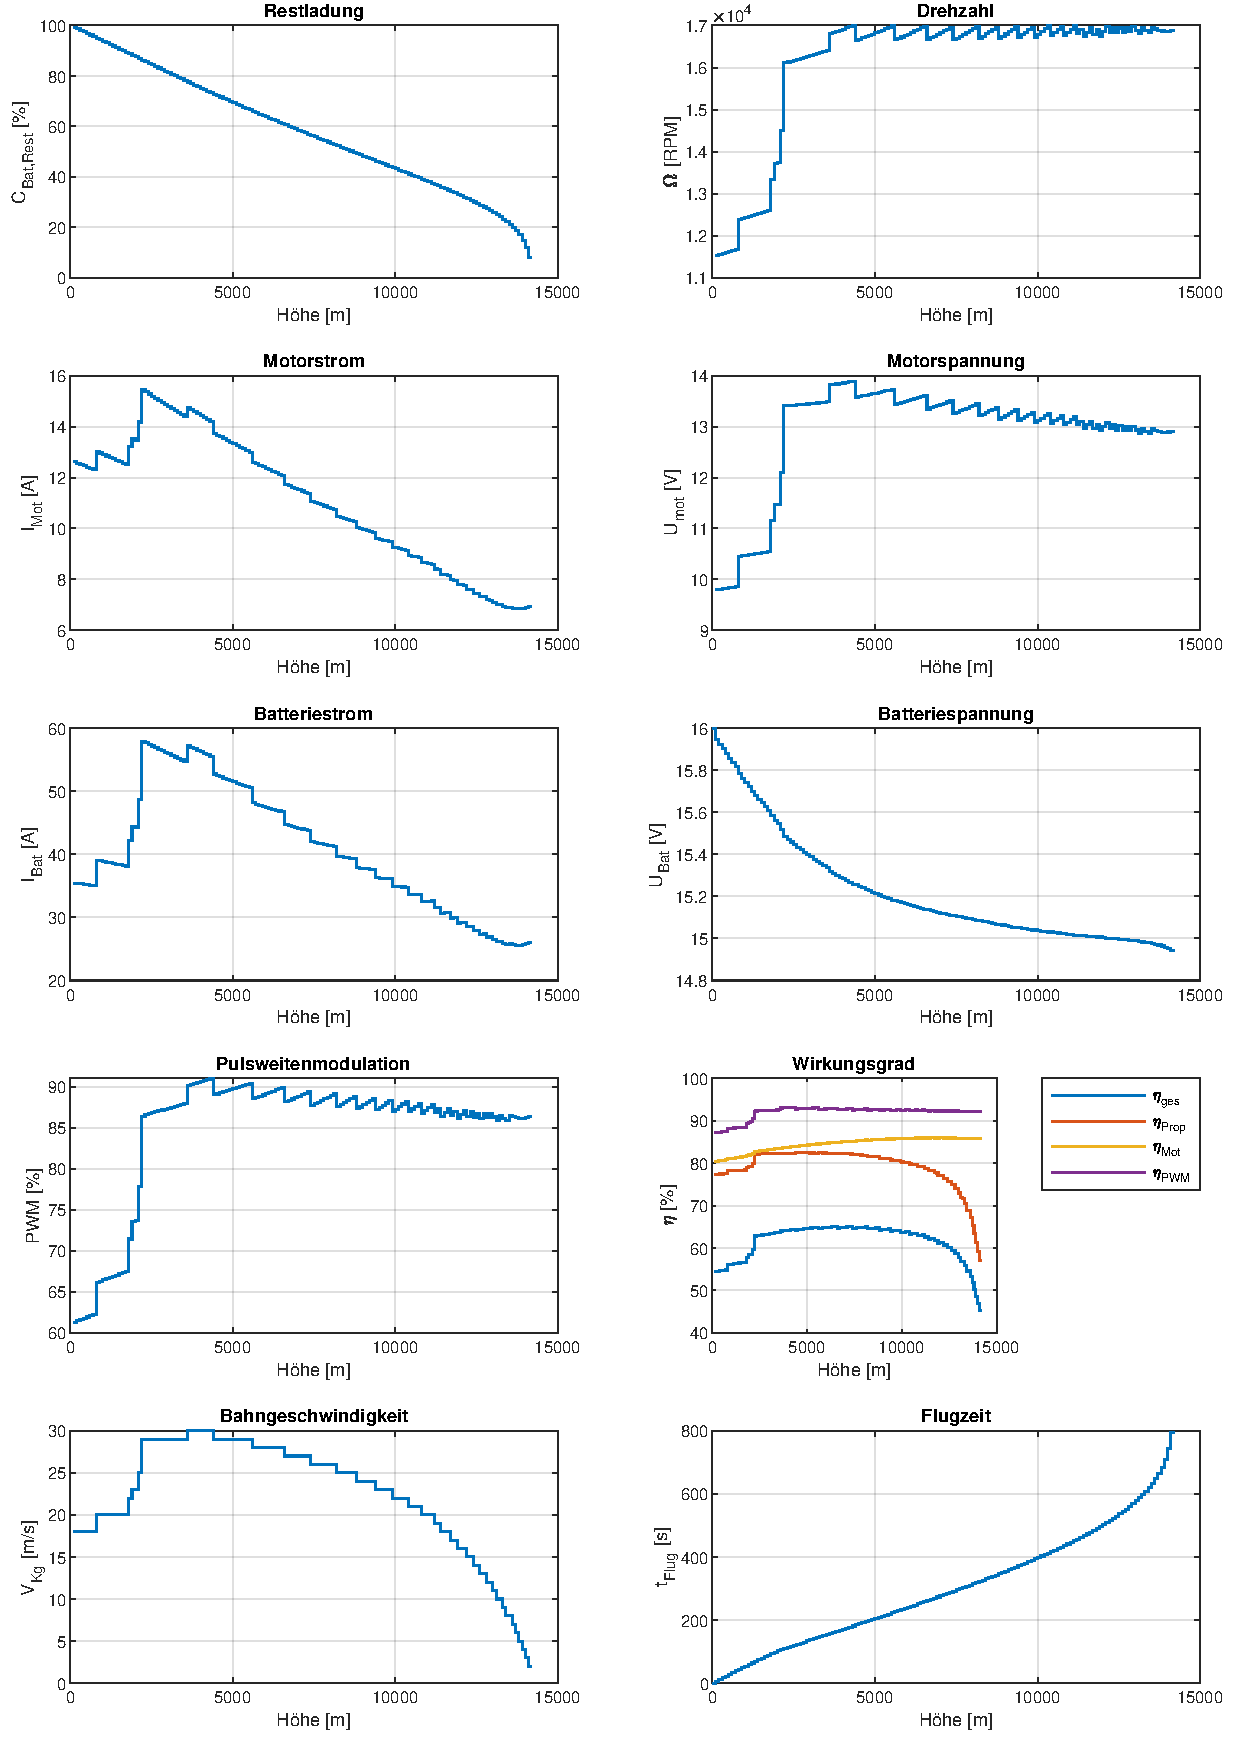
\includegraphics[scale=0.7]{Diagramme/Russland_vvar.pdf}
	\caption{Flugleistungen des Quadrocopter aus \cite{Anderson.2018} mit variabler Steiggeschwindigkeit}
	\label{abb:russland_vvar}
\end{figure}

Im Folgenden soll analog zum Flächenflugzeug eine Referenzkonfiguration für einen Multicopter in Tab. \ref{tab:referenzkonfiguration_mulitcopter} festgelegt werden.

\begin{center}
	\captionof{table}{wichtige Parameter der Multicopter-Referenzkonfiguration}
	\begin{tabular}{l l l} \hline
		Parameter & Variablenname & verwendete Größe \\ \hline
		Gesamtmasse \ensuremath{m} & \texttt{m} & \SI{3,078}{kg} \\
		Leermasse des Multicopters \ensuremath{m_{copter}}& \texttt{m\_copter} & \SI{1.028}{kg} \\ 
		Batteriemasse \ensuremath{m_{Bat}} & \texttt{m\_Bat} & \SI{1,626}{kg} \\
		Motormasse \ensuremath{m_{Mot}}& \texttt{m\_Mot} & \SI{106}{g} \\
		Geschwindigkeitskonstante \ensuremath{K_V} & \texttt{K\_V} & \SI{1390}{RPM/V} \\
		maximaler Dauerstrom \ensuremath{I_{max}} & \texttt{I\_max} & \SI{35}{A} \\
		Propeller & \texttt{prop\_name} & 11x3 \\
		Anzahl Propeller \ensuremath{n_{Prop}} & \texttt{n\_prop} & \SI{4}{} \\ 
		Anzahl der Batteriezellen \ensuremath{N_{Bat,cell}} & \texttt{N\_bat\_cell} & 6 \\	 
		Obere Stirnfläche \ensuremath{F_{copter,oben}} & \texttt{F\-copter\_oben} & \SI{0,0209}{m^2} \\
		Oberer Widerstandsbeiwert \ensuremath{c_{W,copter,oben}} & \texttt{c\_W\_copter\_oben} & 1 \\ \hline
	\end{tabular}	
	\label{tab:referenzkonfiguration_mulitcopter}
\end{center}

Die Umgebungsparameter sind die für eine Normatmosphäre auf Meereshöhe (entspr. QNH). Dazu wurde der Seitenwind nicht wie im AEROMET\_UAV Projekt auf \SI{100}{km/h} sondern auf konstante \SI{10}{m/s} festgesetzt. Der Grund hierfür ist, dass der Leistungsüberschuss in einem mäßig schnellen Vorwärtsflug am größten ist \cite[S.328-S.329]{Wall.2015}. Dieser Zusammenhang wird mit der Windgeschwindigkeit modelliert. Außerdem kann der Einfluss einzelner Parameter besser und genauer untersucht werden. Die AEROMET\_UAV Randbedingungen werden später in Kap. \ref{sec:aeromet_rb} berücksichtigt.


\subsection{Einfluss des Widerstands}
\label{subsec:widerstandseinfluss}
Der Widerstandsbeiwert hat einen Einfluss auf die Flugleistungen eines Multicopters, der als gering eingeschätzt werden kann (vgl. Abb. \ref{abb:c_W_einfluss}). Unabhängig von dem Widerstandsbeiwert \ensuremath{c_W} endet für alle Konfigurationen der Steigflug bei der Dienstgipfelhöhe. Auch hier stellt die Prepellerdrehzahl den die Höhe limitierenden Parameter dar, die ab \SI{20100}{RPM} eine Blattspitzengeschwindigkeit \ensuremath{Ma_{tip}} von \ensuremath{Ma = 1} erreicht. Das Erreichen der Dienstgipfelhöhe wirkt sich jedoch kaum auf die Restladung aus.
Die Flugzustände sind dieselben wie in Abschn. \ref{sec:multicopter_vs_flaechenflugzeug}. Bis zu einer Höhe von \SI{15000}{m} erfolgt der Steigflug bei maximalen Motorstrom \ensuremath{I_{max}}. Mit dem Schub und der abnehmenden Dichte steigt die Drehzahl, die in einer Erhöhung der Motorspannung mündet. Durch die Belastung fällt die Batteriespannung ab, sodass diese in Kombination mit der Motorspannung in einer PWM Erhöhung resultiert. Nach einem anfänglichen Anstieg auf ca. \SI{52,5}{\%} fällt der Gesamtwirkungsgrad \ensuremath{\eta_{ges}} auf \SI{41,5}{\%} ab. 
Am deutlichsten kann der Einfluss des Widerstandsbeiwertes an dem Verlauf der Restladung und der Bahngeschwindigkeit ausgemacht werden. 
Bei einem großen maximalen Motorstrom gilt, dass die Begrenzung der Geschwindigkeit durch den Widerstandsbeiwert erfolgt. Eine sehr hohe Geschwindigkeit verringert zum einen die Flugzeit für einen Höhenschritt, erhöht auf der anderen Seite jedoch den Widerstand und damit zusätzlich die benötigte Leistung (vgl. Gleichung \ref{eq:widerstand}). Je geringer der \ensuremath{c_W} gewählt wird, desto höher ist die optimale Steiggeschwindigkeit. Erhöht sich im Umkehrschluss der Luftwiderstand so sinkt die Steiggeschwindigkeit, da der Widerstand mit der Geschwindigkeit quadratisch (vgl. Gleichung \ref{eq:widerstand}) ansteigt. Zudem erhöht ein geringer Widerstandsbeiwert die vorhandene Restkapazität. Anhand der Restkapazitätsabnahme kann ein beinahe lineare Abhängigkeit zwischen einer \ensuremath{c_W}-Erhöhung und einer Abnahme der Restladung festgestellt werden. Im Schnitt sinkt mit einer Anhebung des \ensuremath{c_W}-Wertes um 0,5 die Restladung auf \SI{15000}{m} um \SI{4}{\%}. Im Vergleich zum Einfluss der Gleitzahl auf die Flugleistungen eines Flächenflugzeuges ist der Verlauf hier ähnlich. 
Im Sinne einer großen maximalen Höhe ist daher eine aerodynamisch günstige Verkleidung des Multicopters anzustreben.
  
\begin{figure}[H]
\centering
	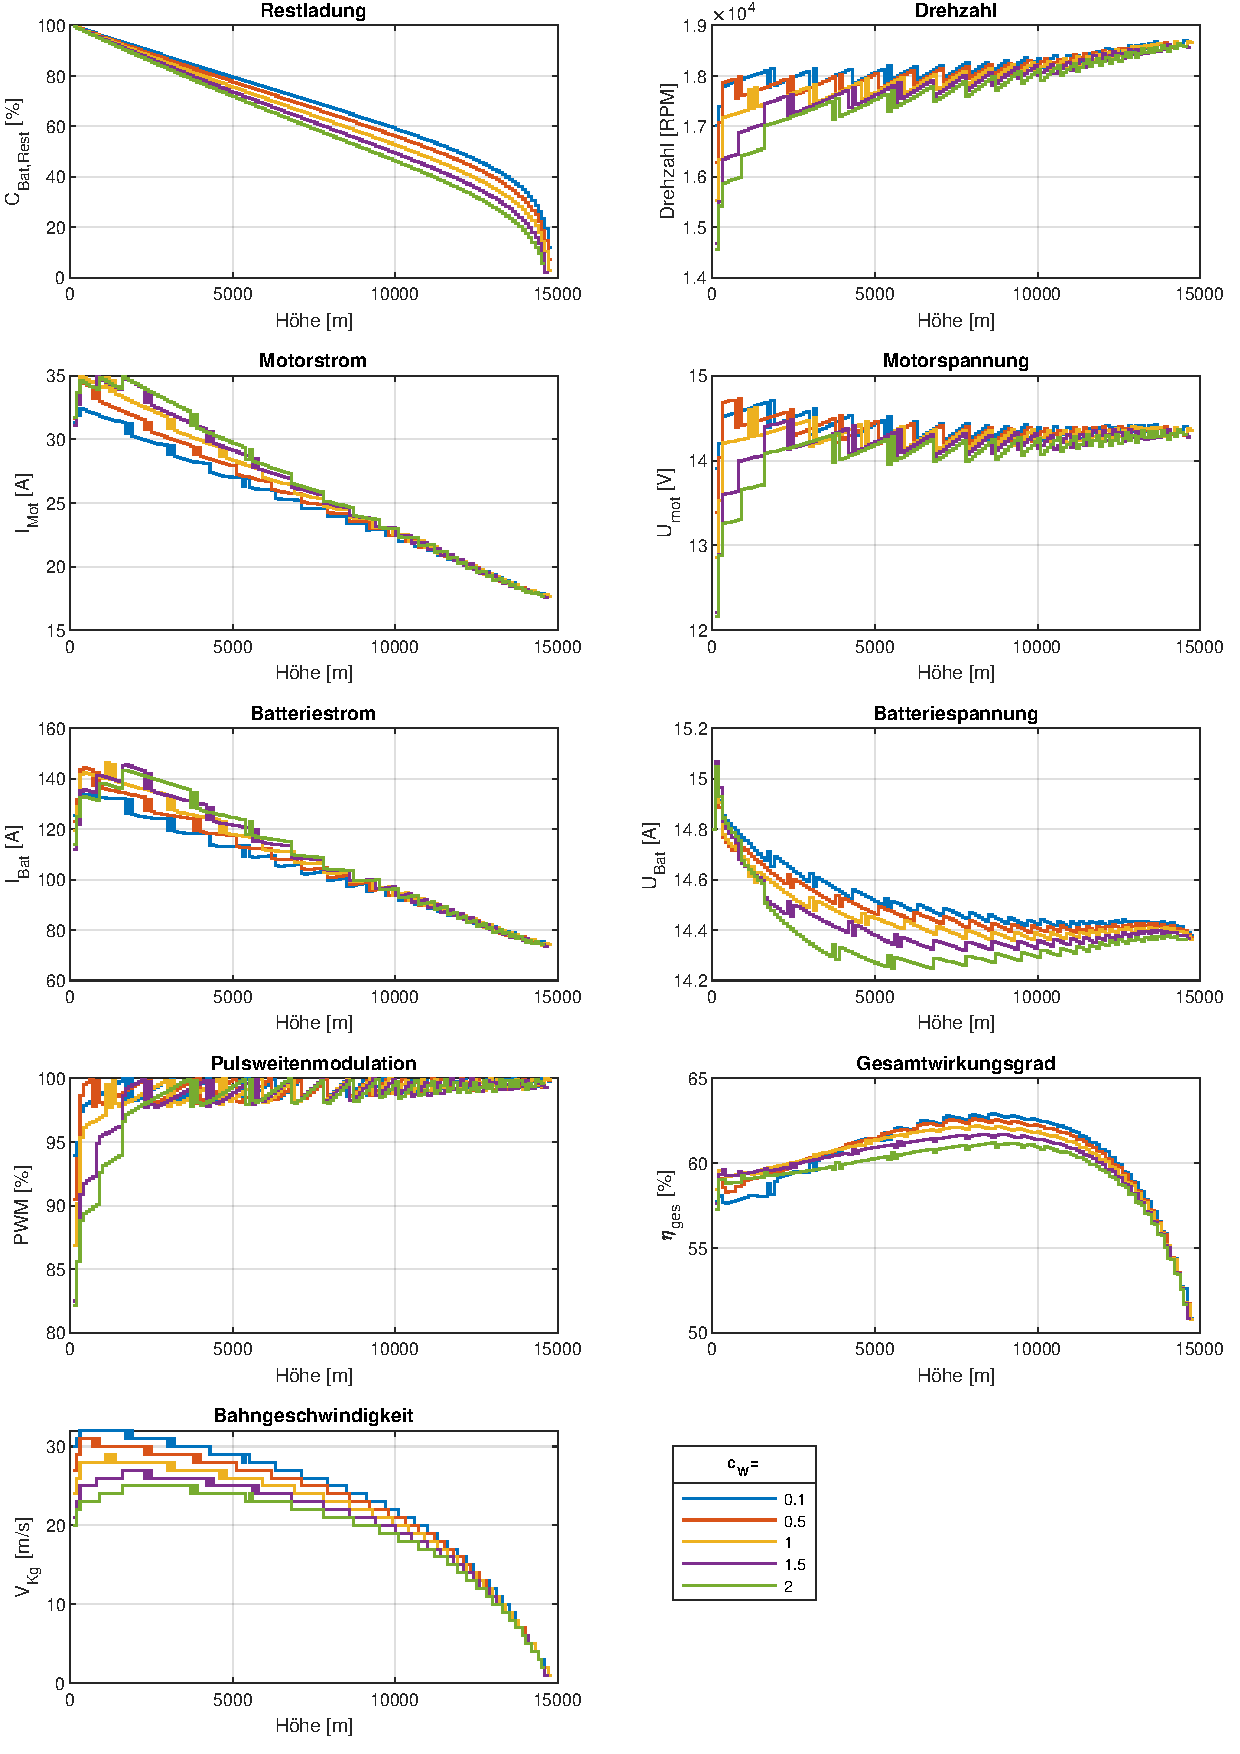
\includegraphics[scale=0.7]{Diagramme/Untersuchung_c_W.pdf}
	\caption{Einfluss des Widerstandsbeiwertes auf die Flugleistungen der Multicopter-Referenzkonfiguration (Tab. \ref{tab:referenzkonfiguration_mulitcopter})}
	\label{abb:c_W_einfluss}
\end{figure}


\subsection{Einfluss der Batteriespannung}
\label{subsec:einfluss_n_bat}
Wie in Kap. \ref{subsec:mot_prop_kombi} gezeigt, ist ein weiterer begrenzender Parameter die max. Motorleistung bzw. die PWM. Die Motorspannung an sich kann nicht beeinflusst werden. Jedoch lässt sich Einfluss auf die Höhe der Motorspannung durch eine Erhöhung der in Reihe geschalteten Batteriezellen nehmen. Mit jeder zusätzlichen Zelle erhöht sich die nominelle Batteriespannung um \SI{3,7}{V} (vgl. Abb. \ref{abb:N_Bat_einfluss}). Damit stellt die PWM nicht mehr die Grenze für die Steiggeschwindigkeit dar. Der effizienteste Flugzustand ist nun der beim maximalen, dauerhaften Motorstrom. Jedoch führt bei gleicher Energiemenge und somit gleicher Masse 
\begin{equation}
	E_{Bat} = C_{Bat}\cdot U_{Bat}
\end{equation}
eine Erhöhung der Spannung in dem Produkt aus Spannung und Kapazität (\ensuremath{C_{Bat} = I_{Bat}\cdot t_{Flug}}) unweigerlich zu einer Verringerung der Kapazität.  \\
Alle Batteriekonfigurationen steigen bis zu ihrer Dienstgipfelhöhe auf. 
Für die Batterie mit nur zwei Zellen ist diese durch die PWM bei \SI{100}{\%} bereits kurz nach Beginn des Steigfluges erreicht. Der Grund dafür ist der aufgebrauchte Leistungsüberschuss. Die Motorspannung ist durch die die Batteriespannung (und die PWM) begrenzt, weshalb die Propellerdrehzahl auch begrenzt ist. Folglich ist der Schub beschränkt, was zu einer Abnahme der Bahngeschwindigkeit auf \SI{0}{m/s} führt. \\
Deutlich bessere Ergebnisse liefert eine Verdoppelung der Zellenanzahl auf vier. Diese Konfiguration erreicht auch die Dienstgipfelhöhe, jedoch ist das Niveau der nominellen Batteriespannung im Gegensatz zu der zweizelligen Batterie doppelt so hoch. Dies bedeutet, dass zu Beginn des Fluges der Motor wieder am effizientesten mit maximalem Strom \ensuremath{I_{max}} betrieben werden kann. Im Laufe des Fluges steigt die Drehzahl des Propellers und somit die auch die Motorspannung (vgl. Gleichung \ref{eq:motorspannung}). Dieser Betriebszustand ist wieder solange möglich bis kein Leistungsüberschuss vorhanden ist und die PWM \SI{100}{\%} erreicht. Es kommt zu einer Limitierung der Drehzahl durch die Motorspannung und letztlendlich zum immer schneller werdenden Absinken der Bahngeschwindigkeit. \\
Die Leistungsparameter für die Batterien mit mehr als vier Zellen in Reihe sind in Bezug auf die Restladung die Propellerdrehzahl, den Motorstrom und die -spannung sowie die Bahngeschwindigkeit beinahe identisch. Lediglich in den Batteriekenngrößen und damit auch in der PWM treten Unterschiede auf, weil mit der Zellenanzahl die nominelle Batteriespannung steigt und damit die PWM sinkt (vgl. Gleichung \ref{eq:pwm}). Der Batteriestrom nimmt ebenfalls durch die sinkende PWM ab. Die Dienstgipfelhöhe ist analog zu Abschn. \ref{subsec:widerstandseinfluss} durch die maximale Propellerdrehzahl und diese wiederum durch die Blattspitzengeschwindigkeit begrenzt. \\
Ein Optimum für die günstigste Anzahl an Batteriezellen liegt bei \ensuremath{N_{Bat,cell} = 4} vor, da diese Konfiguration in jedem Höhenschritt die größte Restladung aufweist (vgl. Abb. \ref{abb:N_Bat_einfluss}). Dies ist jedoch einzuschränken. Diese Konstellation erreicht die geringste Abnahme der Restkapazität mit der Höhe, jedoch schränkt die im Vergleich zu Batterien mit mehr Zellen geringere, nominelle Batteriespannung die Motorleistung ein, was zu einem frühzeitigen Beenden des Steigflugs durch Erreichen der Dienstgipfelhöhe führt. Dieser Flaschenhals ist bei mindestens einer Zelle mehr nicht mehr gegeben. In diesem Sinne ist eine fünfzellige Batterie für die Multicopterreferenzkonfiguration zu bevorzugen. Jedoch weist die vierzellige Batterie den größten Gesamtwirkungsgrad auf. Dieser fällt ebenfalls mit der nominellen Batteriespannung. Insbesondere für die Batterien mit mehr als vier Zellen sind der Propeller- und Motorwirkungsgrad identisch, da die Leistungsgrößen, die auf diese Wirkungsgrade einen Einfluss haben, enbenfalls identisch sind. \\
Der Grund für die unterschiedlichen Gesamtwirkungsgrade liegt im Wirkungsgrad des Motorreglers. Eine sinkende PWM erhöht die Verluste innerhalb der Motorregler und verringert den Wirkungsgrad (vgl. Gleichung \ref{eq:eta_pwm}). Dies soll in Abschn. \ref{subsec:einfluss_eta_pwm} genauer untersucht werden.\\
Insgesamt ist für die Batteriezellenanzahl ein Kompromiss zu wählen. 
Mehr in Reihe geschaltete Batteriezellen erhöhen wie bereits erwähnt die nominelle Batteriespannung. Somit stellt die Motorleistung nicht mehr den limitierenden Parameter dar. Auf der anderen Seite ist die verfügbare Leistung am Motoreingang so hoch, dass sie bei vollständiger Nutzung (\SI{100}{\%} PWM) und einer Luftdichte in Bodennähe zum Überschreiten des maximal zulässigen Motorstroms führt. Folglich ist eine \textcolor{red}{vorzeitige} Regulierung der PWM zwingend erforderlich. Diese Grenze verschiebt sich weiter nach unten je größer die nominale Batterspannung ist. Damit steigen auch die Motorreglerverluste.


%Die schlägt sich wieder auf den Kostenfaktor aus, der erreichbaren Flughöhe. Diese Maßnahme ist also mit Bedacht zu wählen. Eine extreme Erhöhung der Zellenanzahl bewirkt außerdem wieder ein Flug mit maximalen Motorstrom.
%Die schlechtesten Flugleistungen weist die Batterie mit nur zwei Zellen auf. Diese kann nur eine geringe Batteriespannung liefern, weshalb die maximale Drehzahl, der maximale Motorstrom und die -spannung und schließlich auch die Bahngeschwindigkeit sehr niedrige Werte aufweisen. Dies kann mit der sehr niedrigen Batteriespannung begründet werden. Das Ende des Steigfluges ist erreicht, wenn die Steiggeschwindigkeit null erreicht und die Batterie nicht mehr die erforderliche Spannung für ein weiteres Steigen zur Verfügung stellen kann. Durch die Motorspannung ist die maximale Motordrehzahl begrenzt und damit die Propellerdrehzahl (vgl. Gleichung \ref{eq:motorspannung}, sodass der vom Propeller erzeugte Schub mit der Höhe abnimmt.\\
%Deutlich bessere Ergebnisse liefert eine Verdoppelung der Zellenanzahl auf vier. Bei dieser ist auch sofort die Pulsweitenmodulation auf \SI{100}{\%} angestiegen, allerdings ist die nominale Spannung doppelt so hoch. Dies folgert eine höhere Drehzahl, höhere Motorkenngrößen, einen deutlich verbesserten Gesamtwirkungsgrad und einen schnelleren Steigflug. Auch diese Konstellation endet analog zur Batterie mit nur zwei Zellen mit dem Absinken der Bahngeschwindigkeit gegen null durch den verringerten Propellerschub. \\
%Die Leistungsparameter für die sechs- und achtzellige Batterie sind in Bezug auf die Restladung die Propellerdrehzahl, den Motorstrom und die -spannung sowie die Bahngeschwindigkeit beinahe identisch. Lediglich in den Batteriekenngrößen und damit auch in PWM treten Unterschiede auf, weil mit der Zellenanzahl die nominelle Batteriespannung steigt und damit die PWM sinkt (vgl. Gleichung \ref{eq:pwm}). Der Batteriestrom nimmt ebenfalls ab. 
%Ein wichtiger Punkt ist hier noch der Gesamtwirkungsgrad. Dieser fällt ebenfalls mit der nominellen Batteriespannung. Insbesondere für die Batterien mit sechs und acht Zellen sind der Propeller- und Motorwirkungsgrad identisch, da die Leistungsgrößen, die auf diese Wirkungsgrade einen Einfluss haben, enbenfalls identisch sind. \\
%Der Grund für die unterschiedlichen Gesamtwirkungsgrade liegt im Wirkungsgrad des Motorreglers. Ein sinkende PWM erhöht die Verluste und verringert den Wirkungsgrad (vgl. Gleichung \ref{eq:eta_pwm}). Dies soll in Abschn. \ref{subsec:einfluss_eta_pwm} genauer untersucht werden.


\begin{figure}[H]
\centering
	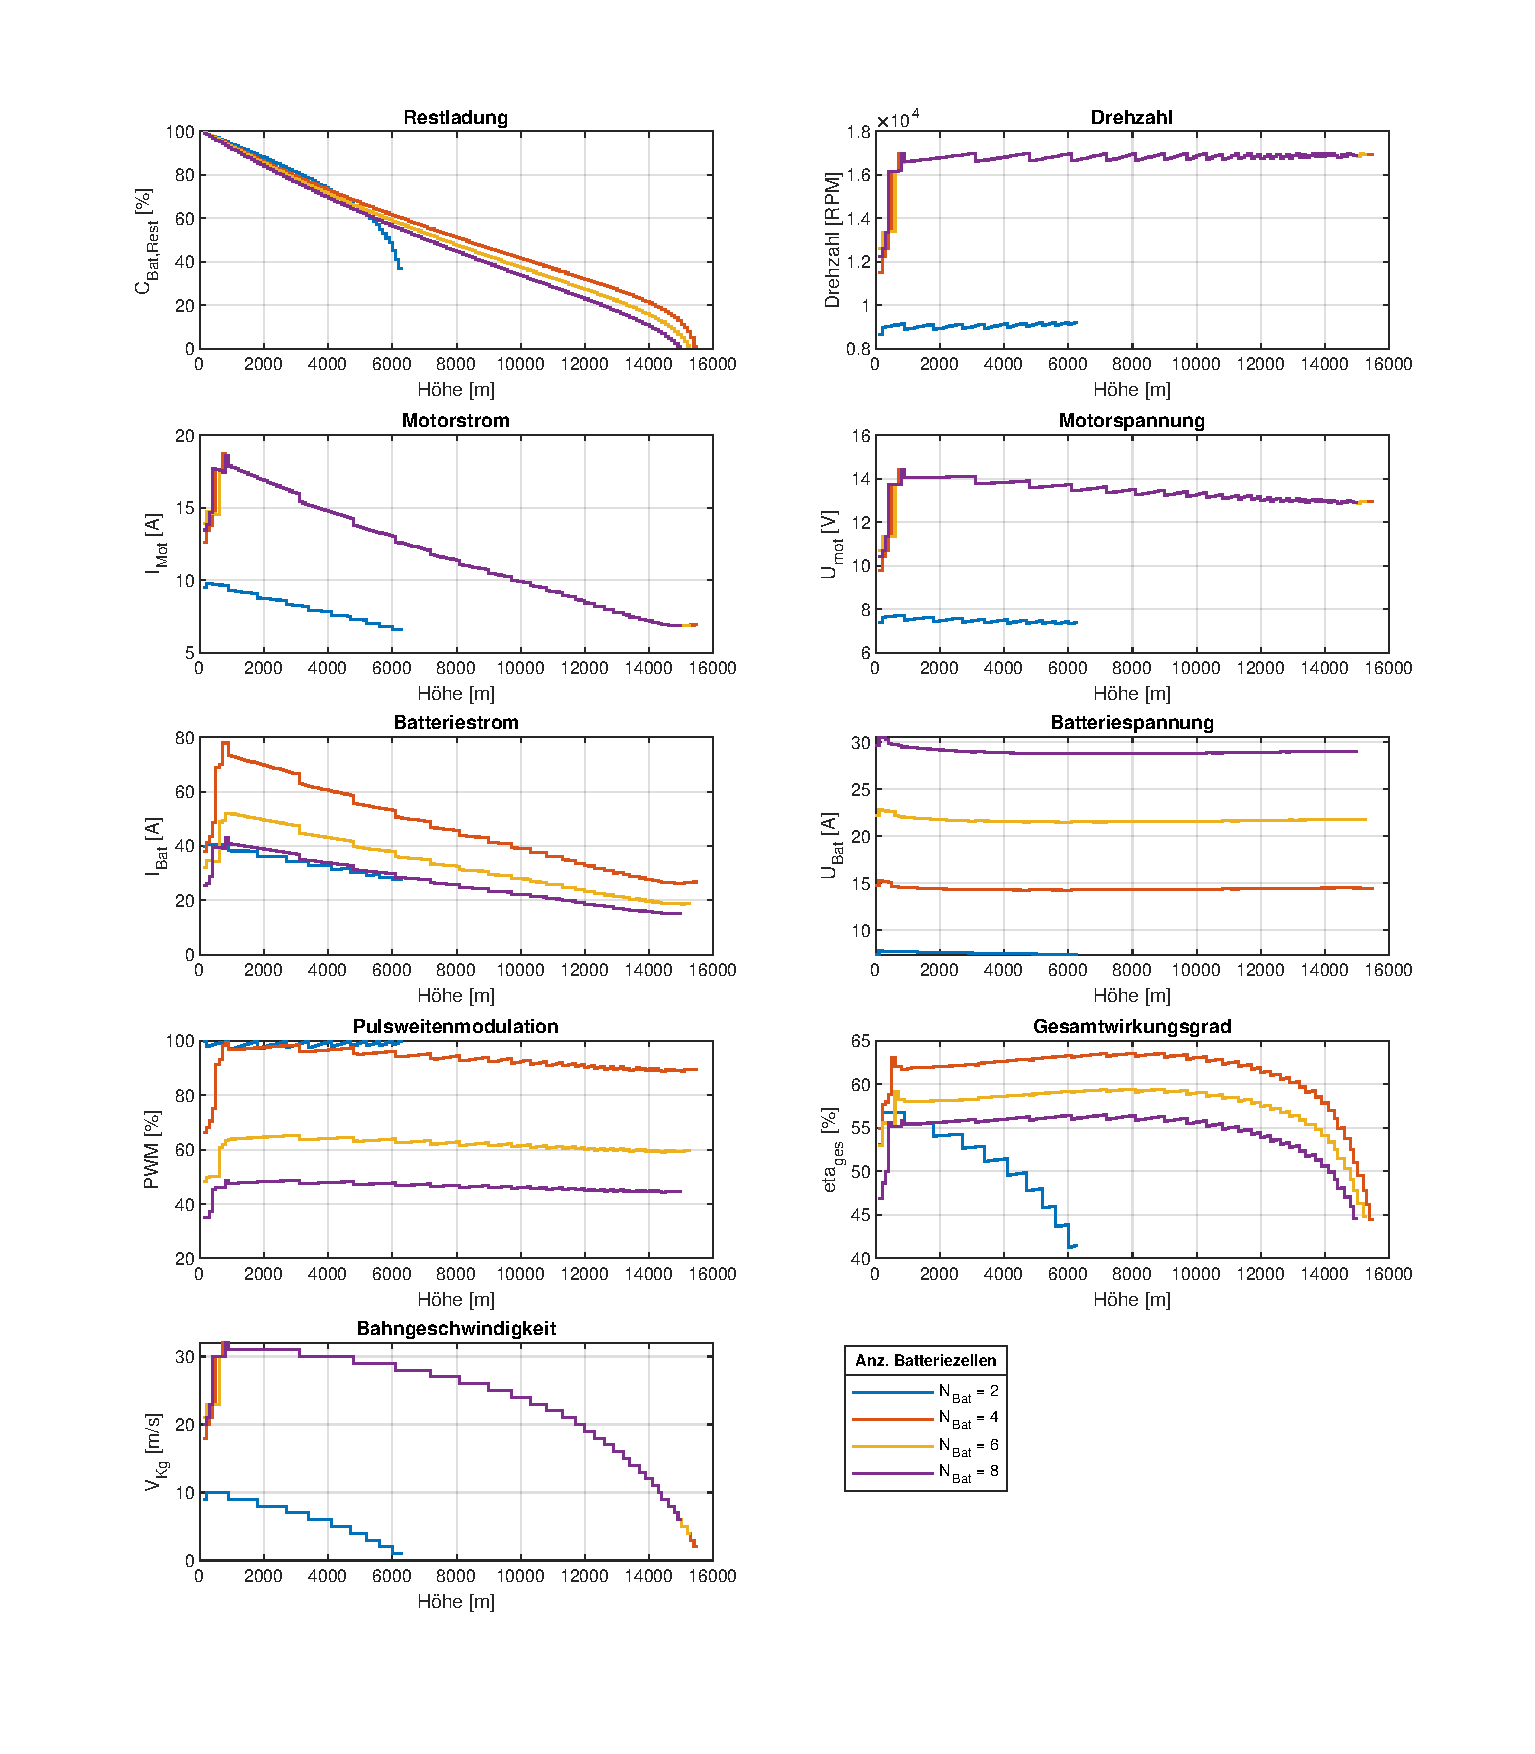
\includegraphics[scale=0.70]{Diagramme/Untersuchung_N_Bat.pdf}
	\caption{Einfluss des Batteriezellenanzahl auf die Flugleistungen der Multicopter-Referenzkonfiguration (Tab. \ref{tab:referenzkonfiguration_mulitcopter})}
	\label{abb:N_Bat_einfluss}
\end{figure}

\subsection{Bedeutung des Motorreglerwirkungsgrades}
\label{subsec:einfluss_eta_pwm}
Der Wirkungsgrad des ESC ist ausschließlich als eine Funktion der PWM modelliert (vgl. Gleichung \ref{eq:eta_pwm}). Wie bereits in Abschn. \ref{subsec:einfluss_n_bat} erklärt, sinkt die PWM mit der Erhöhung der Batteriezellenanzahl. Zeitgleich steigen die Verluste im Motorregler. Im Sinne eines besseren Gesamtwirkungsgrades und der erreichbaren Höhe ist eine Verringerung der Reglerverluste anzustreben. Die Ergebnisse sind in \ref{sec:motorreglerwirkungsgrad} dargelegt. \\
Der Motorreglerwirkungsgrad hat keinen Einfluss auf die Dienstgipfelhöhe. Es ist allerdings ein bedeutender Einfluss auf die Restladung zu erkennen. Mit einem höheren ESC-Wirtkungsgrad steigt auch der Gesamtwirkungsgrad. Weiterhin sinkt der Batteriestrom (vgl. Gleichung \ref{eq:batteriestrom}) mit dem Reglerwirkungsgrad und über den geringeren Batteriestrom sinkt die der Batterie entnommene Kapazität. Werden die Kurven der Restladung linear extrapoliert, so würde die Konfiguration mit sechs Zellen und bei einer Halbierung der Verluste im Motorregler ohne die Dienstgipfelhöhe bereits \SI{18000}{m} und mit keinen Verlusten im Regler bereits mehr als \SI{20000}{m} Höhe erreichen. \\
Daher sind aus den oben genannten Gründen die Verluste innerhalb des Reglers zu verringern. 


\subsection{Einfluss des maximalen Motorstroms}
Die Ergebnisse zeigen, dass ein geringer maximaler Motorstrom ebenfalls die Steiggeschwindigkeit begrenzt. Dieser begrenzt die dem Motor entnommene Leistung. 
Folglich ist ein Motor für einen solchen Steigflug zu wählen, der einerseits einen hohen \ensuremath{K_V}-Wert besitzt, andererseits aber auch einen hohen maximalen Dauerstrom besitzt (vgl. Kap. \ref{subsec:anz_mot_flaechenflzg}). Ein gutes Beispiel ist der Motor aus Kapitel \ref{subsec:mot_prop_kombi} mit einem \ensuremath{K_V}-Wert von \SI{1390}{RPM/V} und einem maximalen Motorstrom \ensuremath{I_{max}} von \SI{35}{A}.



%******************************************************************

\section{Massenanteile der Komponenten}
\label{sec:massenverteilung}
Ein weiterer wichtiger Punkt, der an dieser Stelle untersucht werden soll, ist die Massenanteilsverteilung von den Motoren, der Batterie und der Leermasse des Multicopters am Gesamtgewicht. Wiederum stellt der Quadrocopter aus Kapitel \ref{sec:komponenten} die Grundlage der Untersuchung dar. Bei diesem nehmen die Motoren \SI{13,77}{\%}, die Batterie \SI{52,83}{\%} und die der Rahmen mit den übrigen Komponenten \SI{33,4}{\%} der Gesamtmasse von \SI{1060}{g} ein. Für einen Gegenvergleich wird nun ein anderen Quadrocopter mit diesen Massenverhältnissen erstellt. Als Anhaltspunkt dient die Masse der Motoren, da diese durch die Datenbank vollständig definiert sind. Alle anderen Massenverteilungen ergeben sich im Anschluss aus der Motormasse.
\todo[inline]{bleibt das hier so?}
Die Massen errechnen sich nach folgendem Schema:
\begin{align}
	m_{ges} &= \frac{n_{Prop}\cdot m_{Mot}}{0.1377} , \\
	m_{Bat} &= m_{ges}\cdot 0.5283 , \\
	m_{copter} &= m_{ges}\cdot 0.334.
\end{align}
Zusätzlich wird jeweils auch die obere Stirnfläche \ensuremath{F_{copter,oben}} mit der Größe angepasst. 

\begin{figure}[H]
\centering
	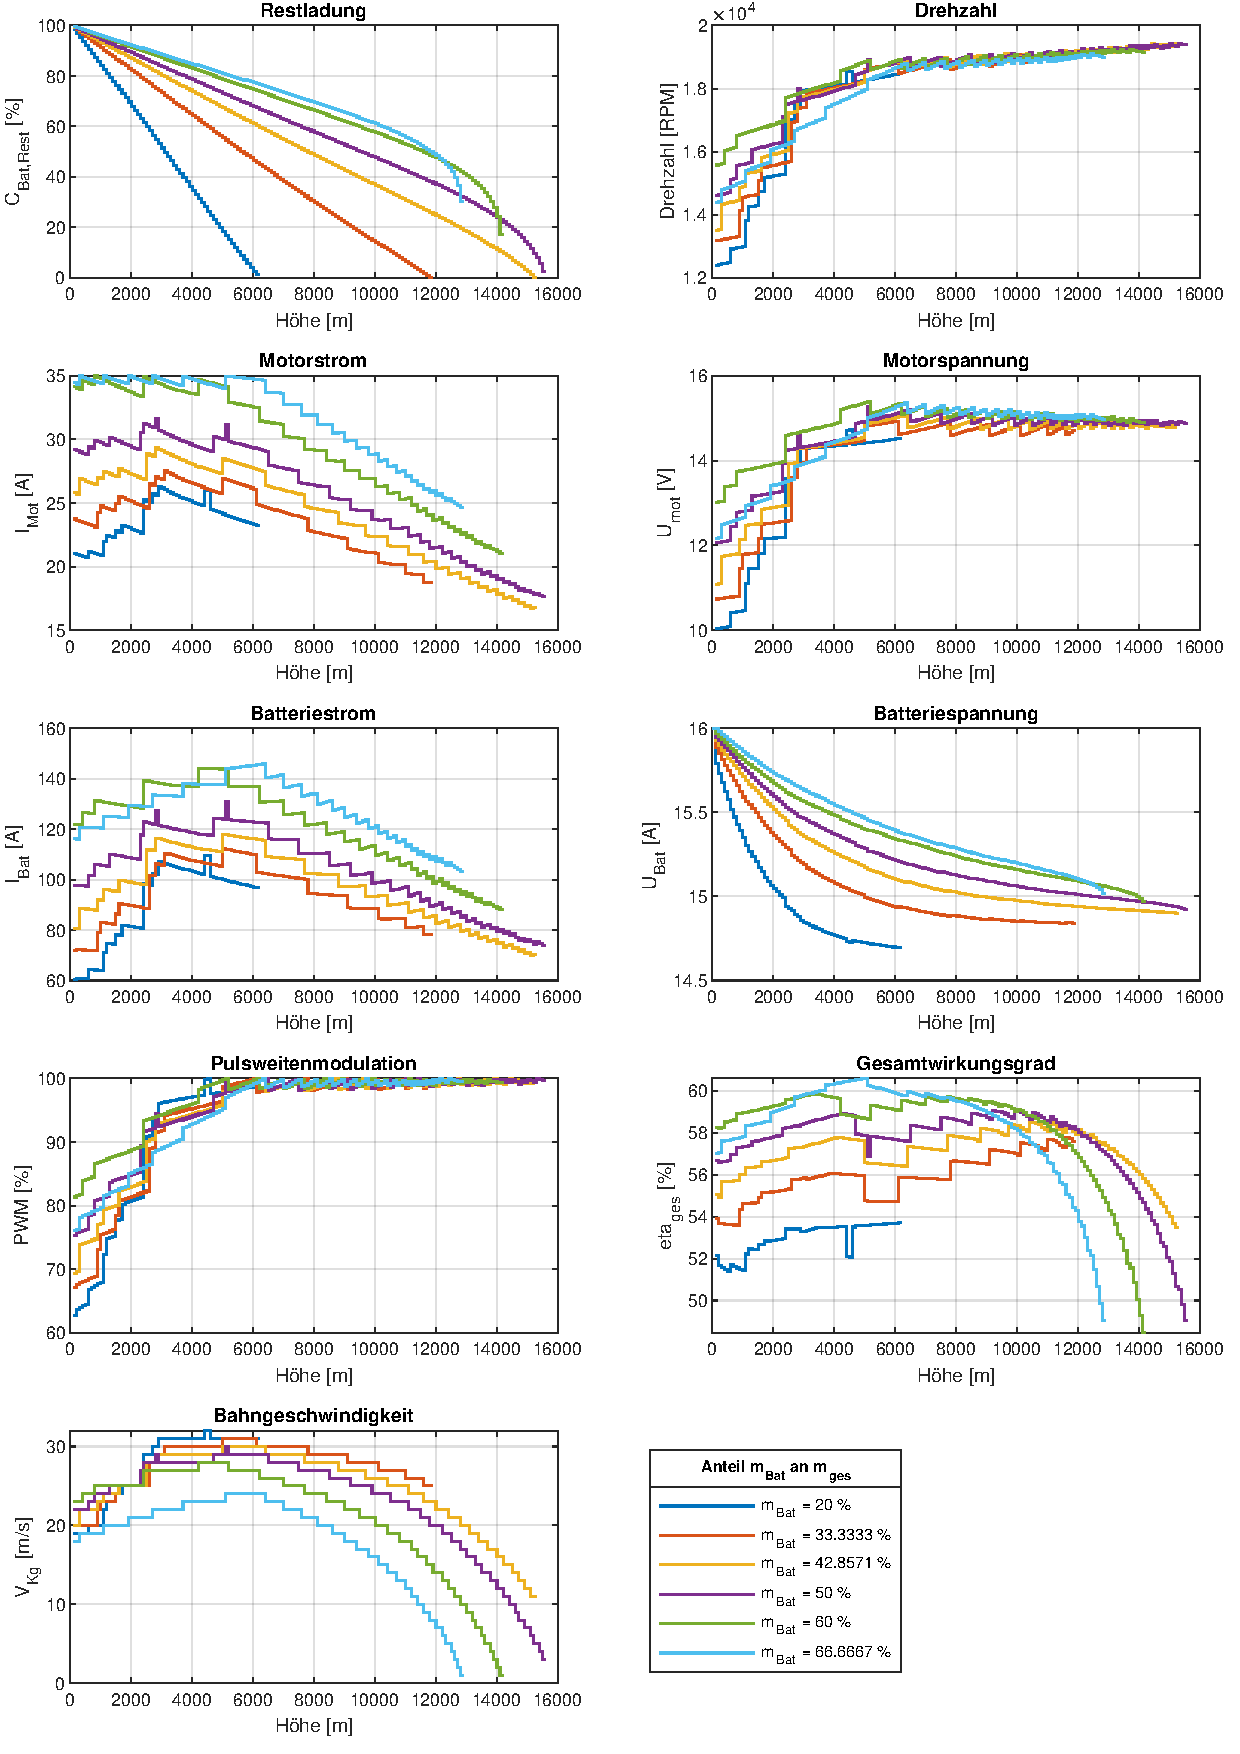
\includegraphics[scale=0.70]{Diagramme/Batteriemasse.pdf}
	\caption{Einfluss des Batteriemassenanteils auf die Flugleistungen der Multicopter-Referenzkonfiguration (Tab. \ref{tab:referenzkonfiguration_mulitcopter})}
	\label{abb:batteriemasse}
\end{figure}

Der Einfluss der Batteriemasse auf die Flugleistungen ist bedeutend (vgl. Abb. \ref{abb:batteriemasse}). Die TOCs variieren in eine Spanne von \SI{5000}{m}. Hier kommt es zu einer Überlagerung zweier Effekte. Der erste ist der Einfluss der Batteriezellenanzahl, der bereits in Abschn. \ref{subsec:einfluss_n_bat} genauer erklärt wurde, und der zweite ist der Einfluss der Batteriemasse. \\
Es kann festgehalten werden, dass mit der Batteriemasse die Batteriekapazität steigt (vgl. Gleichung \eqref{eq:batteriekapazitaet}). Die zur Verfügung stehende Energie erhöht sich. Außerdem erhöht eine höhere Batteriemasse die Gesamtmasse (vgl. Gleichung \eqref{eq:masse_multicopter}) und als Konsequenz auch den erforderlichen Propellerschub (vgl. Gleichung \ref{eq:neigungswinkel} und \ref{eq:schub_multicopter}). Diesem folgt eine Erhöhung des Motor- (vgl. Gleichung \ref{eq:motorstrom}) und des Batteriestroms (vgl. \ref{eq:batteriestrom}).
Bei Batteriemassenanteilen von weniger als \SI{33,33}{\%}, also einem Drittel der Gesamtmasse, limitiert die Batteriekapazität den Steigflug. Durch die geringe Masse werden die Motoren nicht vollständig ausgelastet, sodass der Motorstrom mit dem Drehmoment des Propellers kontinuierlich ansteigt (vgl. Gleichung \ref{eq:motorstrom}). Der Drehzahlzuwachs ist zudem signifikant größer als bei höheren Batteriemassenanteilen. Entsprechend steigt auch die Motorspannung an (vgl. Gleichung \ref{eq:motorspannung}). Der Batteriestrom steigt äquivalent zum Motorstrom und -spannung (vgl. Gleichung \ref{eq:batteriestrom}).
Zudem ist ein stärkerer Spannungseinbruch zu verzeichnen, je kleiner der Batteriemassenanteil ist. Eine Erklärung liefert die Entladerate, die sich aus dem Batteriestrom in Abhängigkeit der Kapazität zusammensetzt und für eine geringere Kapazität steigt (vgl. Gleichung \ref{eq:c_rate}). Die Bahngeschwindigkeit ist jedoch am höchsten und sinkt mit höherem Gesamtgewicht, weil der Schub und letztlich die notwendige Energie mit dem Gewicht und der Bahngeschwindigkeit steigen. 
Weiterhin kann die Dienstgipfelhöhe durch die Motorleistung nicht erreicht werden. Bei sehr kleinen Batterien reicht hierzu die Kapazität nicht aus. Deshalb kann der volle Leistungsüberschuss nicht genutzt werden. 
Anders ist dies, wenn die Batterie die Hälfte der Gesamtmasse ausmacht. Auch hier limitiert die Batteriekapazität die Flughöhe. Jedoch ist die absolute Kapazität bedeutend höher, weshalb auch die maximale Flughöhe höher ist. Wiederum kann der Einfluss der Batteriezellenanzahl auf Batterien mit der gleichen Masse und Kapazität beobachtet werden. Dieser Zusammenhang wird in Abschn. \ref{subsec:einfluss_n_bat} genauer beschrieben. Ab dieser Batteriemasse ist wieder ein effizienter Flug mit maximalen Motorstrom möglich. Je nach der Batteriezellenanzahl ändert sich auch die Dienstgipfelhöhe. Bei \ensuremath{n_{Bat,cell} = 6} ist dies wiederum durch die maximale Propellerdrehzahl begrenzt und bei \ensuremath{n_{Bat,cell} = 4} limitiert die PWM die Motorleistung, sodass der Schubüberschuss aufgebraucht ist. Die Abhängigkeit der Flugleistungen von der Batteriezellenanzahl zeigt auch die Batterie mit einem Massenanteil von \ensuremath{2/3} an der Gesamtmasse. Hier ist die Batteriekapazität wieder größer. Dies verdeutlicht sich in der nochmals geringeren Batteriekapazitätsabnahme. Mit der Masse sinkt auch die Propellerdrehzahl. Durch die größere Gesamtmasse steigt der benötigte Standschub (vgl. Gleichung \ref{eq:neigungswinkel} und \ref{eq:schub_multicopzer}) und damit sinkt die optimale Bahngeschwindigkeit.
%, weil die Bahngeschwindigkeit mit dem Widerstand erhöht (vgl. Gleichung \ref{eq:widerstand}).
Zum Schluss steigert der Batteriemassenanteil noch den Geamtwirkungsgrad. 
Ein Optimum des Batteriemassenanteils liegt bei \SI{66,667}{\%} der Gesamtmasse. Dabei ist vor allem noch die Anzahl der Batteriezellen zu berücksichtigen. Im Hinblick auf Abschn. \ref{subsec:einfluss_n_bat} ist die Zellenanzahl auf den Motor anzupassen, sodass die Motorleistung die maximale Höhe nicht begrenzt, wobei der Motorregler verlustarm arbeiten sollte. Auf der anderen Seite sollte die nominelle Batteriespannung nicht so hoch sein, dass die PWM zum Schutz des Motors abgeriegelt werden muss (vgl. Abschn. \ref{subsec:einfluss_n_bat}). 
Der hier ermittelte optimale Batteriemassenanteil stimmt mit den Aussagen von Neitzke überein \cite{Neitzke.2013}.
Es ist außerdem ersichtlich, dass die Flugleistung und -dauer noch weiter verbessert werden können, wenn der Massenanteil des Rahmens und aller übriger Komponenten kleiner wird und die Masse der Batterie im Gegensatz steigt, d.h. eine Tendenz der Multicopterleermasse gegen Null (\ensuremath{m_{Copter}\rightarrow 0} und \ensuremath{m_{Bat}\rightarrow (m_{Bat}+m_{Copter})}).


%******************************************************************

\section{Größe und Anzahl der Propeller des Fluggerätes}
\label{sec:groesse}
\subsubsection{Größe}
\label{subsubsec:groesse}
Ein weitere Einfluss auf die Flugleistungen stellt das Gesamtgewicht des Fluggerätes dar. Dabei wird das Fluggerät äquivalent skaliert. Dies bedeutet, dass die Massenverhältnisse von Motoren, Batterien und die Leermasse im Verhältnis zum Gesamtgewicht konstant bleiben. Das Verhältnis orientiert sich an der Massenverteilung aus Kapitel \ref{sec:massenverteilung}. Dieses Verhältnis wird für jede Größenskalierung gewahrt. Als Anhaltspunkt dient wieder die Motormasse. Die Propellerauswahl findet nach den Herstellerempfehlungen und eigenen Versuchen statt. Alle anderen Massenverteilungen ergeben sich im Anschluss aus der Motormasse analog zu Kapitel \ref{sec:massenverteilung}.

\begin{figure}[H]
%\centering
	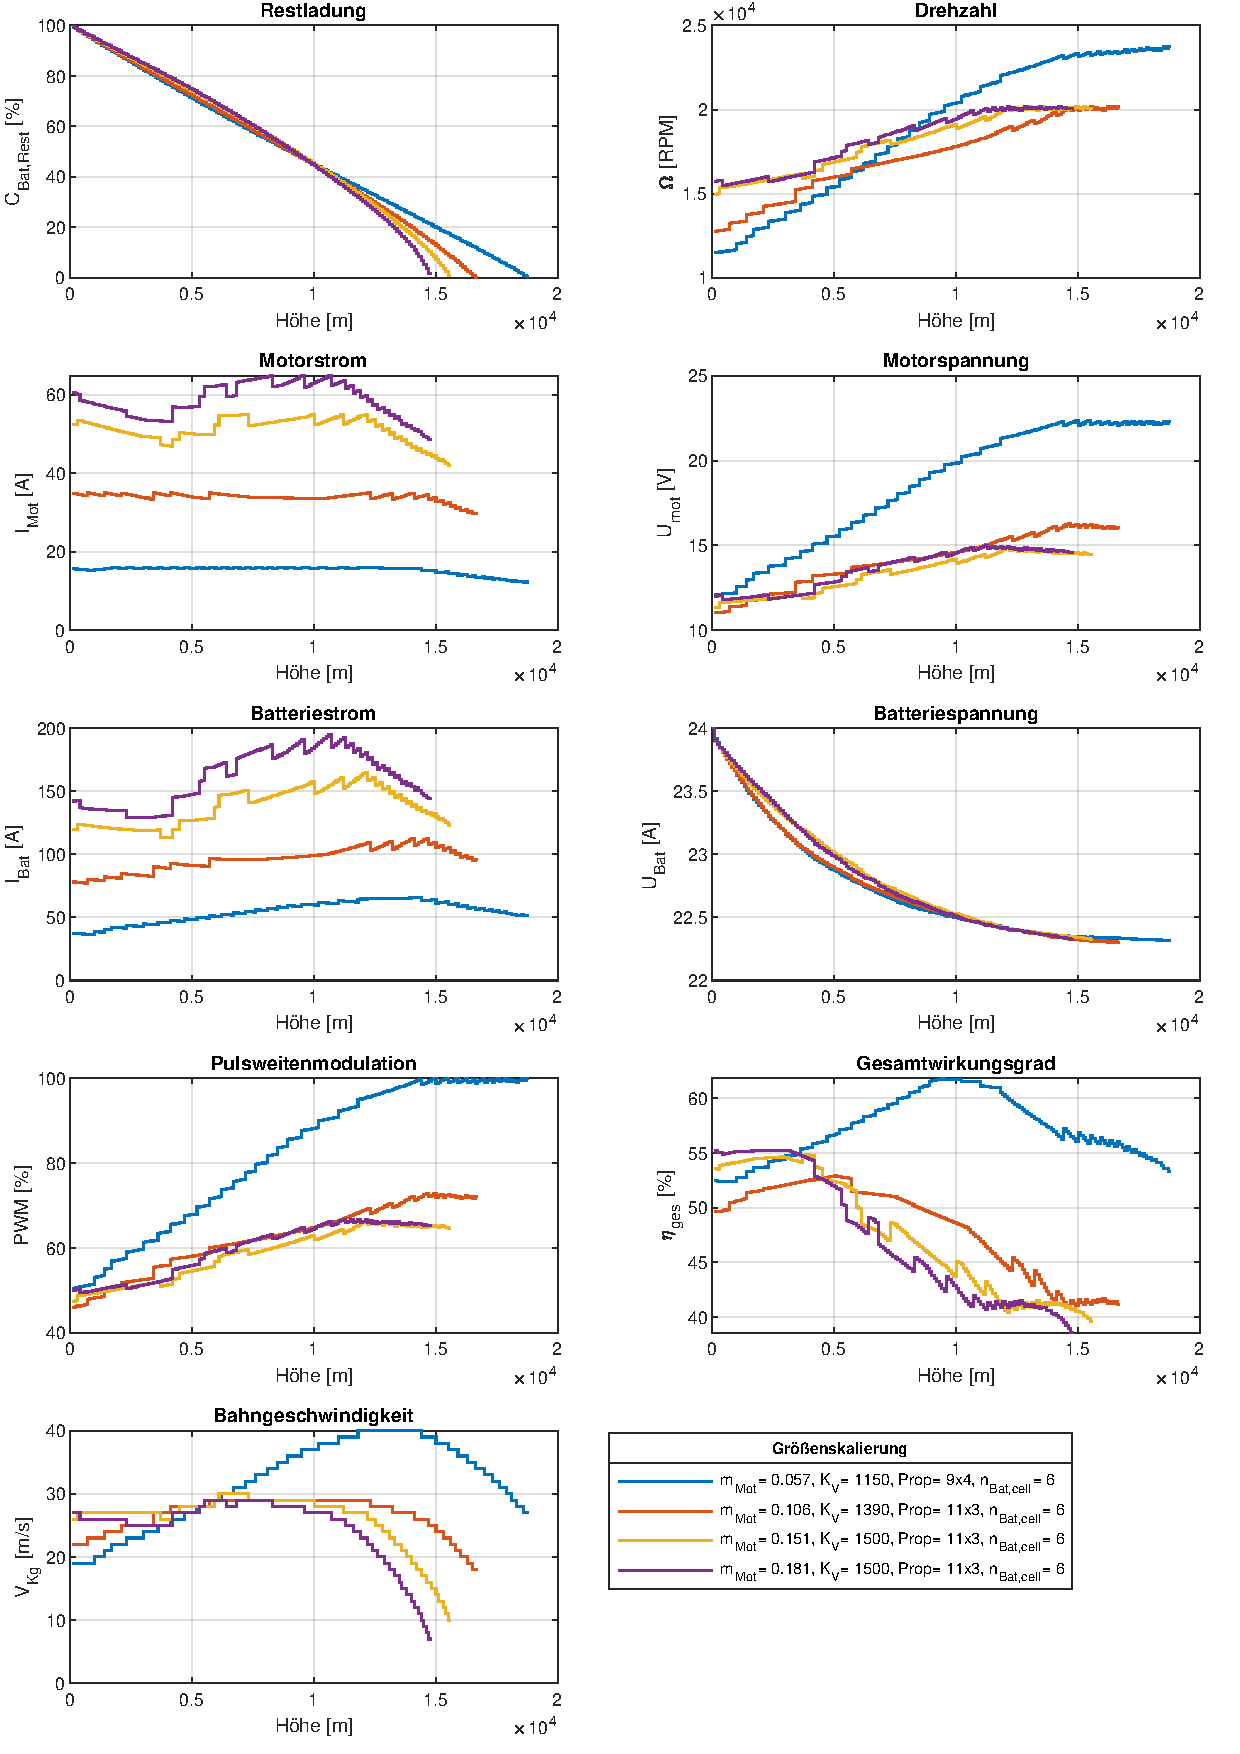
\includegraphics[scale=0.7]{Diagramme/Groessenskalierung.pdf}
	\caption{Einfluss der äquivalenten Größenveränderung auf die Flugleistungen der Multicopter-Referenzkonfiguration (Tab. \ref{tab:referenzkonfiguration_mulitcopter})}
	\label{abb:groessenskalierung}
\end{figure}
Eine äquivalente Größenskalierung besitzt einen vernachlässigbar kleinen Einfluss auf die Flugleistungen (vgl. Abb. \ref{abb:groessenskalierung}). Die Abnahme der Restladung ist für alle Konstellationen beinahe identisch. Der Grund für die Unterschiede in den Diagrammen, die vor allem die Höhe betreffen, liegt in den Unterschieden der Motoren und Propeller. Eine hundertprozentig uniforme Skalierung ist hier nicht möglich. Dabei unterscheiden sich besonders die \ensuremath{K_V}-Werte der Motoren. Dies zieht Unterschiede im Bereich der Motorspannung und folglich in der PWM und im Gesamtwirkungsgrad nach sich. \\
An dieser Stelle kann somit festgehalten werden, dass eine Größenskalierung keinen Einfluss auf die Flugleistungen hat. Die Vorteile einer größeren Masse liegen für reale Anwendungsfälle vorrangig in der Massenträgheit. In einem Höhensektor von \SI{0}{m} bis \SI{15000}{m} treten im Durchschnitt \SI{100}{km/h} starke Winde auf \cite{Seidel.2011}. Die Einflüsse von Böen in diesen Größenordnungen auf einen Multicopter fallen geringer aus, wenn das Fluggerätes auf eine höhere Gesamtmasse ausgelegt wird. Dies erfordert im Umkehrschluss weniger Energie zur Kurs- und Lagekorrektur. \\
Im Hinblick auf die angedachte Nutzlast von \SI{250}{g} im Rahmen des AEROMET\_UAV-Projektes bietet eine größere Gesamtmasse den Vorteil, dass die feste Masse der Nutzlast anteilig an der Gesamtmasse weniger wird, je größer die Gesamtmasse ist.


\subsubsection{Anzahl der Propeller}
\label{subsubsec:anz_prop}
% Wie sich in Abschn. \ref{subsubsec:groesse} zeigte, hat eine uniforme Skalierung des Fluggerätes keinen Einfluss auf dessen Flugleistung. 
Bisher wurden dabei nur Fluggeräte mit vier Rotoren untersucht. Dabei gilt es noch die Abhängigkeit der Flugleistungen von der Propelleranzahl zu überprüfen. 

\begin{figure}[H]
%\centering
	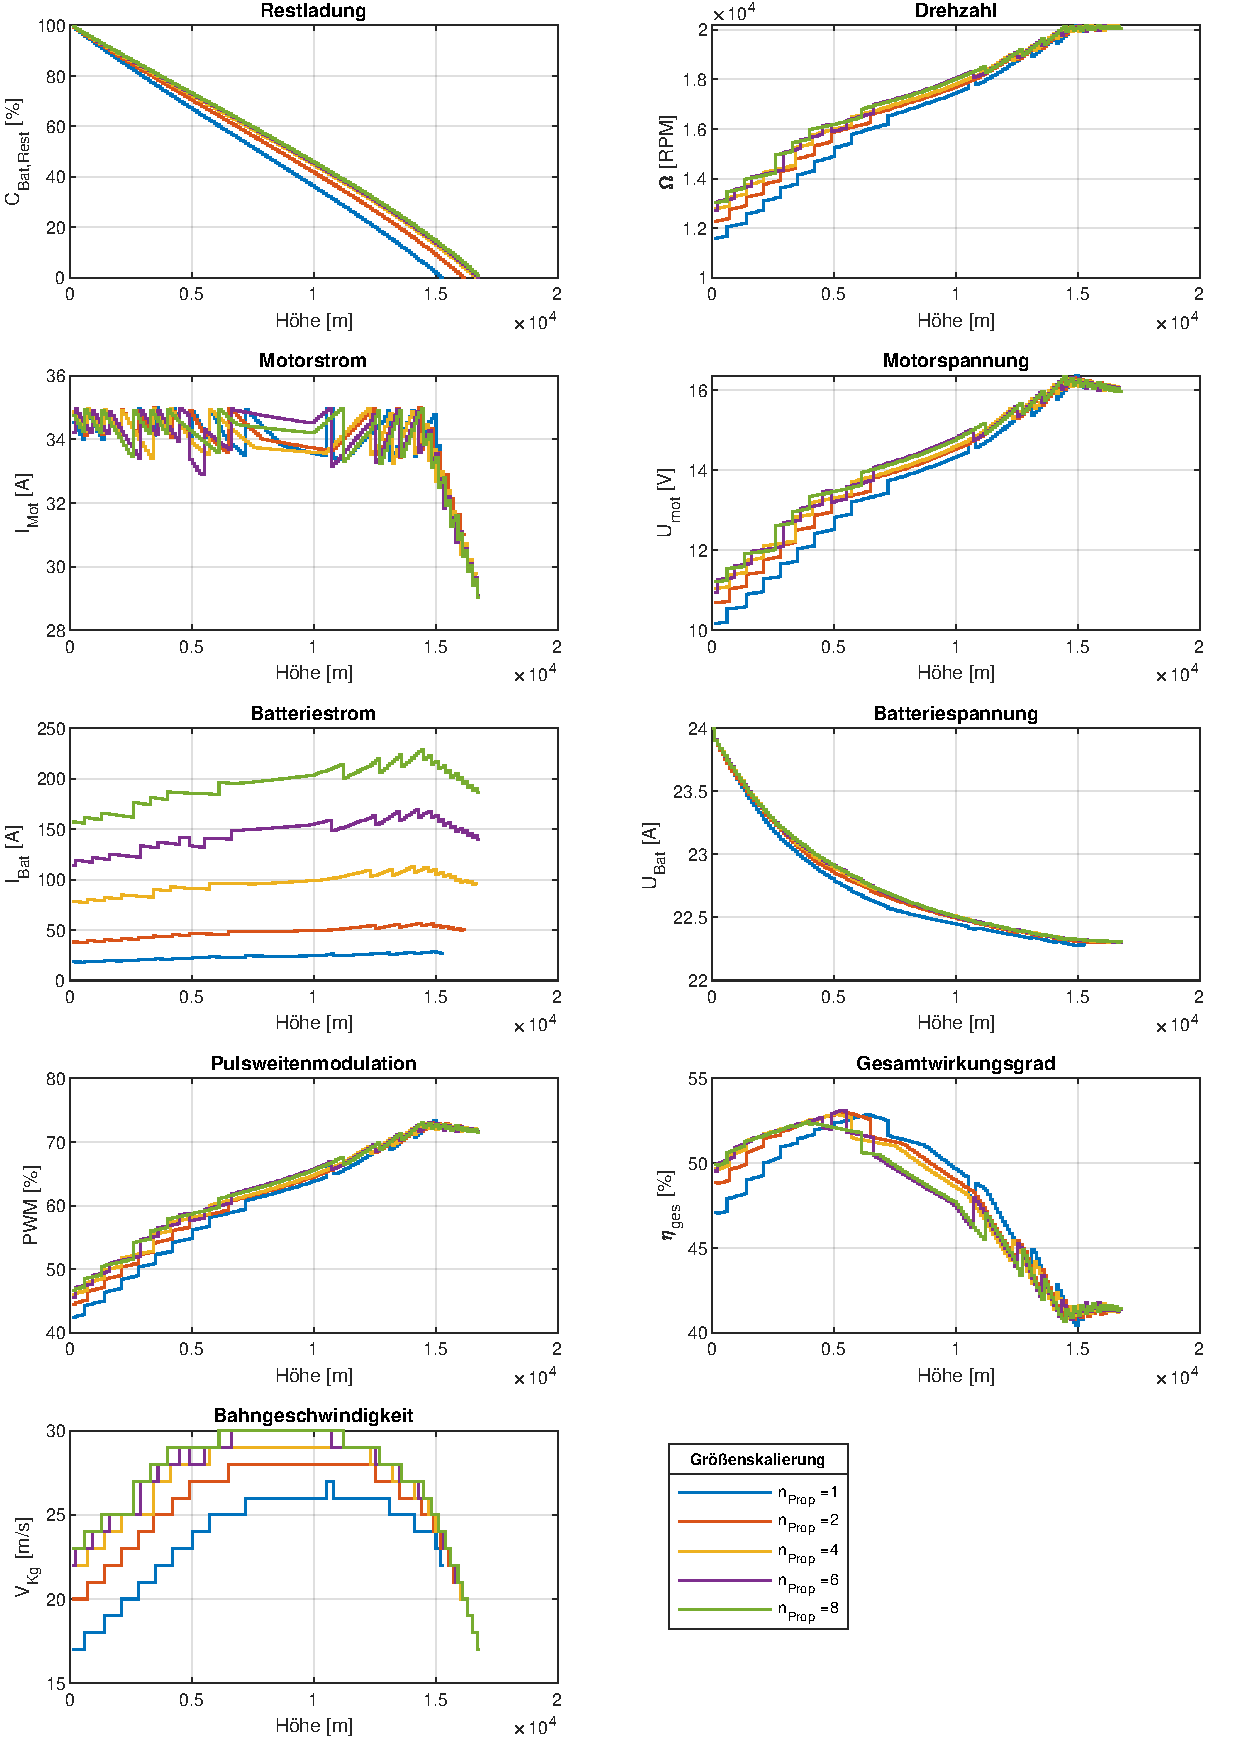
\includegraphics[scale=0.7]{Diagramme/Anz_Prop.pdf}
	\caption{Einfluss der Propelleranzahl auf die Flugleistungen der Multicopter-Referenzkonfiguration (Tab. \ref{tab:referenzkonfiguration_mulitcopter})}
	\label{abb:groessenskalierung}
\end{figure}
Analog zu den Ergebnissen aus Abschn. \ref{subsubsec:groesse} bewirkt eine äquivalente Veränderung der Rotoranzahl keine nennenswerten Änderungen der maximalen Flughöhe, wenn die verwendeten Motoren dieselben sind. Die Ergebnisse für einen Multicopter mit vier, sechs oder acht Propellern sind nahezu identisch. Dies gilt auch für die Restladung, die für diese Konfigurationen im Vergleich zu den Konfigurationen mit weniger Propellern noch pro Höhenschritt mehr Restladung aufweisen. Die einzigen Unterschiede weisen der Batteriestrom und die Bahngeschwindigkeit auf. Der Batteriestrom erhöht sich mit beinahe konstanten \SI{50}{A} pro zusätzlichen zwei Propellern (vgl. Gleichung \ref{eq:batteriestrom}). Dahingegen steigt auch die Bahngeschwindigkeit mit mehr Propellern. \\
An dieser Stelle sind jedoch Einschränkungen vorzunehmen. 
Der Monocopter erreicht ähnliche Flugleistungen wie die anderen Konfigurationen. Der Monocopter benötigt jedoch zusätzlich noch Aktuatorik für die Abdeckung der restlichen drei Stellgrößen. Das umfasst Aktuatorik für das Nicken, Rollen und Gieren. Die translatorische Fortbewegung kann bereits durch den Propeller erfolgen. Der Drehmomentenausgleich könnte durch eine der drei rotatorischen Stellgrößen erfolgen (z.B. Rollen). Insgesamt sind also mindestens drei weitere Aktuatoren notwendig. Diese zusätzliche Aktuatorik benötigt der Duocopter ebenfalls. Ein Drehmomentenausgleich ist hier jedoch nicht notwendig. Trotzdem werden hier immerhin noch zwei weitere Aktuatoren für das Nicken und Gieren benötigt. 
Beide erwähnten Punkte erhöhen die Gesamtmasse und benötigen zusätzlich Energie. Dies verringert die Gesamthöhe. 
Für mehr als vier Propeller muss berücksichtigt werden, dass die Gesamtmasse und damit insbesondere das Strukturgewicht steigt. Dies geht auf die Kosten einer optimalen Konstellation der Massenverteilung. Zusätzlich erhöht sich die obere Stirnfläche \ensuremath{F_{copter,oben}} durch stärkere Strukturen, die in einer Widerstandserhöhung und somit erhöhten Verlusten resultieren. 
Für den anschließenden Sinkflug wäre ein um die Gierachse eigenstabiler und um die Roll- und Nickachse mit den zusätzlichen zwei Aktuatoren steuerbarer Duocopter, welcher die beiden Antriebe abschaltet und sich somit im Gleichtflug befindet, womöglich sehr effizient. Diese Art der Konfiguration spricht für einen Gleitflüger, der die beiden genannten Eigenschaften verbindet.
Um das oben gesagte zusammenzufassen, eignet sich eine Propelleranzahl von mindestens zwei am besten für einen Flug in die untere Stratosphäre. \\


\section{Verstellpropeller}
\label{sec:verstellprop}
Eine bisherige Begrenzung der Flugleistungen erfolgte häufig durch die maximale Drehzahl des Propellers, die indirekt die Motorspannung beeinflusst. 
Besonders auffällig bei vorherigen Untersuchungen (vor allem in Bezug auf die Untersuchungen des Quadrocopters aus Kap. \ref{chap:nachbildung_des_quadrocopter}) ist, dass die Drehzahl von Propellern mit einer geringen Steigung deutlich schneller steigt als bei einem Propeller mit einer großen Steigung. Da vor allem die Drehzahl die Motorspannung bestimmt, ist eine Verringerung der Drehzahl bei gleichem Schub von Interesse. Mit zunehmender Flughöhe verringert sich die Dichte und dementsprechend auch der Schub, wenn die Rotordrehzahl und die Propellersteigung konstant gehalten werden. Diesem Effekt kann mit einer Erhöhung der Drehzahl oder mit einer Erhöhung der Steigung entgegen gewirkt werden. Während bei einem Drehflügler mit Strahltriebwerk nur eine Blattverstellung, nicht aber eine Drehzahlerveränderung möglich ist, besitzen elektrisch, propellergetriebene Fluggeräte beide Möglichkeiten. Dies kann mit einem Verstellpropeller und entsprechender Aktuatorik realisiert werden. \\
Im Rahmen dieser Untersuchung liegen nur Propellerkennfelder mit einer konstanten Propellersteigung vor. Das Vorgehen für einen Propeller mit variabler Steigung sieht so aus, dass für einen vorgegebenen Durchmesser alle Kennfelder mit diesem Durchmesser der Datenbank entnommen werden (siehe \ref{sec:vprop_vorgehen}). Danach wird in der Leistungsuntersuchung jeder Propeller mit unterschiedlicher Steigung, aber gleichem Durchmesser, gegeneinander abgewogen. Die Auswahl für den in dem betrachteten Flugmoment beste Steigung erfolgt wieder über die Energiebetrachtung, analog zum Bahnneigungswinkel und der Bahngeschwindigkeit (vgl. Kap. \ref{subsubsec:schub_flaechenflzg}). Dies ist ein Idealfall, weil mit der minimal aufgebrachten Energie auch die der Batterie entzogenen Restladung minimal ist. Folglich wird nur der Zustand ausgewählt, der die größte Restladung aufweist.

\begin{figure}[H]
\centering
	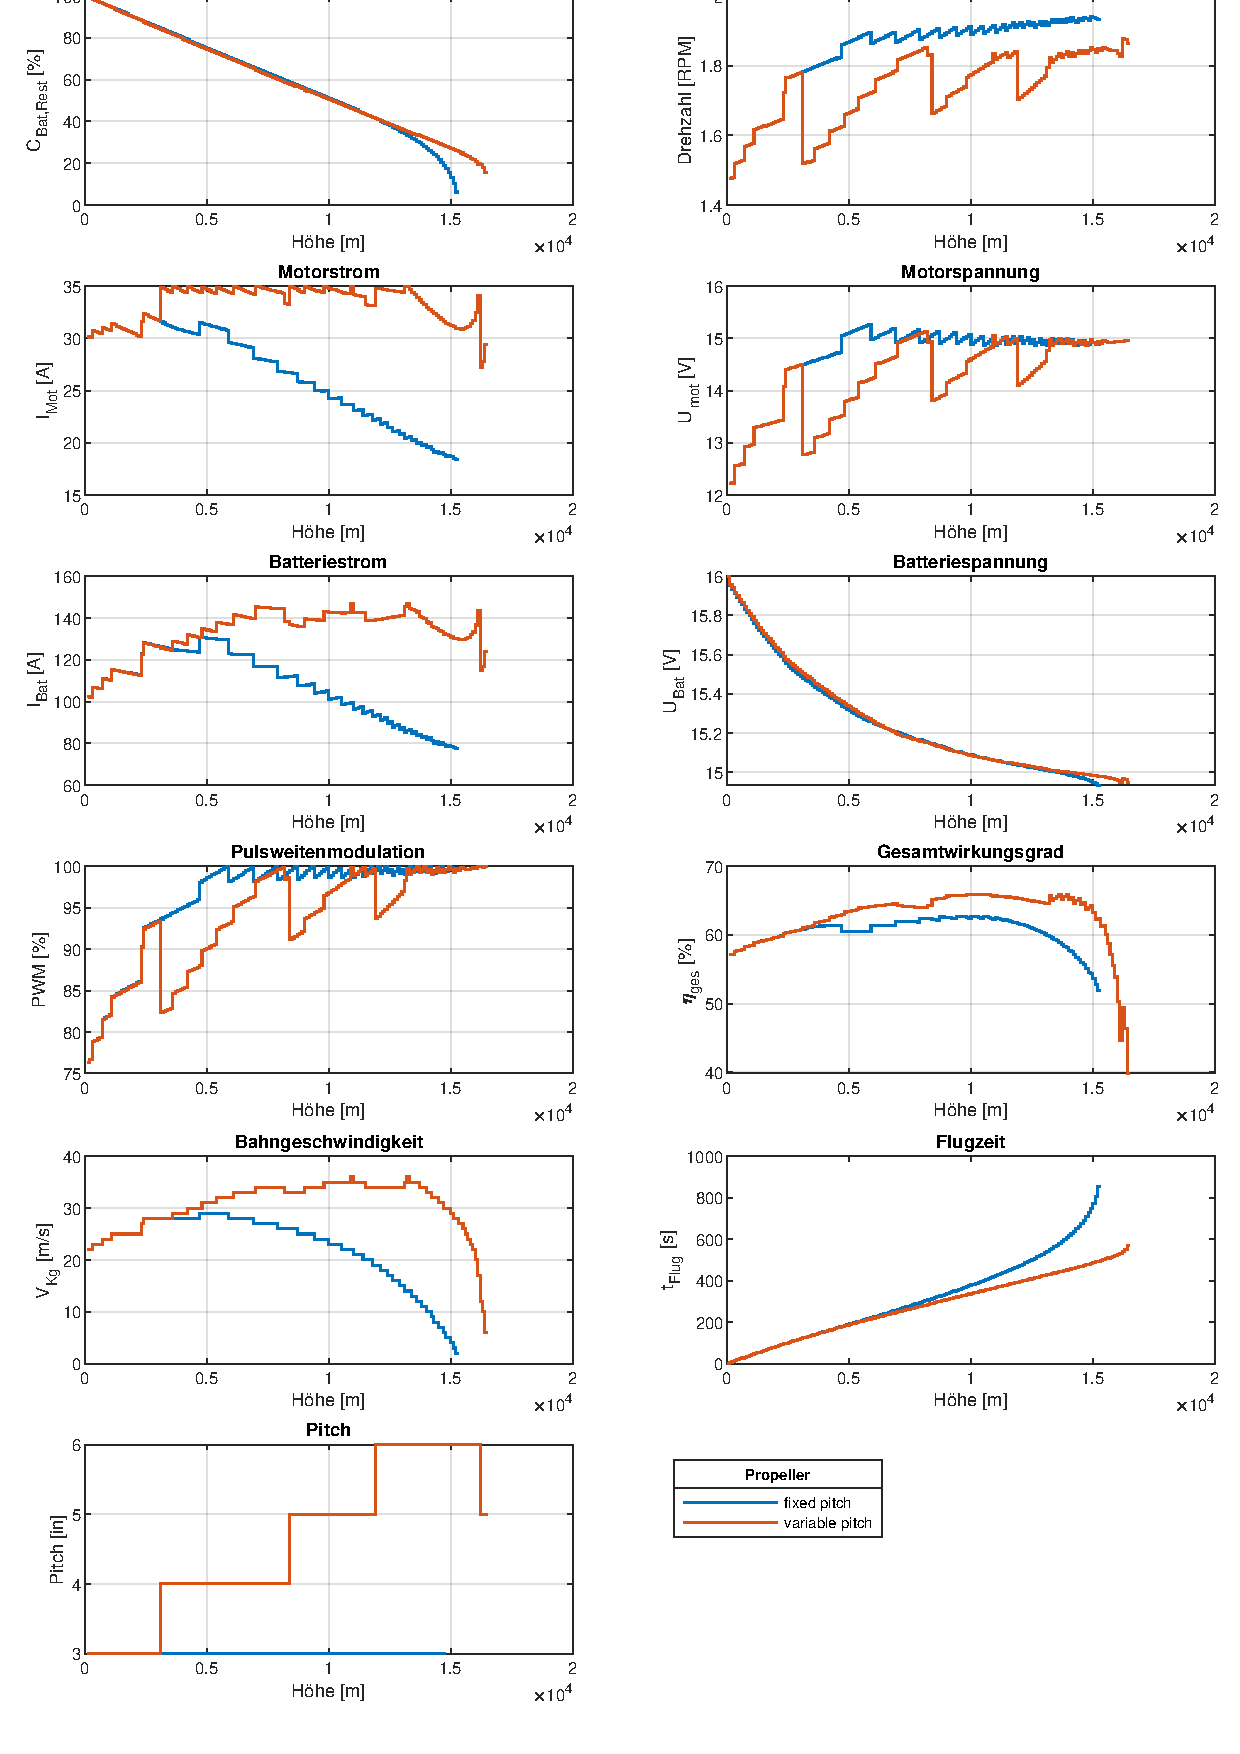
\includegraphics[scale=0.7]{Diagramme/Verstellpropeller.pdf}
	\caption{Einfluss eines idealen (Eigengewicht gleich null und ideale Verwindung) Verstellpropellers auf die Multicopter-Referenzkonfiguration (Tab. \ref{tab:referenzkonfiguration_mulitcopter})}
	\label{abb:verstellpropeller}
\end{figure}
Mit dem Verstellpropeller ist ein deutlicher Höhengewinn von \SI{2000}{m} zu verzeichnen. Selbst mit dem Verstellpropeller wird ab \SI{17500}{m} die Dienstgipfelhöhe erreicht, die sich wieder durch die Begrenzung der Propellerdrehzahl auszeichnet. Ab \SI{17000}{m} ist die Blattspitzengeschwindigkeit  \ensuremath{Ma = 1}. Allerdings sind die Auswirkungen auf die Flugleistungen marginal. Hieraus kann geschlossen werden, dass ein Verstellpropeller die Dienstgipfelhöhe in größere Höhen verschieben kann. \\
Mit dem Verstellpropeller kann durchgehend am effizientesten bei maximalen Motorstrom (hier \ensuremath{I_{max} = \SI{35}{A}}) geflogen werden. Die Propellersteigung wächst im Laufe des Steigfluges von anfänglichen \SI{3}{in} auf \SI{5}{in}. Dies ist erstaunlich, da noch viel größere Steigungen möglich wären, die aber selbst in großen Flughöhen immer noch mehr Energie der Batterie entziehen als kleinere Steigungen. Es gilt also, dass geringe Propellersteigungen für Multicopter am effizientesten mit Hinblick auf den Energieverbrauch sind. Die Fluggeschwindigkeit ist allerdings auch gering, sodass sich hohe Steigungen tendenziell erst bei hohen Fluggeschwindigkeiten lohnen. \\
Signifikant ist der Einfluss einer Propellersteigungsänderung auf die Propellerdrehzahl. Aufgrund der Tatsache, dass der Verstellpropeller mit Kennfeldern von Propellern modelliert wird, die eine feste Steigung besitzen, bedeutet eine Änderung der Propellersteigung auch eine Änderung der Drehzahl. Diese Drehzahleinbrüche treten auf, da ein Propeller mit einer höheren Steigung denselben Schub bei einer geringeren Drehzahl erzeugen kann. Der Verlauf der Drehzahl wirkt sich direkt auf die Motorspannung aus (vgl. Gleichung \ref{eq:motorspannung}), damit auch auf die PWM (vgl. Gleichung \ref{eq:pwm}) und letztlich auf den Batteriestrom (vgl. Gleichung \ref{eq:batteriestrom}). Im Vergleich zum Propeller mit konstanter Steigung ist die PWM durch die vergleichsweise geringere Drehzahl und die geringere Drehzahl unterhalb der PWM der Referenzkonfiguration. Folglich fällt auch der Motorreglerwirkungsgrad schlechter aus. Allerdings wird durch die Propellersteigungsänderung eine deutliche Erhöhung des Propellerwirkungsgrades erzielt. Dies kann auf die langsamer drehenden Propeller, aber deutlich schneller fliegenden Multicopter zurückgeführt werden (vgl. Gleichung \ref{eq:eta_prop}). Eine Propellersteigungserhöhung liefert gleichzeitig auch mehr Schub. Somit ist auch eine höhere Bahngeschwindigkeit möglich. Insgesamt liegt somit der Gesamtwirkungsgrad \ensuremath{\eta_{ges}} vom Multicopter mit Verstellpropeller ab \SI{7000}{m}, wenn die Propellersteigung das erste Mal erhöht wird, ca. \SI{3}{\%} mit einer steigenden Tendenz über dem Multicopter ohne. In \SI{15000}{m} Höhe sind es sogar mehr als \SI{10}{\%}. \\
Eine Änderung auf die Abnahme der Restladung macht sich erst ab ca. \SI{10000}{m} Höhe bemerkbar. Während die Restladung vom Multicopter ohne Verstellpropeller ab dieser Höhe schneller abnimmt, kann sie durch einen Verstellpropeller verlangsamt werden. Dies bedeutet, dass ein Verstellpropeller die Effizienz in niedrigen Höhen nicht bedeutend beeinflusst. Für Steigflüge in großen Höhen kann er jedoch die Effizienz deutlich anheben.
% Dies gilt jedoch nicht bei Steigflügen in noch größere Höhen, da er dort die Effizienz deutlich anhebt.
%Der zusätzliche Höhengewinn durch einen Verstellpropeller liegt bei  ca. \SI{1500}{m} (vgl. Abb \ref{abb:verstellpropeller}). Dabei handelt es sich um einen idealen Verstellpropeller, dessen Verstellmechanismus und -aktuatorik nicht in das Gesamtgewicht einbezogen werden. \\
%Die Leistungsparameter beider Propellerarten sind für die ersten \SI{3000}{m} identisch. Dies liegt an der gleichen Propellersteigung. Danach nimmt die optimale Propellersteigung kontinuierlich zu. Durch die Tatsache, dass die Steigung variabel ist, ist durchgehend ein Flug mit maximaler Motorleistung, d.h. bei einem maximalen Motorstrom und -spannung, möglich. Durch jede Verstellung kommt es zu einem Einbruch der Drehzahl, der sich durch den Verlauf der Motorspannung und der PWM fortpflanzt (entspr. Gleichung \ref{eq:motorspannung} und \ref{eq:pwm}). Bis zu einer Höhe von \SI{3000}{m} hat der Verstellpropeller keinen Einfluss auf die Restladung oder die Batteriespannung. Die deutlich höhere Effizienz des Fluges bei maximalen Motorstrom zeigt sich im Gesamtwirkungsgrad. Durch die mit der Propellersteigungsänderung steigende Bahngeschwindigkeit erhöht sich auch der Propellerwirkungsgrad. Daher erhöht sich auch der Gesamtwirkungsgrad. 
%Ein Vorteil, der in Abb. \ref{abb:verstellpropeller} ersichtlich wird, ist, dass durch eine Erhöhung der Propellersteigung der gleiche, wenn nicht sogar noch mehr Schub, bei einer geringeren Drehzahl durch den Propeller erzeugt werden kann. Dies erhöht den Leistungsüberschuss und letztendlich die erreichbaren Fluggeschwindigkeiten bei voller Motorauslastung. Entsprechend sinkt die Flugzeit.
%Bedeutend ist noch zu erwähnen, dass die Restladung am TOC bei einem Multicopter mit Verstellpropeller noch bedeutend höher ist (insg. noch ca. \SI{20}{\%}) als die bei einem ohne. \\
Der Vorteil eines Verstellpropellers ist deutlich. Dazu müssen aber noch folgende Einschränkungen vorgenommen werden. Der Verstellpropeller kann nur im Rahmen der in der APC-Datenbank \cite{apc} vorhanden Propeller modelliert werden. Dies setzt Ungenauigkeiten voraus, da eine kontinuierliche Verstellung nicht nachgebildet werden kann und nur so viele Verstellungen berücksichtigt werden können, wie auch Propeller mit verschiedenen Steigungen in der Datenbank vorhanden sind. Eine kontinuierliche Verstellung würde an dieser Stelle einen glatten Verlauf in der Propellersteigung und somit auch in allen anderen Verläufen erzeugen. \\
An dieser Stelle wurde der Propeller in gewisser Weise idealisiert. So wurde unter anderem die verlängerte Blattaufhängung mit dem Steuerstangenanschluss und der Verstellaktuatorik etc. außer Acht gelassen. Dies würde zu zusätzlichen Verlusten an der Blattwurzel und einer Verringerung des effektiven Radius führen. Bei einem Propeller mit konstantem Anstellwinkel kann diese sehr kurz gehalten werden, weshalb das profilierte Rotorblatt radial gesehen deutlich früher beginnt. Die Verringerung der effektiven Propellerblattlänge ist bei dem hier modellierten Verstellpropeller nicht berücksichtigt worden. Weiterhin birgt die Verwendung von Propellerkennfeldern mit einer festen Steigung gewisse Ungenauigkeiten. Für die Propeller mit fester Steigung kann vorausgesetzt werden, dass dieser im Rahmen eines optimalen Schwebeflugrotors \cite[S.197-S.205]{Wall.2015} ausgelegt wurde (ausschließlich axiale Anströmung, Betrieb nur im Vorwärtsflug, etc). Ein Verstellpropeller muss jedoch eine gewisse Bandbreite an Betriebspunkten abdecken (Steig-, Vorwärtsflug oder Autorotation), die durch eine einseitige Optimierung des Propellers eine Verschlechterung für die anderen bedeutet \cite[S.203]{Wall.2015}. Es ist daher auch mit Diskrepanzen für das Leistungsverhalten des Verstellpropellers in Bezug auf Propeller mit fester Steigung zu rechnen, die nicht den Kennfeldern zu entnehmen sind. \\
Weiterhin wurden in dieser Betrachtung das Gewicht des Verstellmechanismus an sich und der Aktuatorik für jeden einzelnen Propeller nicht berücksichtigt. Weiterhin bedeuten die Aktuatoren zusätzliche Verbraucher für die Batterie, die mitunter deutlich schneller zu einem Flug bei \SI{100}{\%} PWM führen würden. Letztendlich ist der fehlende Schub in großen Höhen nicht das Begrenzungsmerkmal, sondern die Drehzahl des Propellers und Motors sowie die Batteriespannung, kurz der Leistungsüberschuss. Letzterer macht den Verstellpropeller ein weiteres Stück redundant. %(vgl. \ref{abb:vertellprop_real}). 
Mit einem hohen Batteriestrom verschiebt sich der Bereich, in dem ein größere Steigung vorteilhafter ist, noch weiter in größere Höhen. Damit sinkt auch die Einsatzdauer und schließlich der Nutzen. 
Schlussendlich bringt der Verstellpropeller den Vorteil der Autorotation mit, der weniger für den Steigflug als für den anschließenden Sinkflug von Bedeutung ist. Durch die Autorotation ist ein antriebsloser Sinkflug möglich. Damit könnte die Batterie noch weiter entladen werden bevor ein Sinkflug eingeleitet werden muss, was im Umkehrschluss die erreichbare Höhe steigert. Außerdem erhöht ein Verstellpropeller die Restladung am TOC, sodass das volle Potential dieser Propellerart ausgeschöpft werden kann. Im Zustand der Autorotation ist jedoch kein Ausgleich von Seitenwinden möglich. Die Abdrift muss daher an dieser Stelle negativ bewertet werden. \\
Zusammengefasst gilt, dass ein Verstellpropeller Vorteile in großen Höhen mit sich bringt. Allerdings ist die hier in Abb. \ref{abb:verstellpropeller} dargelegte Effizienz anzuzweifeln. Die Vorteile ergeben sich auch in Abhängigkeit der Konstruktion. Je kleiner die Blattaufhängung ist, desto effizienter ist der Verstellpropeller. Weiterhin ist die Masse des Verstellmechanismus im Verhältnis zum Gesamtgewicht abzuwägen. Je größer das Gesamtgewicht des Multicopters, desto geringer ist der nachteilige Einfluss der Zusatzmasse durch den Verstellpropeller auf dessen Flugleistungen. Aus diesem Grund ist der reale Nutzen für kleinere Multicopter zu verneinen. 
In \ref{sec:vprop_vorgehen} werden die Flugleistungen für einen Verstellpropeller mit Eigengewicht dargelegt. 



\section{Stufenloses Getriebe}
\label{sec:getriebe}
Eine häufige Begrenzung der Leistung ist die maximale Drehzahl des Motors oder des Propellers 
\todo[inline]{hier Verweis einfügen}. Diese nimmt mit großen Höhen stark zu. Ein hypothetisches stufenlos, verstellbares Getriebe bringt den Vorteile mit, dass durch dessen Einsatz die Drehzahl für den Motor entsprechend angepasst werden kann, sodass die Motorspannung nicht mehr den Flaschenhals für einen Steigflug darstellt.
Die Übersetzung für ein Getriebe 
\begin{equation}
	i = \frac{\Omega_{an}}{\Omega_{ab}} 
	\label{eq:getriebe_uebersetzung}
\end{equation}
setzt sich in Abhängigkeit der Drehzahlen aus dem Verhältnis der Eingangsdrehzahl \ensuremath{\Omega_{an}} zur Ausgangsdrehzahl \ensuremath{\Omega_{ab}} zusammen. Weiterhin gilt für die Leistung, dass unter Berücksichtigung von Verlusten innerhalb des Getriebes die Eingangsleistung \ensuremath{P_{an}} gleich der Ausgangsleistung \ensuremath{P_{ab}} ist
\begin{equation}
	P_{an} = \eta_{Getriebe} \cdot \Omega_{an}\cdot M_{an} = \Omega_{ab}\cdot M_{ab} = P_{ab}
	\label{eq:getriebe_leistung}
\end{equation} 
mit dem Getriebewirkungsgrad 
\begin{equation}
	\eta_{Getriebe} = \frac{P_{ab}}{P_{an}} \leq 1 \eqend{.}
	\label{eq:getriebe_wirkungsgrad}
\end{equation}
Aus den Gleichungen \ref{eq:getriebe_uebersetzung} bis \ref{eq:getriebe_wirkungsgrad} ergeben sich nun für die aus dem Propellerkennfeld ermittelten Drehzahl und dem Drehmoment die neue Drehzahl für den Motor
\begin{equation}
	\Omega_{neu} = \Omega_{Kennfeld}\cdot i
\end{equation}
und aus der Leistung
\begin{equation}
	M_{neu} = \frac{P_{ab}}{\Omega_{neu}} \eqend{.}
\end{equation}
das neue Drehmoment.
Die günstigste Übersetzung wird analog zum Steigwinkel des Flächenflugzeuges und analog zur Steiggeschwindigkeit durch eine Iteration über der Übersetzung \ensuremath{i} gefunden (siehe Anhang \ref{sec:getriebe_vorgehen}). Das Entscheidungskriterium ist auch hier die minimal aufgebrachte Energiemenge für den jeweiligen Höhenschritt. An dieser Stelle ist das Getriebegewicht \texttt{m\_Getriebe} nicht zu vernachlässigen. Diese fließt mit der Anzahl der Propeller in die Berechnung der Gesamtmasse mit ein
\begin{equation}
	m = m_{Bat} + (m_{Mot} + m_{Getriebe})\cdot n_{Prop} + m_{Copter} .
\end{equation}

\begin{figure}[H]
\centering
	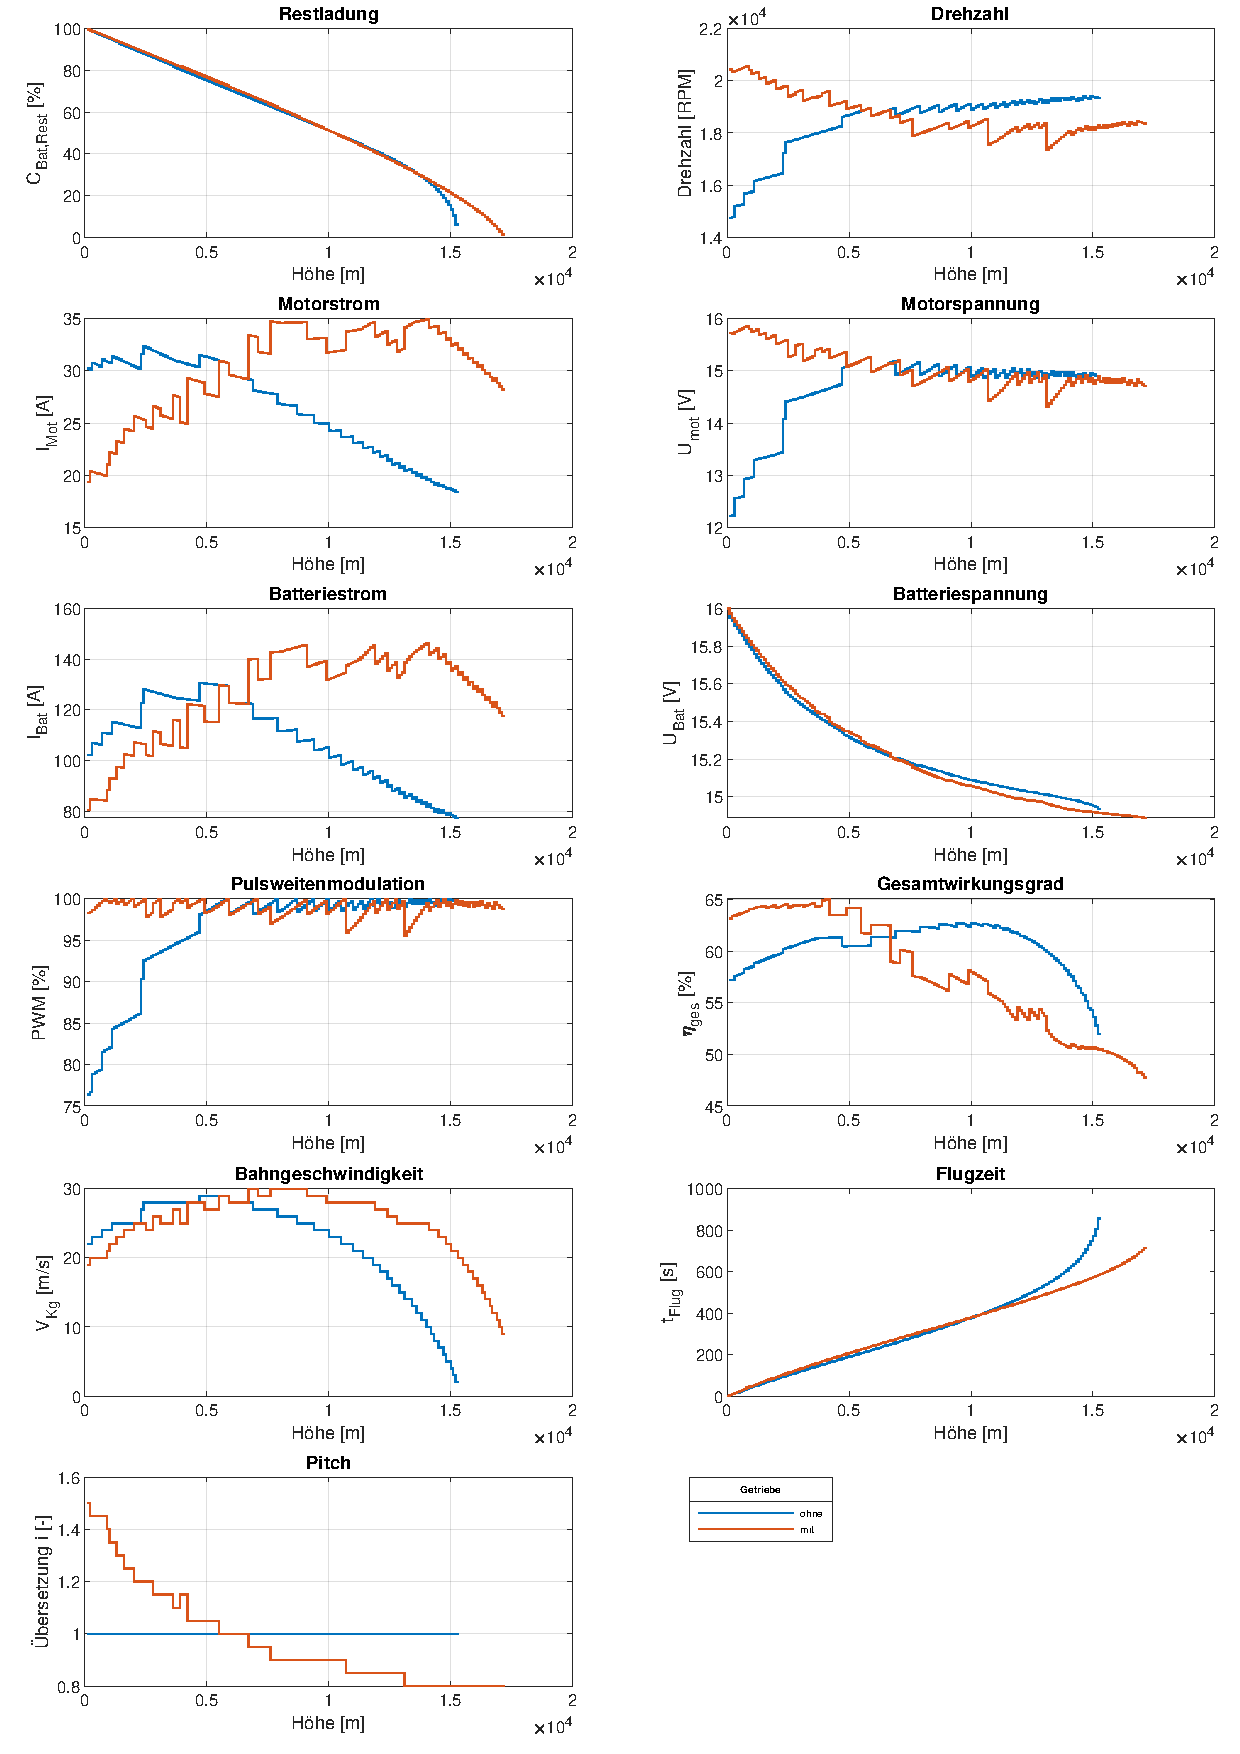
\includegraphics[scale=0.7]{Diagramme/Getriebe.pdf}
	\caption{Einfluss eines idealen (Eigengewicht gleich null und Getriebewirkungsgrad gleich \SI{100}{\%}) Getriebes auf die Flugleistungen der Multicopter-Referenzkonfiguration (Tab. \ref{tab:referenzkonfiguration_mulitcopter})}
	\label{abb:getriebe}
\end{figure}
Der Einsatz eines idealen, stufenlosen Getriebes (\ensuremath{m_{Getriebe} = 0} und \ensuremath{\eta_{Getriebe} = 1}) bietet nur minimale Vorteile (vgl. Abb. \ref{abb:getriebe}). Durch das Getriebe ist die Restladung im Durchschnitt um \SI{2}{\%} größer als ohne. Aus der Reihenfolge des Programms ist die Übersetzung der Drehzahlen und Drehmomente genau umgekehrt. In diesem wird die Drehzahl des Propellers für den Motor angepasst. Mit dieser Blickweise wird die Motordrehzahl zuerst ins Schnelle übersetzt und anschließend ab ca. \SI{15000}{m} Höhe ins Langsame. Auf Grund der Tatsache, dass die Leistung über einem Getriebe konstant bleibt und hier vorerst keine weiteren Verluste berücksichtigt werden, ist der Verlauf des Drehmoments komplementär zu dem Drehzahl, sodass die Beziehung in Gleichung \ref{eq:getriebe_leistung} erhalten bleibt. \\
Die Übersetzung hat keinen Einfluss auf die Propellerdrehzahl. Diese wird durch Interpolation aus dem Propellerkennfeld bestimmt (vgl. Kap. \ref{subsec:propellerzustand}). Die bemerkbaren Unterschiede in Abb. \ref{abb:getriebe} ergeben sich durch die Diskretisierung der Getriebeübersetzung.
Ähnlich kleine Unterschiede weist auch die Bahngeschwindigkeit auf. Dementsprechend klein sind die auch die Unterschiede in der Flugzeit. Das stufenlose Getriebe übersetzt hauptsächlich die Drehzahl des Propellers derart, dass der Motor eine beinahe konstante Spannung erfährt von ca. \SI{17}{V}. Die Motorspannung sinkt dabei leicht mit der Höhe auf \SI{16}{V}. Verantwortlich für die konstante Motorspannung ist die Übersetzung, die beinahe hyperbolisch von anfangs 2 auf 0,9 abnimmt. Der Motorstrom ist durch die Übersetzung des Drehmoments zu Beginn bei \SI{17}{A} und steigt kontinuierlich auf \SI{35}{A}, dem maximalen Motorstrom \ensuremath{I_{max}}. Entsprechend zur Motorspannung bleibt auch die PWM konstant bei ca. \SI{74}{\%}. Dies kennzeichnet einen effizienten Flugzustand, der sich durch einen höheren Gesamtwirkungsgrad \ensuremath{\eta_{ges}} im Gegensatz zur Referenzkonfiguration auszeichnet.

\begin{figure}[H]
\centering
	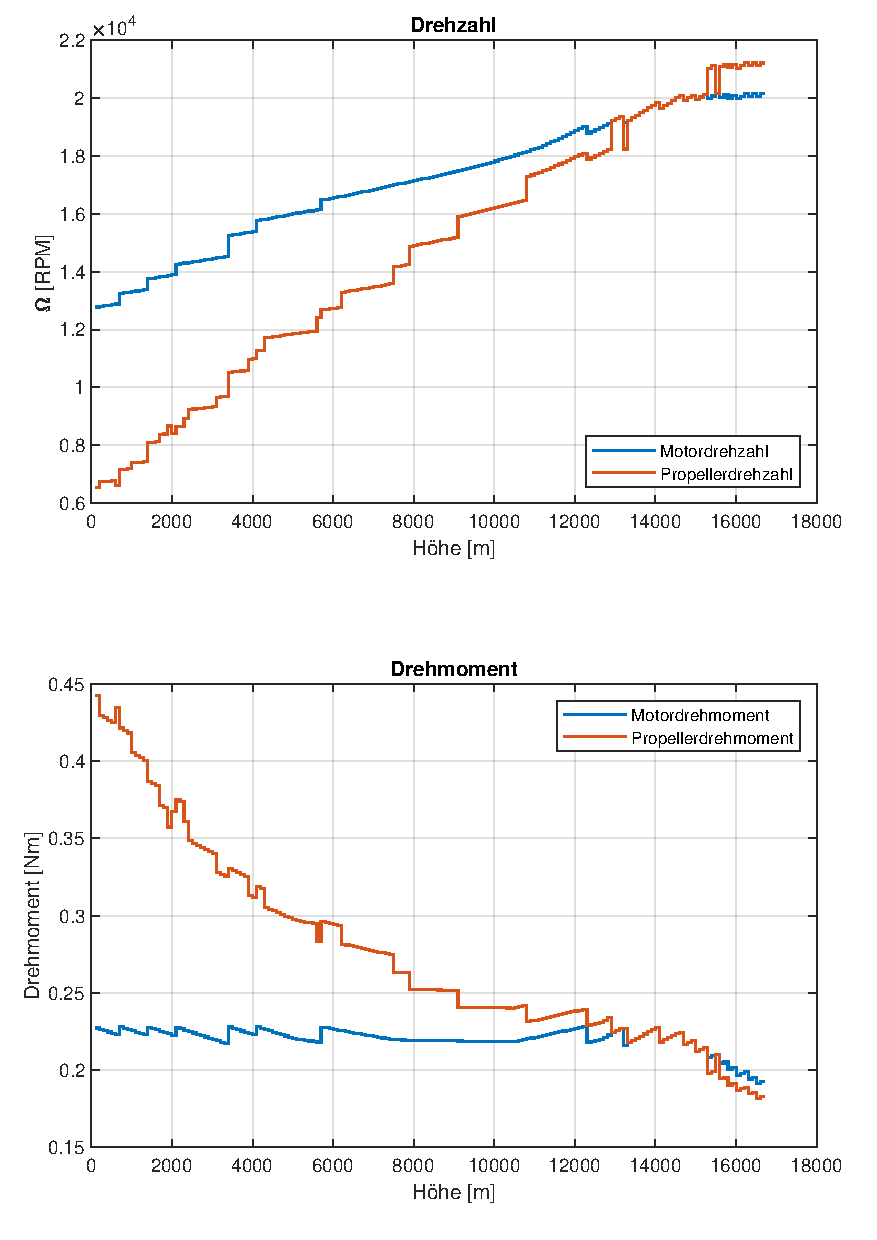
\includegraphics[scale=0.5]{Diagramme/Drehzahl_und_Drehmoment.pdf}
	\caption{Auswirkungen der Übersetzung des Getriebes auf die Drehzahl und das Drehmoment von Motor und Propeller}
	\label{abb:getriebe_dud}
\end{figure}

In der Realität besitzt ein stufenloses Getriebe oder CVT-Getriebe jedoch immer ein Eigengewicht und zeichnet sich durch einen vergleichsweise schlechten Wirkungsgrad aus \cite[S.295-S.297]{Fischer.2016}. %(\SI{0.8}{} zu etwa \SI{0.95}{} bei einem Stufengetriebe)
Die hohen Verluste können auf die hohe erforderliche Reibkraft und Verstellkraft zurückgeführt werden. Unter Berücksichtigung dieser verringert sich der Höhengewinn schrittweise, je größer das Getriebegewicht und dessen Verluste ausfallen. 
Zusätzlich ist anzuzweifeln, dass stufenlos verstellbare Getriebe im Modellbau existieren, die ein sehr geringes Eigengewicht besitzen und sich daher für Flugmodell eignen.
Das Gewicht eines einzelnen Getriebes beläuft sich dabei auf mehr als \SI{750}{g} \cite{cvt}, wobei die Verstellelektronik nicht berücksichtigt wurde. Für einen vierrotorigen Multicopter entspräche das einem Zusatzgewicht von mehr als \SI{3000}{g}. 
Die Vorteile eines CVT-Getriebes werden durch dessen Nachteile deutlich überkompensiert. Ein solches Getriebe bedeutet bei all seiner Kampaktheit und Effizienz letztendlich große Zusatzmasse und einen weiteren, verlustbehaftete Komponenten innerhalb der Antriebskette. Aus all diesen Gründen kann von dem Einsatz eines stufenlosen Getriebes für einen Multicopter abgesehen werden.


\section{Endergebnis}
\label{sec:Endergbnis}
Aus den bisherigen Parameteruntersuchung soll nun eine optimale Konfiguration vorgestellt werden.
Für den Antrieb ist ein Motor mit hohem \ensuremath{K_V}-Wert zu wählen, der zusätzlich wenige interne Verluste hat (vgl. Abschn. \ref{subsec:mot_prop_kombi}). In Bezug auf den gewählten Motor ist der Propeller auszuwählen. Eine Minimierung der aerodynamischen Verluste trägt zu einer Effizienzsteigerung bei (vgl. Kap. \ref{subsec:widerstandseinfluss}). Einen großen Einfluss auf die Flugleistungen hat die Batterie. Kurz zusammengefasst sollte die Batteriemasse einen Anteil von 2/3 der Gesamtmasse einnehmen (vgl. Kap. \ref{sec:massenverteilung}). Dabei ist die Batteriezellenanzahl in Bezug auf den Motor festzulegen (vgl. Kap. \ref{subsec:einfluss_n_bat}).
Die optimale Anzahl der Propeller liegt zwischen vier und acht Propellern (vgl. Kap. \ref{subsubsec:anz_prop}). Es gibt kaum Unterschiede in den Flugleistungen dieser Konfigurationen. Ein Verstellpropeller bringt gewisse Vorteile mit, die die Dienstgipfelhöhe und den anschließenden Sinkflug betreffen, allerdings werden diese durch die zusätzlichen Verluste überkompensiert (vgl. Kap. \ref{sec:verstellprop}). Dies betrifft ebenso den hypothetischen Einsatz eines stufenlos verstellbaren Getriebes (vgl. Kap. \ref{sec:getriebe}). \\
Die optimale Konfiguration ist in Tab. \ref{tab:optimale_konfiguration} konkretisiert. Hierbei sind die Windgeschwindigkeit \ensuremath{u_{Wg}} auf \SI{10}{m/s} gesetzt und die Nutzlast auf \SI{0}{kg}.

\begin{center}
	\captionof{table}{wichtige Parameter der optimalen Multicopter-Konfiguration}
	\begin{tabular}{l l l} \hline
		Parameter & Variablenname & verwendete Größe \\ \hline
		Gesamtmasse \ensuremath{m} & \texttt{m} & \SI{3,078}{kg} \\
		Leermasse des Multicopters \ensuremath{m_{copter}}& \texttt{m\_copter} & \SI{1.028}{kg} \\ 
		Batteriemasse \ensuremath{m_{Bat}} & \texttt{m\_Bat} & \SI{2,052}{kg} \\
		Motormasse \ensuremath{m_{Mot}}& \texttt{m\_Mot} & \SI{106}{g} \\
		Geschwindigkeitskonstante \ensuremath{K_V} & \texttt{K\_V} & \SI{1390}{RPM/V} \\
		maximaler Dauerstrom \ensuremath{I_{max}} & \texttt{I\_max} & \SI{35}{A} \\
		Propeller & \texttt{prop\_name} & 11x4 \\
		Anzahl Propeller \ensuremath{n_{Prop}} & \texttt{n\_prop} & \SI{4}{} \\ 
		Anzahl der Batteriezellen \ensuremath{N_{Bat,cell}} & \texttt{N\_bat\_cell} & 5 \\	 
		Obere Stirnfläche \ensuremath{F_{copter,oben}} & \texttt{F\-copter\_oben} & \SI{0,0209}{m^2} \\
		Oberer Widerstandsbeiwert \ensuremath{c_{W,copter,oben}} & \texttt{c\_W\_copter\_oben} & 0,5 \\ \hline
	\end{tabular}	
	\label{tab:optimale_konfiguration}
\end{center}

Die bestmögliche Konfiguration erreicht bereits eine Dienstgipfelhöhe von  mehr als \SI{18000}{m}. Die Batterie weist auf der Höhe von \SI{15000}{m} noch mehr als \SI{40}{\%} Restladung auf. Mit dieser Restladung ist somit im Anschluss an den Steigflug noch sicherer Sinkflug möglich, sodass das Fluggerät unbeschadet wieder landen kann.

\begin{figure}[H]
\centering
	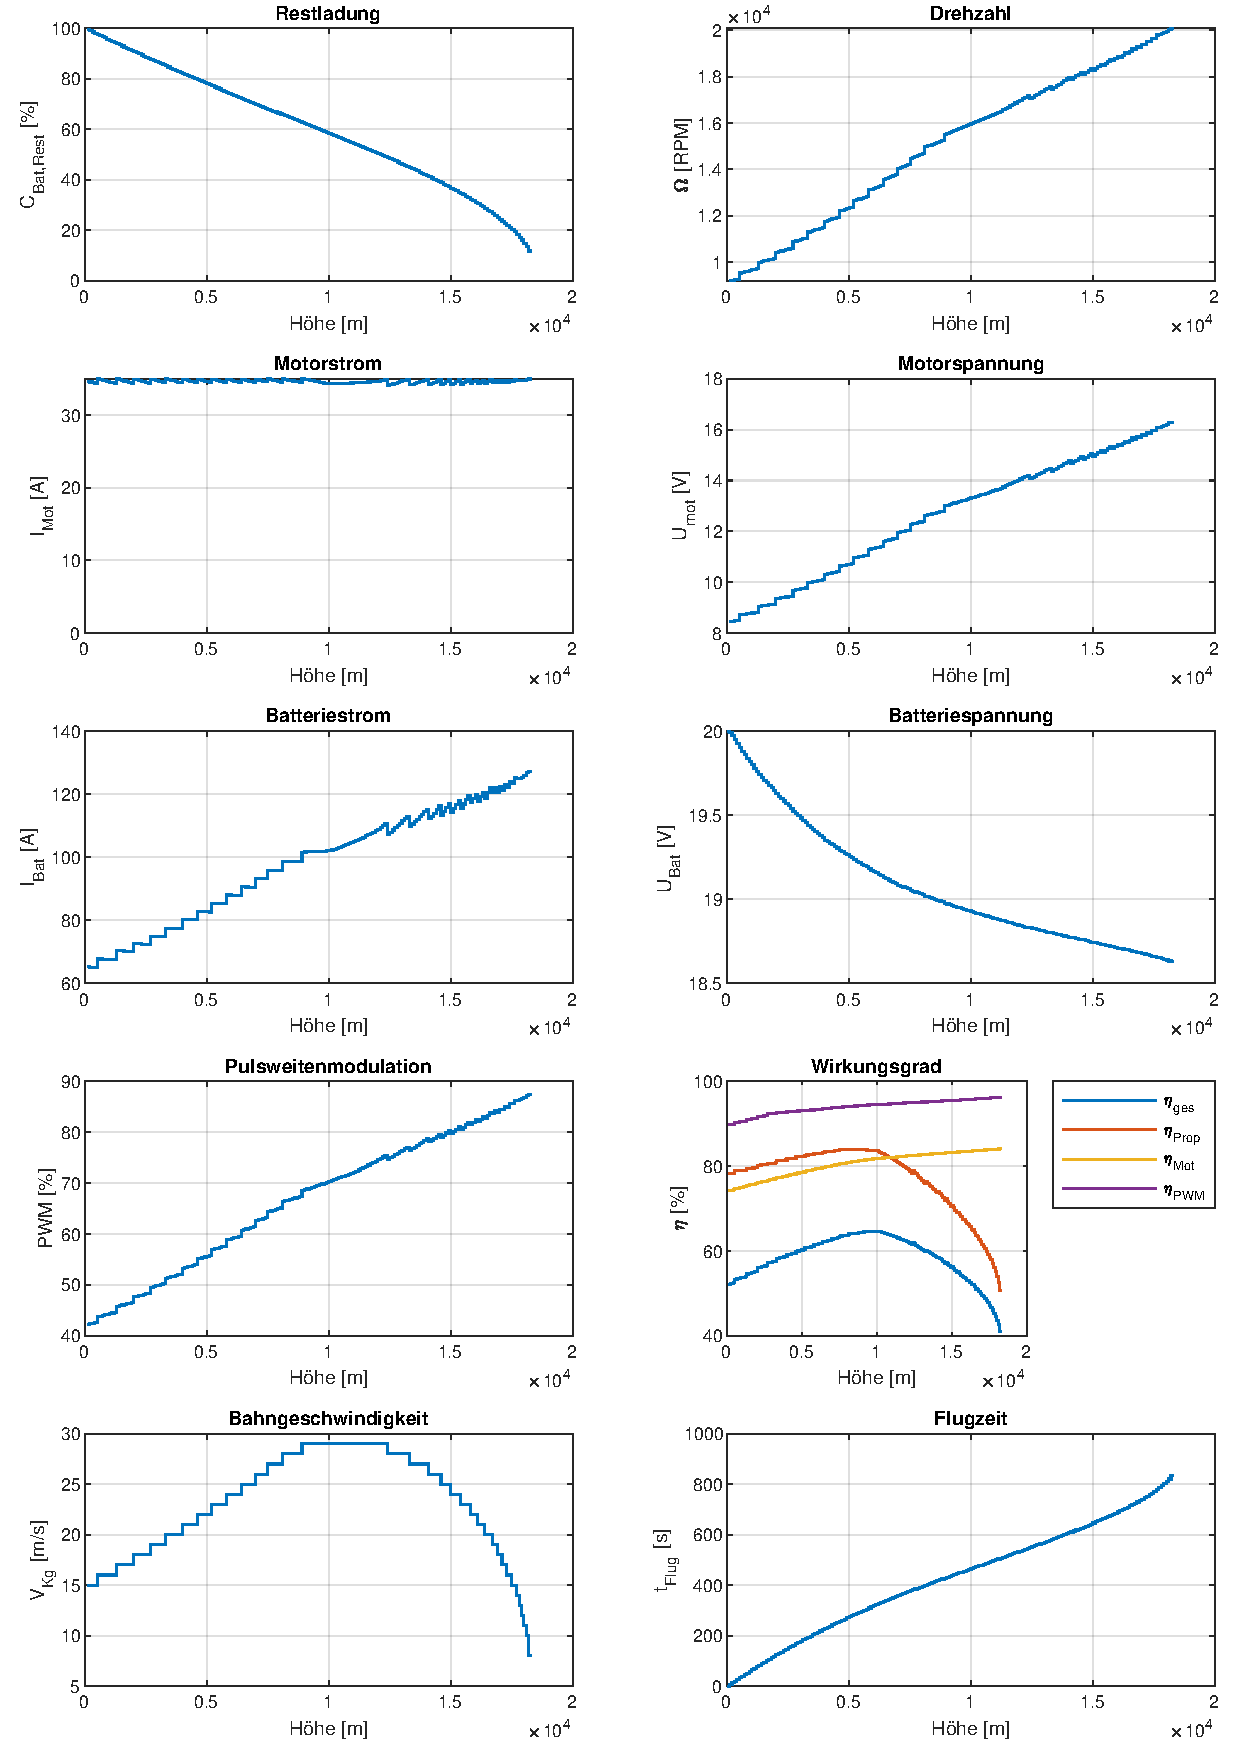
\includegraphics[scale=0.7]{Diagramme/Endergebnis.pdf}
	\caption{Die Flugleistungen der bestmöglichen Konfiguration (Tab. \ref{tab:optimale_konfiguration})}
	\label{abb:optimale_konfig}
\end{figure}


\section{Randbedingungen des AEROMET\_UAV-Projekts}
\label{sec:aeromet_rb}
Schlussendlich soll noch der Einfluss der für dieses Projekt definierten Randbedingungen festgehalten werden. Die für das Projekt vorgeschriebenen Randbedingungen sind in Tab. \ref{tab:randbedingungen} aufgelistet. 
 
\begin{center}
\captionof{table}{wichtige Parameter des Flächenflugzeugs}
\begin{tabular}{l l l} \hline
	Parameter & Variablenname & Wert \\ \hline
	Windgeschwindigkeit \ensuremath{u_{Wg}} & \texttt{u\_Wg} & \SI{100}{km/h}\\
	Nutzlast \ensuremath{m_{Nutz}} & \texttt{m\_Nutz} & \SI{250}{g}  \\ \hline
\end{tabular}	
\label{tab:randbedingungen}
\end{center}

Mit den in Tab. \ref{tab:randbedingungen} definierten Randbedingungen erreicht der Quadrocopter nur noch eine Höhe von \SI{12000}{m} (vgl. Abb. \ref{abb:aeromet_rb}). Die Batteriemasse ist für diesen Flug jedoch auf \SI{50}{\%} des Gesamtgewichts festgesetzt. Mit diesen Ergebnissen ist es für einen Multicopter unwahrscheinlich, dass er unter den AEROMET\_UAV-Randbedingungen eine Höhe von \SI{15000}{m} erreichen kann. Die \SI{10000}{m}-Höhenmarke ist in dem Sinne noch wahrscheinlicher. Wird jedoch ein Minimum von \SI{30}{\%} Restladung am TOC vorgeschrieben, sind selbst \SI{10000}{m} Höhe als kritisch zu bewerten. Unter günstigeren Umgebungsbedingungen sind jedoch wahrscheinlich beide angesetzten Ziele zu erreichen (vgl. Kap. \ref{sec:Endergbnis}).

\begin{figure}[H]
\centering
	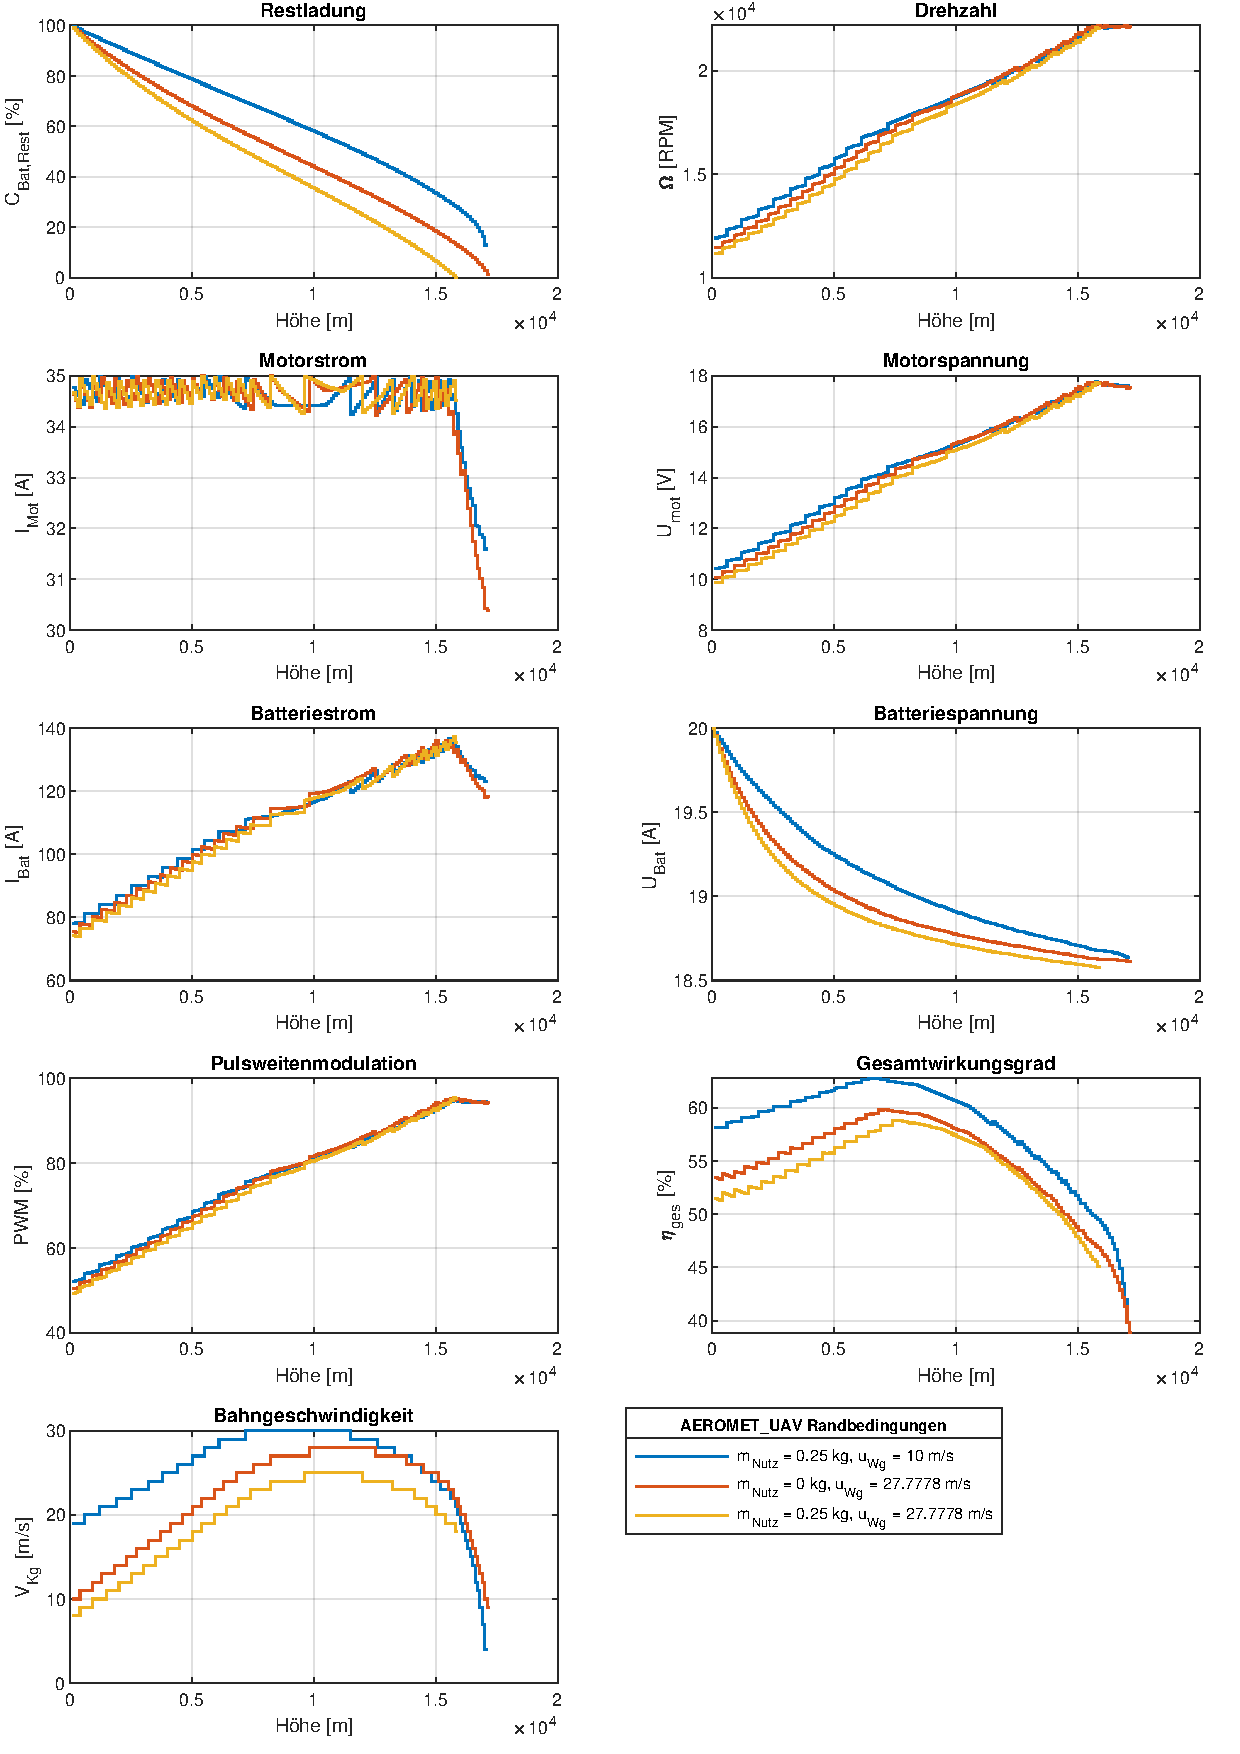
\includegraphics[scale=0.7]{Diagramme/aeromet_randbedingungen.pdf}
	\caption{Einfluss der AEROMET\_UAV-Randbedingungen auf die bestmögliche Konfiguration (Tab. \ref{tab:optimale_konfiguration})}
	\label{abb:aeromet_rb}
\end{figure}